\documentclass[12pt,a4paper,twoside]{book}

% ==========================================
% PAQUETES BÁSICOS
% ==========================================
\usepackage[utf8]{inputenc}
\usepackage[spanish,es-tabla]{babel} % Idioma español
\usepackage{csquotes} % Recomendado por biblatex con babel
\usepackage[T1]{fontenc}
\usepackage{lmodern}
\usepackage{microtype}
\usepackage{indentfirst}
\usepackage{titlesec}
\usepackage{needspace}
\usepackage{pdflscape}

% ==========================================
% MÁRGENES Y FORMATO
% ==========================================
\usepackage[top=3cm, bottom=3cm, left=3.5cm, right=2.5cm]{geometry}
\usepackage{setspace}
\onehalfspacing
\emergencystretch=2em
\raggedbottom
\setlength{\parindent}{1.25em}
\setlength{\parskip}{0pt}
\clubpenalty=10000
\widowpenalty=10000
\displaywidowpenalty=10000

% ==========================================
% GRÁFICOS, TABLAS Y CÓDIGO
% ==========================================
\usepackage{graphicx}
\graphicspath{{figuras/}}
\usepackage{booktabs}
\usepackage{float}
\usepackage{listings}
\usepackage{xcolor}
\usepackage{xurl}
\usepackage{tikz}
\usepackage{multirow}       % Celdas multi-fila en tablas
\usepackage{tabularx}       % Tablas con ancho ajustable
\usepackage{pgfgantt}        % Diagramas de GANTT
\usepackage{pgfplots}        % Gráficos de barras y líneas
\pgfplotsset{compat=1.18}
\usepackage{eurosym}         % Símbolo del euro
\usepackage{amsmath}         % Ecuaciones matemáticas
\usepackage{amssymb}         % Símbolos matemáticos

\usetikzlibrary{arrows.meta,positioning,shapes.geometric,fit,backgrounds}
\definecolor{codegreen}{rgb}{0,0.6,0}
\definecolor{codegray}{rgb}{0.5,0.5,0.5}
\definecolor{codepurple}{rgb}{0.58,0,0.82}
\definecolor{backcolour}{rgb}{0.95,0.95,0.92}

\lstdefinestyle{mystyle}{
    backgroundcolor=\color{backcolour},   
    commentstyle=\color{codegreen},
    keywordstyle=\color{magenta},
    numberstyle=\tiny\color{codegray},
    stringstyle=\color{codepurple},
    basicstyle=\ttfamily\footnotesize,
    breakatwhitespace=false,         
    breaklines=true,                 
    captionpos=b,                    
    keepspaces=true,                 
    numbers=left,                    
    numbersep=5pt,                  
    showspaces=false,                
    showstringspaces=false,
    showtabs=false,                  
    tabsize=2
}
\lstset{style=mystyle}

\titleformat{\section}
  {\normalfont\Large\bfseries}
  {\thesection}
  {0.8em}
  {}
\titleformat{\subsection}
  {\normalfont\large\bfseries}
  {\thesubsection}
  {0.8em}
  {}
\titleformat{\subsubsection}
  {\normalfont\normalsize\bfseries}
  {\thesubsubsection}
  {0.8em}
  {}

\titlespacing*{\section}{0pt}{2.8ex plus 0.8ex minus 0.3ex}{1.2ex}
\titlespacing*{\subsection}{0pt}{2.2ex plus 0.6ex minus 0.2ex}{0.8ex}
\titlespacing*{\subsubsection}{0pt}{1.8ex plus 0.4ex minus 0.2ex}{0.6ex}

\pretocmd{\section}{\needspace{8\baselineskip}}{}{}
\pretocmd{\subsection}{\needspace{6\baselineskip}}{}{}
\pretocmd{\subsubsection}{\needspace{5\baselineskip}}{}{}

\newcommand{\modebadge}[2]{%
    \begingroup
    \setlength{\fboxsep}{4pt}%
    \colorbox{#1!18}{\textcolor{black}{\texttt{#2}}}%
    \endgroup
}

% ==========================================
% BIBLIOGRAFÍA Y ENLACES
% ==========================================
\usepackage[
    backend=biber,
    style=ieee,
    sorting=none,
    url=true,
    doi=true
]{biblatex}
\addbibresource{bibliografia.bib}

\usepackage[colorlinks=true, linkcolor=black, citecolor=blue, urlcolor=blue]{hyperref}

% ==========================================
% DOCUMENTO PRINCIPAL
% ==========================================
\begin{document}

\frontmatter

\begin{titlepage}
    \centering
    \vspace*{1cm}
    
    
\includegraphics[width=0.4\textwidth]{logo_urjc.jpg}\par\vspace{1cm}
    {\scshape\LARGE Universidad Rey Juan Carlos \par}
    \vspace{1.5cm}
    {\scshape\Large Trabajo de Fin de Grado\par}
    \vspace{1.5cm}
    
    {\Huge\bfseries JARVIS RAG:\par}
    {\Large\bfseries Sistema Local de Consulta Documental con Generación Aumentada mediante Recuperación\par}
    
    \vspace{2cm}
    {\Large\itshape Autor:\par}
    {\Large Ángel María Ballesteros Limones\par}
    
    \vfill
    {\large Tutor:\par}
    {\large Jesús María González Barahona\par}
    
    \vfill
    {\large Grado en Ingeniería de Tecnología de Telecomunicaciones\par}
    {\large Curso 2025/2026\par}

\end{titlepage}

\include{dedicatoria}
\chapter*{Agradecimientos}
\addcontentsline{toc}{chapter}{Agradecimientos}

Este proyecto no habría sido posible sin el apoyo y la colaboración de numerosas personas e instituciones que han contribuido, directa o indirectamente, a su realización.

En primer lugar, quiero agradecer a mi tutor de TFG por su orientación académica y su disponibilidad a lo largo de todo el proceso de desarrollo, siendo nuestros horarios tan diferentes. Sus revisiones y conocimiento han sido determinantes para conseguir dar forma a la idea que tenía en mente.

Agradezco también a la empresa Europavia por facilitar el entorno real de despliegue, con una necesidad existente a nivel corporativo que ha servido como banco de pruebas del sistema. La oportunidad de desarrollar un proyecto con impacto práctico inmediato en un contexto profesional ha enriquecido enormemente la experiencia. Sobre todo Nacho y CIVEX por ser siempre de ayuda y facilitar cualquier desarrollo que considerara.

A mis compañeros de carrera, sobre todo a los de Rugby y a aquellos del Erasmus, que me enseñaron el verdadero sentido de la universidad. El camino se hace más llevadero cuando se recorre en buena compañía.

A mi familia, por su paciencia infinita durante los meses más intensos de exámenes. Su apoyo incondicional ha sido el pilar fundamental sobre el que se sustenta todo lo demás.

Por último, quiero reconocer a la comunidad de código abierto, cuyos proyectos --- Ollama, Qdrant, FastAPI, OpenWebUI, Playwright, PaddleOCR, LiteLLM, entre muchos otros --- han hecho posible construir un sistema de esta envergadura sin dependencias comerciales. Este TFG es, en gran medida, un tributo a la filosofía del software libre.

\vspace{1cm}
\begin{flushright}
\textit{Ángel María Ballesteros Limones}\\
\textit{Madrid, 2026}
\end{flushright}
\newpage

\chapter*{Resumen}
\addcontentsline{toc}{chapter}{Resumen}

Este Trabajo de Fin de Grado presenta el diseño, desarrollo y despliegue de un sistema de Generación Aumentada mediante Recuperación (\textit{Retrieval-Augmented Generation}, RAG) de ámbito corporativo, ejecutado íntegramente en infraestructura local (\textit{on-premise}) e integrando herramientas y modelos de código abierto con desarrollo propio.

El sistema permite consultar en lenguaje natural los documentos internos de una organización, páginas web y fuentes legislativas oficiales, respondiendo siempre con las fuentes citadas. Una pila de microservicios contenerizados con Docker integra modelos de lenguaje locales (Ollama), una base de datos vectorial (Qdrant) y un agente encaminador denominado JARVIS que detecta la intención de cada consulta y la delega al modo de operación más adecuado. Entre las fuentes integradas destacan Microsoft SharePoint ---principal entorno de validación práctica---, páginas web extraídas mediante scraping, documentos escaneados tratados con OCR acelerado por GPU y el Boletín Oficial del Estado.

El sistema ha sido desplegado y validado en un entorno real con resultados satisfactorios: tiempos de respuesta inferiores a 3.5 segundos y una reducción muy significativa de las alucinaciones en modo RAG gracias a una estrategia de recuperación documental orientada a la trazabilidad.

\vspace{0.5cm}
\noindent\textbf{Palabras clave:} RAG, LLM, inteligencia artificial, embeddings, base de datos vectorial, microservicios, Docker, Ollama, Qdrant, on-premise, código abierto.

\newpage

\chapter*{Abstract}
\addcontentsline{toc}{chapter}{Abstract}

This Bachelor's Thesis presents the design, development and deployment of a corporate Retrieval-Augmented Generation (RAG) system, executed entirely on local infrastructure (on-premise) and built by integrating open-source tools and models together with original development.

The system allows the internal documents of an organization, web pages and official legislative sources to be queried in natural language, always answering with cited sources. A stack of Docker-containerized microservices integrates locally executed language models (Ollama), a vector database (Qdrant) and a routing agent called JARVIS, which detects the intent of each query and delegates it to the most suitable operating mode. Integrated sources include Microsoft SharePoint ---the main real-world validation environment---, web pages processed through scraping, scanned documents handled with GPU-accelerated OCR, and the Spanish Official State Gazette (BOE).

The system has been deployed and validated in a real environment with satisfactory results: response times under 3.5 seconds and a very significant reduction of hallucinations in RAG mode thanks to a document retrieval strategy focused on traceability.

\vspace{0.5cm}
\noindent\textbf{Keywords:} RAG, LLM, artificial intelligence, embeddings, vector database, microservices, Docker, Ollama, Qdrant, on-premise, open source.

\newpage


\tableofcontents
\listoffigures
\listoftables

\mainmatter

\chapter{Introducción}
\label{cap:intro}

% ============================================================
\section{Motivación}
% ============================================================

En los entornos corporativos actuales, el volumen de información disponible crece de forma constante, pero no crece de forma ordenada. La documentación relevante suele estar repartida entre repositorios como Microsoft SharePoint, PDFs internos, muchos de ellos escaneados, wikis, portales de proveedores, procedimientos técnicos y fuentes públicas como el Boletín Oficial del Estado (BOE). En la práctica, el problema habitual no es la falta de información, sino la dispersión, la heterogeneidad de formatos y la dificultad para recuperar contenido útil cuando se necesita.

Los métodos tradicionales de búsqueda por palabras clave fallan en situaciones muy comunes: cuando el usuario no conoce el término exacto, cuando la información está contenida en documentos largos, cuando existen sinónimos o acrónimos internos, o cuando el contenido está en PDFs escaneados y requiere OCR. Como consecuencia, tareas rutinarias como confirmar un procedimiento, localizar un requisito normativo o recuperar una especificación se convierten en procesos lentos y propensos a errores.

En paralelo, la popularización de los grandes modelos de lenguaje (LLMs, \textit{Large Language Models}) ha permitido interactuar con sistemas de información mediante lenguaje natural. Sin embargo, en un contexto corporativo, una respuesta fluida pero incorrecta tiene un coste elevado: puede inducir decisiones erróneas y generar confianza injustificada. El problema se agrava cuando el modelo no dispone de acceso al conocimiento interno, cuando la documentación cambia con frecuencia o cuando la consulta requiere precisión y respaldo documental.

Por este motivo, resulta especialmente relevante el enfoque de Generación Aumentada mediante Recuperación (RAG, \textit{Retrieval-Augmented Generation}), que combina la generación de lenguaje con la recuperación de información desde una base documental. En lugar de responder de memoria, el sistema fundamenta la respuesta en documentos recuperados, mejorando la utilidad, la trazabilidad y reduciendo la probabilidad de respuestas no justificadas \cite{lewis2020rag}.

Este Trabajo de Fin de Grado no parte de entrenar un modelo desde cero. Sería un objetivo desproporcionado para el alcance del proyecto y, además, no resolvería por sí mismo el problema principal, que no es crear otro LLM generalista, sino poner modelos ya existentes a trabajar de forma útil, segura y controlada sobre información corporativa cambiante. Por ello, el trabajo se centra en seleccionar, integrar, adaptar y orquestar tecnologías existentes de código abierto y pesos abiertos: modelos de lenguaje ejecutados localmente, embeddings, una base de datos vectorial, un backend propio en Python, mecanismos de ingesta documental y una interfaz conversacional empresarial.

Con esta motivación, el proyecto aborda el diseño, desarrollo e integración de un sistema RAG corporativo desplegado en infraestructura controlada (\textit{on-premise}), capaz de ingerir documentos desde fuentes heterogéneas y ofrecer a los usuarios una interfaz conversacional orientada a consultas técnicas, con recuperación semántica y soporte documental.

% ============================================================
\subsection{Problemática del Shadow AI en entornos corporativos}
\label{subsec:shadow_ai}
% ============================================================

La adopción de asistentes de IA comerciales en el ámbito laboral ha impulsado un fenómeno cada vez más habitual: el uso no autorizado de herramientas externas por parte de empleados sin supervisión del departamento de TI ni revisión legal o de cumplimiento. Este patrón se conoce como \textit{Shadow AI} y puede considerarse una extensión del \textit{Shadow IT}, con un riesgo añadido: la exposición de datos puede producirse en el mismo momento en que un usuario copia y pega información interna en un servicio externo \cite{microsoft2024worktrend}.

La magnitud del fenómeno es considerable. Según el informe \textit{Work Trend Index} de Microsoft y LinkedIn (2024), el 75\% de los trabajadores del conocimiento utiliza herramientas de IA en su trabajo, y el 78\% de ellos emplea herramientas propias no autorizadas por la organización \cite{microsoft2024worktrend}. En un análisis de Cyberhaven sobre 1,6 millones de trabajadores, se detectó que el 8,6\% de los empleados introducía datos corporativos en ChatGPT, y que el 11\% de esos datos estaba clasificado como confidencial \cite{cyberhaven2024shadow}. Además, entre marzo de 2023 y marzo de 2024, la cantidad de datos corporativos introducidos en herramientas de IA se multiplicó por 4,85, y la proporción de datos sensibles casi se triplicó, pasando del 10,7\% al 27,4\% \cite{kalisa2024shadow}.

Los riesgos principales asociados a este fenómeno son:

\begin{itemize}
    \item \textit{Exposición de información sensible}: al introducir documentos, fragmentos de procedimientos, incidencias, datos operativos o contenido contractual en herramientas externas, la información puede salir del perímetro de seguridad corporativo. Un estudio de Komprise (2025) reveló que el 44\% de las organizaciones ha experimentado fugas de datos sensibles hacia herramientas de IA \cite{komprise2025survey}.
    \item \textit{Riesgo regulatorio y de cumplimiento}: en sectores regulados o con datos personales o sensibles, el tratamiento de la información exige garantías sobre finalidad, acceso, ubicación y medidas de seguridad. El uso informal de herramientas externas introduce incertidumbre y eleva el riesgo de incumplimiento normativo.
    \item \textit{Calidad y consistencia}: los modelos generalistas pueden producir respuestas plausibles incluso cuando carecen de base documental. En ámbitos técnicos o normativos, esto se traduce en errores silenciosos con apariencia de certeza.
    \item \textit{Ausencia de gobernanza}: sin control centralizado, la organización no sabe qué herramientas se usan, con qué datos, con qué finalidad ni con qué impacto.
\end{itemize}

Este proyecto aborda directamente esta problemática mediante una alternativa interna: un sistema conversacional desplegado en la infraestructura de la organización, donde los documentos no se envían a servicios externos y donde las respuestas se apoyan en recuperación documental, reduciendo respuestas no fundamentadas y permitiendo trazabilidad hacia fuentes internas.

% ============================================================
\section{Solución propuesta y enfoque del trabajo}
\label{sec:solucion}
% ============================================================

La solución propuesta consiste en construir un asistente corporativo que actúe como punto único de acceso a la información de la organización. La idea no es sustituir todos los sistemas documentales existentes, sino superponer una capa de consulta en lenguaje natural que permita a cualquier usuario localizar y comprender información dispersa sin necesidad de conocer de antemano dónde está almacenada ni en qué formato se encuentra.

Para resolver los problemas descritos en la sección anterior, el sistema combina varios bloques:

\begin{itemize}
    \item \textit{Modelos ya existentes ejecutados en local}: se reutilizan LLMs y modelos de embeddings disponibles públicamente, desplegados dentro de la infraestructura propia.
    \item \textit{Un backend propio en Python}: se desarrolla la lógica que conecta los modelos con las fuentes documentales, aplica reglas de acceso y construye respuestas trazables.
    \item \textit{Un pipeline RAG}: antes de responder, el sistema recupera fragmentos relevantes de la documentación para que la generación se apoye en evidencia.
    \item \textit{Conectores e integraciones}: se incorporan mecanismos para trabajar con SharePoint, documentos escaneados, páginas web y normativa del BOE.
    \item \textit{Una interfaz conversacional reutilizable}: en lugar de crear una interfaz desde cero, se aprovecha OpenWebUI y se amplía mediante un pipeline propio.
\end{itemize}

Este enfoque tiene dos ventajas. La primera es práctica: permite construir un sistema funcional en el contexto de un TFG sin depender del entrenamiento masivo de modelos. La segunda es metodológica: separa claramente qué aporta la tecnología base y qué aporta el trabajo realizado en el proyecto. En este caso, la contribución no está en crear un nuevo modelo fundacional, sino en diseñar una arquitectura útil, explicar por qué cada pieza es necesaria y desarrollar la lógica que convierte herramientas sueltas en un sistema corporativo coherente.

% ============================================================
\section{Código del proyecto}
\label{sec:codigo-proyecto}
% ============================================================

Tanto el código fuente como la documentación técnica del proyecto están publicados en GitHub\footnote{\url{https://github.com/acidxlemons/TFG-JARVIS}}. Este repositorio incluye la definición de la arquitectura Docker, los servicios implementados en Python, la configuración de los modelos locales y los materiales necesarios para reproducir el despliegue. Se menciona aquí de forma explícita porque una parte importante del valor del trabajo reside precisamente en la combinación de componentes reutilizados con código propio integrador.

% ============================================================
\section{Objetivos del proyecto}
\label{sec:objetivos}
% ============================================================

El objetivo principal de este trabajo es desarrollar un asistente conversacional corporativo sustentado en una arquitectura RAG \textit{on-premise}, capaz de consultar documentación cambiante almacenada en la nube o en otras fuentes heterogéneas sin sacar los datos del entorno controlado de la organización. Aunque la idea general es poder trabajar con repositorios documentales de distinto tipo, la implementación y las pruebas de este TFG se han realizado principalmente sobre SharePoint como caso real de integración.

La motivación operativa es clara: si los problemas detectados son dispersión documental, formatos heterogéneos, riesgo de \textit{Shadow AI} y falta de trazabilidad, la respuesta técnica debe ser un sistema que recupere información de forma centralizada, la explique con lenguaje natural y deje claro en qué documentos se apoya.

Para alcanzar este objetivo general, se han definido los siguientes objetivos específicos:

\begin{enumerate}
    \item \textit{Diseñar una arquitectura modular reutilizando bloques ya disponibles y añadiendo desarrollo propio donde aporta valor}: combinar modelos de lenguaje locales, embeddings, una base de datos vectorial y una interfaz conversacional, añadiendo un backend en Python que orqueste todo el sistema.

    \item \textit{Permitir ingesta multicanal y actualización de conocimiento}: incorporar carga y actualización documental desde fuentes heterogéneas, con especial foco en SharePoint, incluyendo OCR para documentos escaneados y extracción web cuando sea necesario.

    \item \textit{Ofrecer respuestas fundamentadas y trazables}: implementar un flujo RAG que priorice la recuperación documental frente a la generación libre y muestre al usuario sobre qué fuentes se construye cada respuesta.

    \item \textit{Añadir capacidades complementarias sin entrenar modelos desde cero}: integrar búsqueda web controlada, scraping, análisis de imágenes y consulta normativa del BOE reutilizando herramientas ya disponibles y conectándolas mediante lógica propia.

    \item \textit{Explorar MCP como línea de integración futura}: desarrollar un servidor compatible con el enfoque de Model Context Protocol (MCP) \cite{anthropic2024mcp} para el caso del BOE, dejando preparada una vía de evolución aunque la interfaz web del proyecto siga usando integración por API en la implementación actual.

    \item \textit{Desplegar el sistema de forma reproducible y observable}: contenerizar el ecosistema con Docker y habilitar métricas y paneles de monitorización que permitan operar y analizar el sistema.
\end{enumerate}

% ============================================================
\section{Alcance y limitaciones}
% ============================================================

\subsection{Alcance}

El proyecto cubre el ciclo completo de construcción de un sistema RAG empresarial, desde el diseño de la arquitectura hasta su despliegue reproducible. El alcance real del trabajo se resume en los siguientes puntos:

\begin{itemize}
    \item Selección y despliegue de modelos existentes de lenguaje, visión y embeddings; no se entrena un modelo fundacional desde cero.
    \item Diseño e implementación de una arquitectura basada en microservicios contenerizados.
    \item Desarrollo de un backend propio en Python para orquestación, recuperación documental, control de acceso y conexión con herramientas externas.
    \item Integración de un pipeline de ingesta documental con soporte para PDFs, HTML, imágenes y documentación alojada en SharePoint.
    \item Construcción de un motor de búsqueda semántica basado en embeddings y almacenamiento vectorial.
    \item Reutilización de OpenWebUI como interfaz conversacional e integración de su autenticación con el proveedor corporativo de identidad mediante OIDC/Azure AD.
    \item Extensión de OpenWebUI mediante un pipeline propio que añade encaminamiento, memoria de sesión y control de acceso documental.
    \item Integración funcional con fuentes externas como SharePoint, BOE e Internet.
    \item Desarrollo de un servidor MCP para normativa del BOE como prueba de concepto técnica orientada a futuras integraciones.
    \item Incorporación de un stack de monitorización y observabilidad para analizar uso y rendimiento.
\end{itemize}

En otras palabras, el alcance combina dos tipos de trabajo. Por un lado, se reutilizan componentes ya maduros, como OpenWebUI, Ollama, Qdrant o PaddleOCR. Por otro, se desarrollan específicamente para el TFG las piezas que faltaban para convertirlos en un sistema coherente: el backend RAG, el pipeline JARVIS, el indexador, la integración BOE y la configuración operativa del despliegue.

En relación con MCP, conviene precisar el alcance para evitar ambigüedades: en este TFG no se desarrolla un cliente MCP completo dentro de la interfaz web, sino un servidor MCP propio validado en entorno compatible. La funcionalidad visible por el usuario final se presta actualmente mediante llamadas a API, mientras que MCP queda como capacidad implementada y preparada para evolucionar.

\subsection{Limitaciones}

Se identifican las siguientes limitaciones reconocidas:

\begin{itemize}
    \item \textit{Requisitos hardware}: el sistema requiere una GPU NVIDIA con suficiente VRAM para mantener un rendimiento aceptable en tareas de OCR e inferencia local.

    \item \textit{Predominio de SharePoint en la validación}: aunque la arquitectura está pensada para documentos cambiantes en la nube y de distinta naturaleza, la validación experimental se ha centrado sobre todo en SharePoint, que es la integración más desarrollada del proyecto.

    \item \textit{BOE con doble nivel de integración}: el sistema permite consultas normativas desde la interfaz mediante API, pero la integración MCP nativa en la web no se incorpora todavía por limitaciones del cliente utilizado.

    \item \textit{MCP validado fuera de la interfaz principal}: el servidor MCP desarrollado funciona en entorno de terminal con clientes compatibles, pero su adopción dentro de la interfaz web queda como trabajo futuro.

    \item \textit{Sesgo en el ajuste fino}: el \textit{fine-tuning} LoRA se realiza con datos sintéticos generados a partir del propio sistema base, lo que puede introducir sesgos y limitar la generalización.

    \item \textit{Evaluación acotada}: la evaluación se realiza principalmente de forma funcional y cualitativa; benchmarks académicos más formales quedan fuera del alcance temporal del proyecto.

    \item \textit{Obsolescencia rápida del contexto tecnológico}: el ecosistema de modelos, herramientas y estándares evoluciona a gran velocidad, de modo que algunas decisiones tecnológicas razonables durante el desarrollo pueden quedar superadas en pocos meses.
\end{itemize}

% ============================================================
\section{Contribuciones principales}
% ============================================================

Las contribuciones técnicas concretas de este trabajo son:

\begin{enumerate}
    \item Una arquitectura reproducible basada en microservicios, definida declarativamente en Docker Compose, con servicios orientados a ingesta, almacenamiento, recuperación, generación y monitorización.

    \item Un agente encaminador, JARVIS, capaz de seleccionar distintos modos de operación en función de la intención detectada y de guiar cada consulta hacia el subsistema adecuado.

    \item Un pipeline de ingesta multicanal que unifica SharePoint, scraping web, OCR y carga manual en una única base de conocimiento vectorial.

    \item Una integración funcional con el BOE dentro del sistema, permitiendo búsquedas y consultas normativas desde la experiencia conversacional.

    \item El desarrollo y validación de un servidor MCP para consulta normativa del BOE, operativo fuera de la interfaz principal y planteado como base de evolución futura.

    \item Un flujo de adaptación de modelos base mediante LoRA orientado al dominio del proyecto, evaluado como complemento y no como núcleo de la solución.

    \item La publicación del sistema como proyecto de código abierto en GitHub\footnote{\url{https://github.com/acidxlemons/TFG-JARVIS}}, con documentación para despliegue reproducible.
\end{enumerate}

% ============================================================
\section{Estructura de la memoria}
% ============================================================

El resto de este documento se estructura de la siguiente manera:

En el \textbf{Capítulo~\ref{cap:estado}} se presentan los fundamentos que permiten entender la solución propuesta: qué son los LLMs, por qué un LLM por sí solo no basta en este problema y qué papel desempeñan RAG, los embeddings, las bases vectoriales, la cuantización, LoRA y MCP.

El \textbf{Capítulo~\ref{cap:tecnologias}} aterriza las tecnologías concretas utilizadas en el proyecto, explicando para qué sirve cada una, por qué se ha elegido y cuál es su papel dentro del sistema completo.

El \textbf{Capítulo~\ref{cap:sistemas}} analiza sistemas existentes similares al desarrollado, tanto comerciales como de código abierto, para situar la propuesta dentro del ecosistema actual.

El \textbf{Capítulo~\ref{cap:funcional}} ofrece una descripción funcional completa del sistema desde la perspectiva del usuario: interfaz conversacional, modos de operación, escenarios de uso y panel de administración.

El \textbf{Capítulo~\ref{cap:implementacion}} constituye el núcleo técnico del proyecto. Describe la arquitectura, la separación entre desarrollo propio y herramientas externas, el mecanismo Pipeline de OpenWebUI, el agente JARVIS, el motor RAG y las integraciones principales.

El \textbf{Capítulo~\ref{cap:metodologia}} describe la metodología seguida, las iteraciones de desarrollo, el entorno hardware, el stack tecnológico completo, la estimación de presupuesto y la estrategia de documentación.

El \textbf{Capítulo~\ref{cap:resultados}} presenta los resultados obtenidos: métricas de rendimiento, evaluación funcional y análisis del comportamiento del sistema.

Por último, el \textbf{Capítulo~\ref{cap:conclusiones}} recoge las conclusiones, el grado de consecución de los objetivos y las líneas futuras de trabajo.

\chapter{Fundamentos de la solución propuesta}
\label{cap:estado}

Este capítulo no pretende enumerar todas las tecnologías del sector, sino introducir únicamente los conceptos necesarios para entender la solución desarrollada en este TFG. La idea es guiar al lector desde el problema hasta la arquitectura elegida: primero se explica qué puede aportar un LLM y por qué no basta por sí solo; después se presenta RAG como mecanismo para responder con apoyo documental; y finalmente se describen los componentes que permiten ejecutar todo ello de forma local, controlada y útil en un contexto corporativo.

% ============================================================
\section{Grandes Modelos de Lenguaje (LLMs)}
% ============================================================

Los grandes modelos de lenguaje (LLMs) son modelos neuronales entrenados para predecir el siguiente \textit{token} en una secuencia. El salto de rendimiento moderno llega con la arquitectura \textit{Transformer} \cite{vaswani2017attention}, donde el mecanismo de atención permite capturar relaciones de contexto con mucha más eficacia que arquitecturas previas.

Desde el punto de vista del usuario, un LLM permite dialogar en lenguaje natural, resumir contenido, reformular instrucciones o generar texto coherente. Sin embargo, conviene aclarar un punto importante para este trabajo: un LLM no es una base de datos ni un buscador documental. Si se le pregunta por información corporativa que no forma parte de su entrenamiento o que ha cambiado recientemente, tenderá a responder con estimaciones plausibles, no necesariamente con hechos verificables.

\subsection{Propietarios vs. pesos abiertos}

En la práctica, existen dos formas habituales de utilizar LLMs:

\begin{itemize}
    \item \textit{Modelos propietarios vía API}: ofrecen un producto muy maduro y alto rendimiento, pero implican dependencia de un proveedor externo y procesamiento fuera del perímetro corporativo.
    \item \textit{Modelos de pesos abiertos (\textit{open-weights})}: permiten ejecución local u \textit{on-premise}, lo que habilita mayor control sobre datos, configuración y despliegue.
\end{itemize}

En este proyecto se prioriza el segundo enfoque porque el requisito principal es operar en local. También conviene diferenciar entre \textit{pesos abiertos} y \textit{código abierto}: que un modelo pueda descargarse y ejecutarse localmente no implica necesariamente una licencia plenamente abierta \cite{meta2024llama31hf,google2024gemmaterms,qwen2024qwen25license}.

El sistema desarrollado reutiliza modelos ya existentes, principalmente de la familia Qwen 2.5 y, en fases previas del proyecto, también Llama 3.1, por ser viables en despliegue local y contar con un ecosistema maduro \cite{meta2024llama31,qwen2024qwen25blog}. Esta decisión refuerza la idea central del proyecto: el valor no está en crear un nuevo modelo fundacional, sino en integrarlo correctamente con el conocimiento de la organización.

% ============================================================
\section{Por qué un LLM por sí solo no resuelve este problema}
% ============================================================

El problema abordado en este TFG no consiste en mantener una conversación general, sino en responder sobre documentación interna, normativa y contenidos que cambian con el tiempo. Un LLM aislado presenta varias limitaciones en este escenario:

\begin{itemize}
    \item No conoce por defecto los documentos privados de la organización.
    \item No accede en tiempo real a repositorios documentales salvo que se le conecte explícitamente a ellos.
    \item Puede mezclar conocimiento general con suposiciones plausibles.
    \item No ofrece trazabilidad automática hacia los documentos utilizados.
\end{itemize}

Por ello, aunque los LLMs son la pieza que permite la interacción en lenguaje natural, no constituyen por sí mismos la solución completa. Hace falta una arquitectura adicional que recupere información, filtre fuentes, construya contexto y limite la generación a aquello que realmente se ha encontrado.

% ============================================================
\section{Generación Aumentada mediante Recuperación (RAG)}
% ============================================================

La arquitectura que responde a ese problema es RAG (\textit{Retrieval-Augmented Generation}) \cite{lewis2020rag}. Su idea básica es sencilla: antes de generar una respuesta, el sistema busca fragmentos relevantes de documentos y se los proporciona al modelo como contexto. De esta forma, el LLM deja de apoyarse solo en su memoria estadística y pasa a responder utilizando evidencia concreta.

Un pipeline RAG típico tiene dos fases:

\begin{enumerate}
    \item \textit{Recuperación}: la pregunta del usuario se transforma en una representación numérica y se buscan fragmentos relevantes en una base documental indexada.
    \item \textit{Generación}: el LLM recibe la pregunta junto con ese contexto recuperado y redacta una respuesta basada en él.
\end{enumerate}

Para un lector no técnico, puede entenderse como una combinación entre un buscador y un asistente conversacional. El buscador encuentra la información; el asistente la explica. Esa combinación es la razón por la que RAG encaja mejor en este proyecto que un chatbot convencional.

\subsection{Mejoras prácticas: búsqueda híbrida y memoria acotada}

En un sistema real, RAG no suele quedarse en una búsqueda semántica simple:

\begin{itemize}
    \item \textit{Búsqueda híbrida}: combina una recuperación basada en significado, obtenida al comparar embeddings, con otra basada en coincidencias exactas de palabras, habitualmente implementada con métodos como BM25. Esto evita perder siglas, identificadores, nombres de procedimientos o artículos legales \cite{robertson2009bm25,weaviateHybridDocs,qdrantHybridTutorial}.
    \item \textit{Reordenación y filtrado}: se seleccionan los fragmentos más útiles antes de enviarlos al modelo.
    \item \textit{Memoria conversacional acotada}: se conserva parte del historial cuando aporta contexto, pero evitando que el \textit{prompt} crezca sin control.
\end{itemize}

La solución de este TFG utiliza precisamente esa variante práctica de RAG, porque es la que mejor se adapta a consultas corporativas reales.

% ============================================================
\section{Modelos de Embeddings}
% ============================================================

Los embeddings convierten texto en vectores numéricos donde la cercanía entre vectores representa similitud semántica. De forma intuitiva, puede pensarse que cada texto se transforma en una huella numérica compacta: si dos huellas quedan cerca en ese espacio, sus significados tienden a ser parecidos. Son el mecanismo que permite pasar de una pregunta escrita por una persona a una búsqueda de contenido relacionada por significado y no solo por palabras exactas.

Una medida habitual de similitud es la similitud del coseno:

\begin{equation}
\text{sim}(\mathbf{a}, \mathbf{b}) = \frac{\mathbf{a} \cdot \mathbf{b}}{||\mathbf{a}|| \cdot ||\mathbf{b}||}
\end{equation}

En este proyecto se emplean modelos de SentenceTransformers \cite{reimers2019sentence,sbertDocs}, ya existentes y desplegables en local, porque permiten generar embeddings sin depender de servicios externos. Esta decisión es importante por dos razones: preserva la privacidad y desacopla la búsqueda semántica del proveedor del LLM generativo.

También se explora la adaptación del modelo de embeddings al dominio del proyecto. Esto es relevante porque, en un entorno corporativo, términos internos, acrónimos y nomenclatura especializada pueden no estar bien representados por un modelo genérico.

% ============================================================
\section{Bases de datos vectoriales}
% ============================================================

Una vez calculados los embeddings, hace falta un sistema capaz de almacenarlos y consultarlos con rapidez. Ese papel lo cumplen las bases de datos vectoriales. En lugar de buscar solo texto, permiten buscar vectores parecidos al vector de la consulta.

En colecciones grandes se usan índices aproximados para acelerar la búsqueda. Uno de los enfoques más extendidos es HNSW \cite{malkov2016hnsw}, un grafo navegable jerárquico diseñado para encontrar vecinos cercanos de forma eficiente.

\begin{table}[H]
\centering
\caption{Comparativa de bases de datos vectoriales evaluadas para el proyecto.}
\label{tab:vectordb-comparativa}
\begin{tabular}{lcccc}
\toprule
\textbf{Base de datos} & \textbf{Licencia} & \textbf{On-Premise} & \textbf{Filtrado} & \textbf{Híbrida} \\
\midrule
Qdrant   & Apache 2.0 & Sí & Sí & Sí \\
Weaviate & BSD-3 & Sí & Sí & Sí \\
Milvus   & Apache 2.0 & Sí & Sí & Sí \\
Chroma   & Apache 2.0 & Sí & Limitado & Limitado \\
Pinecone & Propietaria & No (SaaS) & Sí & Parcial \\
\bottomrule
\end{tabular}
\end{table}

Se selecciona Qdrant por ser \textit{on-premise}, por su filtrado por metadatos y por su buen soporte para búsqueda híbrida \cite{qdrantHybridTutorial,qdrantSparseVectors}. Para este TFG no es solo una decisión de rendimiento, sino también de control: permite separar colecciones, añadir metadatos y aplicar restricciones de acceso documentales.

% ============================================================
\section{Cuantización y ejecución local}
\label{sec:cuantizacion}
% ============================================================

Ejecutar LLMs localmente exige gestionar bien los recursos de hardware, especialmente la VRAM de la GPU. La cuantización reduce la precisión numérica de los pesos para disminuir consumo de memoria y hacer viable la inferencia en hardware más modesto.

En el ecosistema local, el formato GGUF se utiliza ampliamente para empaquetar modelos cuantizados junto con sus metadatos \cite{ggmlGgufSpec,hfGgufDocs}. Herramientas como Ollama permiten servir estos modelos por API y simplifican mucho el despliegue \cite{ollamaImportGguf}.

Este concepto es importante para entender una de las decisiones prácticas del proyecto: no basta con elegir un buen modelo, también hay que elegir una variante que realmente pueda ejecutarse en el hardware disponible sin bloquear el resto del sistema.

% ============================================================
\section{Ajuste fino eficiente con LoRA}
\label{sec:lora}
% ============================================================

El ajuste fino (\textit{fine-tuning}) adapta un modelo generalista a un dominio concreto. Sin embargo, reentrenar por completo un LLM moderno está fuera del alcance normal de un TFG y tampoco era el objetivo principal de este trabajo.

La técnica LoRA (\textit{Low-Rank Adaptation}) reduce drásticamente ese coste reentrenando solo una pequeña parte de la red neuronal del modelo, en lugar de modificar todos sus pesos \cite{hu2021lora}. Concretamente, inserta capas adicionales de tamaño muy reducido —matrices de bajo rango— en las capas de atención del transformador y reentrena únicamente esas capas añadidas, dejando los pesos originales congelados. En la práctica, puede entenderse como ampliar la red neuronal con nuevas conexiones especializadas sin tener que reentrenar toda la arquitectura de partida.

Formalmente, el cambio en el peso de una capa se expresa como:

\begin{equation}
W' = W + \Delta W = W + BA
\end{equation}

donde $A$ y $B$ son matrices de rango reducido con $r \ll \min(d,k)$, lo que hace que el número de parámetros entrenables pase de millones a miles.

En este proyecto, LoRA se estudia como una vía de adaptación incremental sobre modelos ya existentes, no como el eje principal de la solución. La experiencia obtenida muestra que, para consultas RAG puras, suele tener más impacto un buen contexto recuperado y un buen modelo de embeddings que modificar directamente los pesos del LLM generativo.

% ============================================================
\section{Model Context Protocol (MCP)}
% ============================================================

MCP es un estándar abierto propuesto por Anthropic en 2024 para integrar herramientas externas con agentes basados en LLM mediante una interfaz cliente-servidor tipada \cite{anthropicMcpAnnouncement}. Un servidor MCP expone herramientas y un cliente compatible puede descubrirlas e invocarlas de forma estructurada.

Para este TFG, MCP es relevante por dos motivos. Primero, porque representa una forma moderna de conectar modelos con herramientas externas. Segundo, porque permite aclarar el alcance del trabajo: el proyecto no implementa una plataforma MCP completa desde cero, sino un \textit{servidor MCP propio} orientado a consulta normativa del BOE, desarrollado como prueba de integración real.

Ese servidor se ha validado en ejecución por terminal con clientes compatibles. Además, OpenWebUI ya ofrece soporte nativo para servidores MCP en versiones recientes \cite{openwebuiMcp2026}. Aun así, en este TFG la funcionalidad visible dentro de la interfaz web sigue resolviéndose principalmente mediante API tradicional y pipeline propio, porque esa fue la vía integrada y validada durante el desarrollo para mantener mayor control sobre autenticación, encaminamiento y operación del sistema. Por tanto, MCP aparece en este trabajo como tecnología implementada y validada, pero todavía no como flujo principal de uso para el usuario final.

\chapter{Tecnologías utilizadas y criterio de elección}
\label{cap:tecnologias}

Este capítulo aterriza la solución en tecnologías concretas. Su objetivo principal es describir qué es cada tecnología y qué papel desempeña dentro del sistema completo. Cuando resulta útil, se menciona también por qué encaja en el proyecto, pero el detalle de cómo se ha combinado con otras piezas se deja para el Capítulo~\ref{cap:implementacion}. También resulta importante distinguir entre herramientas preexistentes reutilizadas en el proyecto y componentes desarrollados específicamente en este TFG.

% ============================================================
\section{Python como lenguaje de integración principal}
\label{sec:python}
% ============================================================

El lenguaje vertebrador del proyecto es Python. La razón principal no es solo su popularidad, sino su capacidad para actuar como lenguaje de integración entre bibliotecas de IA, servicios web, automatización y procesamiento documental. En este TFG, Python permite conectar en un mismo ecosistema el backend, el indexador, el pipeline de OpenWebUI, la integración con SharePoint, el scraping, el OCR y el servidor MCP.

Conviene separar aquí dos planos. Por un lado, hay paquetes que se usan directamente en el código desarrollado en el TFG, como FastAPI, qdrant-client, sentence-transformers o msal. Por otro, hay dependencias que vienen dadas por herramientas ya reutilizadas en el stack, como parte del ecosistema de OpenWebUI, Docker o Grafana. Esta distinción es importante porque el proyecto no consiste en construir esas plataformas de base, sino en apoyarse en ellas y extenderlas donde era necesario.

Además, buena parte de las herramientas reutilizadas en el proyecto exponen su mejor soporte precisamente en este lenguaje. Entre los paquetes y bibliotecas más importantes utilizados se encuentran:

\begin{itemize}
    \item \textbf{FastAPI} y \textbf{Uvicorn} para los servicios web y la API REST.
    \item \textbf{Pydantic} para validación de datos y configuración tipada.
    \item \textbf{sentence-transformers} para generación de embeddings densos y \textbf{fastembed} para los vectores dispersos (BM25).
    \item \textbf{qdrant-client} para interacción con la base de datos vectorial.
    \item \textbf{msal} y clientes asociados para autenticación y acceso a Microsoft Graph.
    \item \textbf{playwright} para automatización de navegador.
    \item \textbf{trafilatura}, \textbf{readability} y \textbf{BeautifulSoup} para extracción de contenido web.
    \item \textbf{PaddleOCR} para OCR de documentos escaneados y \textbf{Ray} para paralelizar su procesamiento.
    \item \textbf{duckduckgo\_search} para búsqueda web controlada.
    \item \textbf{fastmcp} para el servidor MCP del BOE.
    \item \textbf{prometheus-client} para exponer métricas del backend.
\end{itemize}

Esta elección también ayuda a explicar la naturaleza del trabajo realizado: el proyecto no consiste en inventar estas bibliotecas, sino en utilizarlas de forma coordinada y construir sobre ellas la lógica que faltaba para el caso de uso corporativo.

% ============================================================
\section{OpenWebUI: interfaz conversacional reutilizada}
\label{sec:openwebui}
% ============================================================

OpenWebUI\footnote{\url{https://openwebui.com/}} es la interfaz conversacional utilizada como punto de entrada del sistema \cite{openwebui2024docs}. Es una herramienta externa, ya existente, que he reutilizado para no invertir el esfuerzo del TFG en construir una interfaz de chat desde cero. Esta decisión permite concentrar el trabajo en la parte realmente diferencial del proyecto: la integración con las fuentes documentales y la lógica del asistente.

\subsection{Arquitectura interna de OpenWebUI}

OpenWebUI se estructura como una aplicación web con tres bloques principales:

\begin{itemize}
    \item \textit{Frontend}: interfaz tipo chat accesible desde navegador, con historial de conversaciones, carga de adjuntos y streaming de respuestas.
    \item \textit{Backend}: lógica de autenticación, persistencia de chats y gestión de modelos.
    \item \textit{Base de datos}: almacenamiento de usuarios, conversaciones y metadatos.
\end{itemize}

Para el lector, lo importante es entender su papel dentro del proyecto: OpenWebUI aporta la experiencia de usuario, pero no constituye la inteligencia principal del sistema. Esa inteligencia se añade mediante el pipeline desarrollado en este TFG. En consecuencia, cuando en esta memoria se habla de ``integrar autenticación corporativa con la interfaz conversacional'', no se está describiendo la creación de una interfaz nueva, sino la reutilización de OpenWebUI junto con su conexión al proveedor corporativo de identidad y su ampliación mediante un pipeline propio.

\subsection{Por qué OpenWebUI}

La elección de OpenWebUI se justifica porque ya ofrece varias capacidades deseables en un entorno corporativo: interfaz madura, persistencia de conversaciones, compatibilidad con modelos locales y soporte de autenticación. Frente a hacer una interfaz propia, reduce tiempo de desarrollo y riesgo técnico.

\begin{table}[H]
\centering
\caption{Comparativa de interfaces de usuario para LLMs locales.}
\label{tab:openwebui-comparativa}
\begin{tabular}{lcccc}
\toprule
\textbf{Criterio} & \textbf{OpenWebUI} & \textbf{Gradio} & \textbf{Streamlit} & \textbf{ChatUI} \\
\midrule
UI tipo ChatGPT              & \checkmark & Parcial   & Parcial  & \checkmark \\
Compatibilidad con Ollama    & Nativa     & Manual    & Manual   & Nativa \\
Sistema de Pipelines/Plugins & \checkmark & $\times$  & $\times$ & $\times$ \\
Gestión de usuarios          & \checkmark & $\times$  & $\times$ & \checkmark \\
Persistencia de chats        & \checkmark & $\times$  & $\times$ & \checkmark \\
SSO / OIDC                   & \checkmark & $\times$  & $\times$ & $\times$ \\
Código abierto               & \checkmark & \checkmark & \checkmark & \checkmark \\
Carga de archivos adjuntos   & \checkmark & \checkmark & \checkmark & Parcial \\
\bottomrule
\end{tabular}
\end{table}

El factor decisivo es el sistema de Pipelines, porque permite insertar lógica personalizada sin modificar el núcleo de la herramienta. Gracias a ello, la interfaz sigue siendo una pieza reutilizada, pero el comportamiento final del asistente pasa a estar controlado por desarrollo propio. El funcionamiento de este mecanismo se describe en el Capítulo~\ref{cap:implementacion} y su implementación detallada en el Anexo~\ref{anexo:pipeline}.

% ============================================================
\section{Ollama: ejecución local de modelos}
\label{sec:ollama}
% ============================================================

Ollama\footnote{\url{https://ollama.com/}} es la herramienta externa utilizada para ejecutar modelos de lenguaje localmente. Su función es cargar modelos, servirlos por API y gestionar su uso en el hardware disponible \cite{ollama2024docs}. Se ha elegido porque facilita el despliegue de modelos locales sin construir una capa de inferencia propia, gestiona la VRAM de manera operativa (carga y descarga modelos según necesidad), expone una API sencilla y encaja bien como un servicio más dentro de Docker Compose.

\subsection{Modelos desplegados}

En el sistema se emplean varias familias de modelos ya existentes, cada una con una función concreta:

\begin{table}[H]
\centering
\caption{Modelos de IA desplegados en Ollama y su función en el sistema.}
\label{tab:modelos-ollama}
\resizebox{\textwidth}{!}{%
\begin{tabular}{llcc}
\toprule
\textbf{Modelo} & \textbf{Función} & \textbf{Cuantización} & \textbf{VRAM} \\
\midrule
rag-qwen-ft:latest    & Modelo principal del alias JARVIS para chat y RAG & LoRA FT & $\sim$8 GB \\
qwen2.5:32b-instruct-q4\_K\_M & Fallback de texto y comparación base & Q4\_K\_M & $\sim$19 GB \\
qwen2.5-coder:32b     & Modelo auxiliar instalado para tareas de código & --- & $\sim$19 GB \\
qwen2.5vl:7b          & Análisis de imágenes y OCR multimodal & --- & $\sim$6 GB \\
\bottomrule
\end{tabular}%
}
\end{table}

La tabla refuerza una idea importante: los modelos no se han creado en este TFG, pero sí se han seleccionado, desplegado, probado y asignado a tareas concretas dentro de una arquitectura coherente. En el despliegue actual del proyecto, la familia Qwen 2.5 concentra las funciones principales de texto, visión y adaptación al dominio.

\subsection{Stack de modelos en producción}
\label{subsec:stack-modelos}

La elección del LLM principal no fue inmediata: evolucionó a lo largo del proyecto en cuatro etapas ---de \texttt{llama3.1:8b} en cuantización Q4 y Q8, a Qwen 2.5 7B base y, finalmente, al modelo ajustado con LoRA---, cada una motivada por limitaciones reales de calidad, ventana de contexto o rendimiento en español detectadas durante el uso. Esa trayectoria completa, con sus causas técnicas (incluido el problema de los \textit{stop tokens} de Qwen), se recoge en el Anexo~\ref{anexo:evolucion}. La Tabla~\ref{tab:stack-llm-produccion} resume el stack de modelos resultante, que combina el LLM fine-tuned, un modelo grande para análisis, un modelo de visión y los modelos auxiliares de recuperación (embeddings densos, dispersos y reranker).

\begin{table}[H]
\centering
\caption{Stack de modelos en producción (versión TFG y sistema empresarial).}
\label{tab:stack-llm-produccion}
\resizebox{\textwidth}{!}{%
\begin{tabular}{lllcc}
\toprule
\textbf{Alias / Rol} & \textbf{Modelo} & \textbf{Función} & \textbf{VRAM} & \textbf{Contexto} \\
\midrule
JARVIS / europav-IA & \texttt{rag-qwen-ft:latest}            & Chat RAG principal con fine-tuning LoRA & $\sim$8\,GB  & 32\,K \\
qwen2.5-32b         & \texttt{qwen2.5:32b-instruct-q4\_K\_M} & Fallback y análisis complejos         & $\sim$19\,GB & 32\,K \\
qwen2.5vl           & \texttt{qwen2.5vl:7b}                  & Visión e interpretación de imágenes & $\sim$6\,GB  & 32\,K \\
Embeddings (densos) & \texttt{paraphrase-multilingual-MiniLM-L12-v2} & Vectorización semántica de texto (CPU) & ---         & 512 tok. \\
Sparse (BM25)       & \texttt{Qdrant/bm25} (\texttt{fastembed}) & Vectores dispersos para búsqueda léxica (CPU) & --- & --- \\
Reranker            & \texttt{cross-encoder/ms-marco-MiniLM-L-6-v2} & Reordenación de candidatos por relevancia (CPU) & --- & --- \\
\bottomrule
\end{tabular}%
}
\end{table}

El stack de producción cubre la generación con modelos especializados e independientes para no saturar la VRAM: el modelo fine-tuned para RAG corporativo, un modelo de 32\,B para análisis complejo y un modelo multimodal para visión. Tanto el modelo fine-tuned (JARVIS) como el de 32\,B heredan la ventana de contexto de 32\,K tokens de la familia Qwen 2.5. La recuperación se apoya en tres modelos ligeros que se ejecutan en CPU: el de embeddings densos, el de vectores dispersos BM25 y el reranker Cross-Encoder. LiteLLM actúa como proxy unificado con enrutamiento automático, caché Redis y fallback entre modelos, y mantiene aliases de compatibilidad hacia atrás (\texttt{llama3.1-8b}~$\rightarrow$~\texttt{qwen2.5-32b}) para integraciones anteriores.

\subsection{Query Processor: enrutamiento inteligente y expansión de consultas}
\label{subsec:query-processor}

El \texttt{QueryProcessor} (\texttt{core/query\_processor.py}) es un componente transversal que intercepta cada consulta del usuario antes de que llegue a la base de datos vectorial, enriqueciéndola en tres dimensiones:

\paragraph{Detección de intención (\textit{Intent Detection}).}
Clasifica la consulta en cuatro tipos mediante expresiones regulares sobre el texto en español:
\begin{itemize}
    \item \textbf{FACTUAL} --- pregunta puntual (``¿qué es...?'', ``¿cuándo...?''): \texttt{top\_k=5}, búsqueda densa.
    \item \textbf{PROCEDURAL} --- cómo hacer algo (``¿cómo...?'', ``pasos para...''): \texttt{top\_k=8}, búsqueda híbrida.
    \item \textbf{ANALYTICAL} --- análisis o comparación (``diferencia entre...'', ``resume...''): \texttt{top\_k=12}, búsqueda híbrida.
    \item \textbf{CONVERSATIONAL} --- saludo o chat general: \texttt{top\_k=0}, sin búsqueda RAG.
\end{itemize}

\paragraph{Enrutamiento de modelos (\textit{Smart Model Routing}).}
La intención detectada determina qué modelo LLM genera la respuesta final: las consultas FACTUAL y PROCEDURAL van a \textbf{JARVIS} (\texttt{rag-qwen-ft:latest}: fine-tuned, rápido, citas correctas), y las ANALYTICAL a \textbf{qwen2.5-32b} (ventana de 32\,K, mayor capacidad de razonamiento y síntesis multi-documento). Es el principio de \textit{right tool for the job}.

\paragraph{Expansión de consultas (\textit{Query Expansion}).}
Para consultas no conversacionales, el \texttt{QueryProcessor} genera dos reformulaciones adicionales usando JARVIS como LLM auxiliar (con timeout de 12\,s). Las tres variantes se lanzan en paralelo contra Qdrant y sus resultados se fusionan eliminando duplicados antes de pasarlos al reranker, lo que mejora el \textit{recall} semántico cuando el usuario usa terminología distinta a la del documento:

\begin{center}
\textit{``normas seguridad escaleras''} $\xrightarrow{\text{expansión}}$
\textit{``requisitos técnicos escaleras portátiles''},
\textit{``normativa PRL trabajo en altura escaleras''}
\end{center}

La combinación de los tres mecanismos ---intent detection, model routing y query expansion--- convierte el pipeline RAG en un sistema adaptativo que ajusta automáticamente su estrategia de recuperación y generación según la naturaleza de cada pregunta, sin intervención del usuario.

% ============================================================
\section{Qdrant: base de datos vectorial}
\label{sec:qdrant}
% ============================================================

Qdrant\footnote{\url{https://qdrant.tech/}} es la base de datos vectorial empleada como almacén principal del conocimiento documental del sistema \cite{qdrant2024docs}. Es una herramienta externa, pero su estructura, colecciones y criterios de uso se definen dentro del proyecto. De sus capacidades, el sistema aprovecha el \textit{índice HNSW} (búsquedas vectoriales rápidas sobre grandes volúmenes de fragmentos), la \textit{búsqueda híbrida} (combina similitud semántica densa y coincidencia léxica dispersa), el \textit{filtrado por metadatos} (segmentación por fuente, documento o departamento) y el soporte \textit{multi-colección} (separación de documentos por contexto de uso). Para el proyecto, esto significa que Qdrant no es solo un repositorio técnico, sino el componente que hace posible que el sistema encuentre evidencia relevante antes de responder.

% ============================================================
\section{FastAPI: backend del sistema}
\label{sec:fastapi}
% ============================================================

FastAPI\footnote{\url{https://fastapi.tiangolo.com/}} es el framework seleccionado para construir los servicios backend en Python \cite{fastapi2024docs}. A diferencia de OpenWebUI, Ollama o Qdrant, que son herramientas reutilizadas, aquí sí aparece una parte importante de desarrollo propio: los servicios implementados con FastAPI contienen gran parte de la lógica central del sistema. Se ha elegido por su facilidad para construir APIs tipadas y mantenibles, su soporte asíncrono (útil cuando el sistema depende de múltiples llamadas a servicios externos o internos) y su integración natural con el ecosistema Python (IA, scraping, OCR y autenticación en el mismo entorno). En este TFG, FastAPI sustenta el backend RAG, el indexador de documentos y parte de las integraciones auxiliares.

% ============================================================
\section{LiteLLM: proxy unificado de modelos}
\label{sec:litellm}
% ============================================================

LiteLLM\footnote{\url{https://docs.litellm.ai/}} es una herramienta externa que se utiliza como capa intermedia entre los servicios propios y los modelos servidos por Ollama \cite{litellm2024docs}. Su utilidad está en unificar llamadas, aplicar alias de modelos, gestionar caché y simplificar el encaminamiento técnico. Desde la perspectiva del lector no técnico, su papel puede resumirse así: en lugar de que cada parte del sistema tenga que conocer todos los detalles de cada modelo, LiteLLM ofrece un punto único y homogéneo de acceso.

% ============================================================
\section{Docker y orquestación de contenedores}
\label{sec:docker}
% ============================================================

Docker\footnote{\url{https://www.docker.com/}} y Docker Compose son la base del despliegue reproducible \cite{dockerCompose2026docs}. Se utilizan para empaquetar todos los componentes y ponerlos en marcha como un conjunto coordinado. Sus ventajas en este proyecto son la \textit{reproducibilidad} (el mismo sistema se despliega de forma controlada en distintos entornos), el \textit{aislamiento} (cada servicio mantiene sus dependencias separadas), la \textit{seguridad perimetral} (solo ciertos servicios se exponen al exterior) y el \textit{acceso a GPU bajo demanda} (se reserva aceleración solo para los servicios que la necesitan). En el contexto del TFG, esto también es parte de la contribución: no solo se han elegido tecnologías, sino que se han dejado integradas dentro de una arquitectura desplegable de forma repetible.

% ============================================================
\section{Herramientas de procesamiento documental y web}
\label{sec:herramientas-procesamiento}
% ============================================================

Esta sección reúne herramientas ya existentes que no han sido desarrolladas en el proyecto, pero que sí se han integrado y combinado para cubrir necesidades concretas del sistema.

\subsection{PaddleOCR: reconocimiento óptico de caracteres}

PaddleOCR\footnote{\url{https://github.com/PaddlePaddle/PaddleOCR}} es un motor OCR externo utilizado para extraer texto de PDFs escaneados \cite{paddleocr2024docs}. No se ha implementado un OCR propio; el trabajo realizado consiste en decidir cuándo usarlo, cómo integrarlo en la ingesta y cómo hacerlo convivir con el resto de componentes. La paralelización de su procesamiento se apoya en \textbf{Ray}.

\subsection{Playwright: automatización de navegadores}

Playwright\footnote{\url{https://playwright.dev/}} es una herramienta externa de automatización de navegador \cite{playwright2024docs}. Se utiliza porque muchas páginas web modernas dependen de JavaScript y no pueden procesarse con una simple petición HTTP. Su papel dentro del proyecto es permitir obtener el contenido real que ve el usuario en páginas dinámicas.

\subsection{Trafilatura: extracción de contenido web}

Trafilatura \cite{barbaresi2021trafilatura} es una biblioteca externa especializada en extraer el contenido principal de una página web, eliminando menús, barras laterales y ruido. En este TFG no se ha desarrollado un extractor propio desde cero; se ha integrado Trafilatura como primera opción dentro de una cadena de extracción con \textit{fallbacks}, porque resuelve bien el problema de aislar el contenido relevante.

\subsection{SentenceTransformers y reranker: recuperación}

SentenceTransformers \cite{reimers2019sentence,sbertDocs} es la biblioteca utilizada para generar los embeddings densos, con el modelo \texttt{paraphrase-multilingual-MiniLM-L12-v2}, elegido por su equilibrio entre tamaño, soporte multilingüe y facilidad de despliegue. La recuperación se completa con dos piezas adicionales: los vectores dispersos \textbf{BM25} (\texttt{Qdrant/bm25} vía \texttt{fastembed}), que aportan coincidencia léxica exacta, y un \textbf{reranker} de tipo \textit{Cross-Encoder} (\texttt{cross-encoder/ms-marco-MiniLM-L-6-v2}) que reordena los candidatos por relevancia. Aquí también es importante la distinción metodológica: los modelos y librerías ya existían; lo que aporta el proyecto es su integración en el pipeline RAG y su ajuste al caso de uso documental.

% ============================================================
\section{Stack de monitorización}
\label{sec:stack-monitorizacion}
% ============================================================

Para operar un sistema de este tipo no basta con que funcione: también hay que entender cómo se comporta. Por ello se incorpora un stack de observabilidad formado por herramientas ya existentes, configuradas y conectadas dentro del proyecto.

\subsection{Prometheus}

Prometheus\footnote{\url{https://prometheus.io/}} recoge métricas temporales del backend y de otros servicios \cite{prometheus2026docs}. Su utilidad en este TFG es permitir medir latencia, tasa de errores y patrones de uso en lugar de basar las decisiones de optimización en impresiones subjetivas.

\subsection{Grafana}

Grafana\footnote{\url{https://grafana.com/}} visualiza las métricas recogidas por Prometheus mediante paneles comprensibles \cite{grafana2026docs}. En el proyecto se ha utilizado para construir paneles específicos de backend, GPU y bases de datos. Esto no debe entenderse como el desarrollo de una herramienta nueva, sino como el diseño de la capa de observación necesaria para operar el sistema con criterio.

\subsection{NVIDIA DCGM Exporter}

NVIDIA DCGM Exporter\footnote{\url{https://github.com/NVIDIA/dcgm-exporter}} expone métricas de la GPU en formato compatible con Prometheus \cite{dcgmExporter2026docs}. Su presencia se justifica porque en un sistema que ejecuta modelos y OCR en local, la GPU es un recurso crítico y debe monitorizarse con el mismo nivel de detalle que el backend.

\subsection{Loki y Promtail}

Mientras Prometheus se ocupa de las métricas numéricas, \textbf{Loki} y \textbf{Promtail} cubren los \textit{logs}: Promtail recolecta los registros de todos los contenedores y los envía a Loki, que los indexa y los hace consultables desde el mismo Grafana. Esto permite correlacionar un pico de latencia con las líneas de log exactas de ese instante, unificando métricas y logs en una sola herramienta de diagnóstico.

% ============================================================
\section{Otras tecnologías del ecosistema}
\label{sec:otras-tecnologias}
% ============================================================

\begin{itemize}
    \item \textit{PostgreSQL}: almacena usuarios, conversaciones y metadatos de OpenWebUI.
    \item \textit{Redis}: se emplea como caché de respuestas a través de LiteLLM.
    \item \textit{MinIO}: conserva documentos binarios como respaldo y fuente de reindexación.
    \item \textit{NGINX}: actúa como proxy inverso y punto único de entrada.
    \item \textit{MSAL} (\textit{Microsoft Authentication Library}): permite autenticación con Azure AD y acceso autenticado a SharePoint mediante Microsoft Graph.
    \item \textit{Ray}: reparte el procesamiento OCR entre varios \textit{workers} durante la ingesta.
\end{itemize}

El diagrama general que resume cómo se conectan todas estas tecnologías ---el flujo de consulta, la lógica propia del TFG, las integraciones externas y la capa de observabilidad--- se presenta en el Anexo~\ref{anexo:evolucion} (Figura~\ref{fig:flujo-tecnologias}), por su tamaño apaisado.

\chapter[Sistemas relacionados]{Sistemas relacionados y posicionamiento de la propuesta}
\label{cap:sistemas}

Este capítulo sitúa el sistema desarrollado dentro del ecosistema actual. El objetivo no es comparar por comparar, sino mostrar qué soluciones existían antes de comenzar el proyecto, cuáles han aparecido o ganado relevancia durante los últimos meses y qué hueco intenta cubrir la propuesta de este TFG. Esta parte es especialmente importante porque el ámbito de los asistentes con LLM evoluciona muy rápido: herramientas que hace pocos meses no estaban maduras hoy ya compiten en funcionalidades concretas.

% ============================================================
\section{Asistentes comerciales basados en LLM}
% ============================================================

\subsection{ChatGPT y GPT Enterprise (OpenAI)}

ChatGPT es el asistente conversacional más conocido del mercado. Su versión empresarial añade controles administrativos, garantías comerciales y mejores condiciones de tratamiento de datos \cite{openaiChatgptEnterprise2026}. Aun así, sigue siendo un servicio en la nube: la organización no controla la infraestructura de inferencia ni puede modificar en profundidad la lógica del sistema.

Para este TFG, el principal límite de esta familia de soluciones no es su calidad técnica, sino la pérdida de soberanía operativa: los documentos y consultas no se procesan dentro de una infraestructura propia.

\subsection{Microsoft Copilot para Microsoft 365}

Microsoft Copilot destaca por su integración con SharePoint, Outlook, Teams y el resto del ecosistema Microsoft 365 \cite{microsoftCopilot3652026}. Para organizaciones ya asentadas en ese entorno, su propuesta es muy atractiva porque reduce la fricción de adopción.

Sin embargo, esa misma integración va asociada a varias restricciones relevantes para el enfoque de este trabajo:

\begin{itemize}
    \item procesamiento en nube, no en infraestructura propia;
    \item coste por usuario recurrente;
    \item escasa capacidad para modificar la lógica interna del asistente;
    \item dependencia fuerte del ecosistema Microsoft.
\end{itemize}

\subsection{Google Gemini y Vertex AI}

Google ofrece Gemini como producto de productividad y Vertex AI como plataforma de desarrollo e integración \cite{googleGeminiWorkspace2024,googleVertexAiGenAI2025}. Su fortaleza está en la amplitud del ecosistema cloud y en la disponibilidad de servicios gestionados.

Desde la perspectiva de este proyecto, la limitación vuelve a ser similar: son plataformas muy capaces, pero diseñadas principalmente para operar en la nube del proveedor, no para una arquitectura enteramente \textit{on-premise}.

\subsection{Amazon Bedrock}

Amazon Bedrock proporciona acceso a varios modelos mediante una API unificada y ofrece piezas para agentes y RAG \cite{awsBedrock2026}. Es una solución flexible dentro del ecosistema AWS, pero sigue respondiendo al paradigma de servicio gestionado en la nube.

% ============================================================
\section[Herramientas abiertas]{Herramientas abiertas orientadas a RAG y asistentes privados}
% ============================================================

\subsection{PrivateGPT}

PrivateGPT \cite{privategpt2026docs} representa una de las aproximaciones más conocidas a la idea de chat privado con documentos propios. Comparte con este TFG la filosofía de evitar servicios externos, pero está más orientado a un uso individual o de laboratorio que a un despliegue corporativo completo.

\subsection{AnythingLLM}

AnythingLLM \cite{anythingllm2026docs} combina interfaz, RAG y gestión documental en una sola herramienta. Se acerca bastante a una solución práctica lista para usar, pero su comportamiento es más uniforme y menos controlable que el del sistema de este proyecto, donde existe un pipeline propio de encaminamiento e integración con fuentes específicas.

\subsection{Danswer / Onyx}

Danswer, renombrado posteriormente como Onyx, es una de las referencias más cercanas a un buscador corporativo con LLM y múltiples conectores \cite{onyx2026docs}. Su relevancia es alta porque demuestra que la necesidad que aborda este TFG no es académica, sino real y compartida por muchas organizaciones.

La diferencia principal es de enfoque: Onyx persigue un producto generalista para empresa; este TFG construye una arquitectura más controlada y personalizada alrededor de un caso concreto, con ejecución local, pipeline propio y mayor énfasis en componentes desplegables por separado.

\subsection{OpenClaw y la aceleración reciente del ecosistema}

Durante los últimos meses han aparecido o se han popularizado nuevas herramientas abiertas orientadas a agentes, automatización y uso local de modelos. Un ejemplo representativo es OpenClaw \cite{openclaw2026docs}, que se centra en conectar agentes con múltiples canales de mensajería y refleja una tendencia clara del sector: pasar de simples chats con documentos a sistemas más capaces de orquestar herramientas, operar en varios canales y ejecutar tareas más complejas.

Su mención es importante por dos razones. La primera es temporal: muestra que el espacio tecnológico del proyecto se está moviendo muy deprisa y que algunas referencias actuales no estaban igual de maduras cuando se definió la primera versión del sistema. La segunda es conceptual: confirma que la línea seguida en este TFG, basada en integrar modelos con herramientas y fuentes externas, va en la misma dirección que la evolución reciente del ecosistema.

\subsection{NotebookLM y asistentes centrados en conocimiento aportado por el usuario}

NotebookLM \cite{notebooklm2025docs} representa otra línea de evolución distinta. En lugar de centrarse tanto en la infraestructura o la orquestación, pone el acento en trabajar sobre documentos aportados por el usuario y generar explicaciones, resúmenes y conexiones entre fuentes. Su utilidad como referencia está en recordar que no todos los asistentes documentales buscan resolver el mismo problema.

Frente a NotebookLM, este TFG persigue un objetivo más orientado a entorno corporativo integrado: autenticación, documentos compartidos, actualización periódica, control de acceso y despliegue local. Por tanto, NotebookLM sirve como comparación funcional parcial, no como equivalente arquitectónico.

\subsection{Frameworks: LangChain y LlamaIndex}

LangChain \cite{langchainRetrievalDocs} y LlamaIndex \cite{llamaindexRagDocs} son marcos de desarrollo, no productos finales. Ayudan a construir sistemas con LLMs, pero no resuelven por sí solos necesidades como autenticación corporativa, despliegue, observabilidad o interfaz completa.

Por eso, más que competidores directos, deben entenderse como piezas posibles dentro de un sistema mayor.

% ============================================================
\section{Análisis comparativo}
% ============================================================

La Tabla~\ref{tab:comparativa-sistemas} resume la comparación entre la propuesta del TFG y varias alternativas representativas.

\begin{table}[H]
\centering
\caption{Comparación del sistema JARVIS con soluciones alternativas.}
\label{tab:comparativa-sistemas}
\resizebox{\textwidth}{!}{%
\begin{tabular}{lcccccccc}
\toprule
\textbf{Característica} & \textbf{JARVIS} & \textbf{ChatGPT Ent.} & \textbf{Copilot 365} & \textbf{AnythingLLM} & \textbf{Onyx} & \textbf{PrivateGPT} & \textbf{NotebookLM} & \textbf{OpenClaw}\\
\midrule
On-Premise 100\%       & \checkmark & $\times$   & $\times$    & \checkmark & Parcial & \checkmark & $\times$ & \checkmark \\
Código abierto         & \checkmark & $\times$   & $\times$    & \checkmark & \checkmark & \checkmark & $\times$ & \checkmark \\
UI conversacional      & \checkmark & \checkmark & \checkmark  & \checkmark & \checkmark & \checkmark & \checkmark & Parcial \\
RAG documental         & \checkmark & Parcial    & Parcial     & \checkmark & \checkmark & \checkmark & \checkmark & Parcial \\
SharePoint             & \checkmark & $\times$   & \checkmark  & $\times$   & \checkmark & $\times$   & $\times$   & Parcial \\
OCR integrado          & \checkmark & $\times$   & $\times$    & $\times$   & $\times$   & $\times$   & $\times$   & Parcial \\
Web / herramientas     & \checkmark & Parcial    & Parcial     & Parcial    & Parcial    & $\times$   & $\times$   & \checkmark \\
SSO corporativo        & \checkmark & \checkmark & \checkmark  & $\times$   & \checkmark & $\times$   & $\times$   & Parcial \\
Monitorización propia  & \checkmark & $\times$   & $\times$    & $\times$   & Parcial    & $\times$   & $\times$   & Parcial \\
Lógica extensible      & \checkmark & $\times$   & $\times$    & Limitada   & Parcial    & Limitada   & $\times$   & \checkmark \\
\bottomrule
\end{tabular}%
}
\end{table}

La tabla no debe leerse como una clasificación absoluta, sino como una comparación respecto al objetivo concreto del TFG: asistente corporativo documental, desplegable en local, integrable con SharePoint y extensible mediante lógica propia.

% ============================================================
\section{Posicionamiento del sistema desarrollado}
\label{sec:posicionamiento}
% ============================================================

Tras este análisis, el sistema desarrollado ocupa una posición intermedia entre varias familias de soluciones:

\begin{enumerate}
    \item \textit{Frente a soluciones comerciales}: sacrifica comodidad de servicio gestionado a cambio de soberanía del dato y capacidad de personalización.
    \item \textit{Frente a herramientas abiertas listas para usar}: añade más integración corporativa, más control sobre el flujo y más separación clara entre componentes.
    \item \textit{Frente a frameworks}: ofrece un sistema desplegable, no solo una base de desarrollo.
    \item \textit{Frente a herramientas recientes orientadas a agentes}: comparte la dirección de evolución, pero con un foco más concreto en consulta documental empresarial y trazabilidad.
\end{enumerate}

En resumen, la propuesta de este TFG no compite por ser el asistente más generalista del mercado, sino por resolver de forma sólida un problema muy específico: \textbf{consultar documentación corporativa cambiante con lenguaje natural, dentro de una infraestructura controlada y apoyándose en herramientas existentes correctamente integradas}.

\chapter{Descripción Funcional del Sistema}
\label{cap:funcional}

En este capítulo se describe el sistema desde la perspectiva del usuario final. Se detalla qué puede hacer, cómo se presenta la interfaz conversacional, qué funcionalidades están disponibles y cómo puede interactuar el usuario con cada una de ellas. El objetivo es ofrecer una visión completa y comprensible de las capacidades del sistema sin entrar todavía en los detalles de implementación técnica, que se reservan para el Capítulo~\ref{cap:implementacion}.

% ============================================================
\section{Visión General}
% ============================================================

JARVIS (\textit{Just A Rather Very Intelligent System}) es un asistente conversacional corporativo desplegado en la infraestructura interna de la organización. Los empleados acceden al sistema a través de un navegador web y pueden interactuar con él en lenguaje natural para realizar las siguientes tareas:

\begin{itemize}
    \item Consultar documentos corporativos internos (manuales, políticas, procedimientos, informes).
    \item Analizar páginas web proporcionando una URL.
    \item Buscar información actualizada en internet.
    \item Analizar imágenes y documentos escaneados.
    \item Consultar legislación del Boletín Oficial del Estado (BOE).
    \item Mantener conversaciones generales con un modelo de lenguaje.
    \item Consultar el estado de la indexación de documentos.
    \item Listar los documentos disponibles en la base de conocimiento.
\end{itemize}

El sistema se ha diseñado para que detecte automáticamente la intención del usuario a partir del texto del mensaje, sin necesidad de comandos explícitos, menús ni modos manuales. El usuario simplemente escribe su pregunta o solicitud y el sistema decide internamente qué funcionalidad activar. Esta transparencia busca que la experiencia sea natural e intuitiva, similar a interactuar con un asistente humano.

% ============================================================
\section{Acceso al Sistema e Inicio de Sesión}
% ============================================================

El sistema se accede a través de una URL corporativa protegida por HTTPS (puerto 8443). Al acceder por primera vez, el usuario es redirigido al flujo de autenticación corporativa mediante Azure Active Directory (SSO). El proceso es el siguiente:

\begin{enumerate}
    \item El usuario accede a \texttt{https://servidor:8443} desde su navegador.
    \item El sistema redirige al portal de autenticación de Azure AD (Microsoft).
    \item El usuario introduce sus credenciales corporativas (las mismas que utiliza para acceder a Outlook, Teams o SharePoint).
    \item Tras la autenticación exitosa, se le redirige de vuelta al sistema con su sesión iniciada.
    \item El sistema identifica automáticamente su nombre, correo electrónico y los grupos a los que pertenece en Azure AD.
\end{enumerate}

No es necesario crear una cuenta separada ni recordar credenciales adicionales. Los grupos del directorio activo determinan a qué documentos tiene acceso cada usuario, implementando así un control de acceso departamental transparente.

% ============================================================
\section{Interfaz de Usuario}
\label{sec:interfaz}
% ============================================================

La interfaz de usuario es una aplicación web tipo chat, similar en aspecto y funcionamiento a ChatGPT o Microsoft Copilot. En el prototipo implementado, esta capa la proporciona OpenWebUI \cite{openwebui2024docs}. La interfaz se estructura en los siguientes elementos principales:

\subsection{Panel Principal de Chat}

El área central de la pantalla constituye el panel de conversación. El usuario escribe su mensaje en un campo de texto en la parte inferior y la respuesta del asistente aparece en la parte superior, en un formato de chat alternado (mensaje del usuario a la derecha, respuesta del asistente a la izquierda).

Las respuestas se muestran en \textit{streaming en tiempo real}: el texto aparece progresivamente, token a token, a medida que el modelo lo genera. Esto proporciona retroalimentación inmediata al usuario y evita la sensación de espera prolongada.

Las respuestas soportan formato enriquecido:
\begin{itemize}
    \item \textbf{Markdown:} Negritas, cursivas, listas, encabezados, código en línea.
    \item \textbf{Bloques de código:} Con resaltado de sintaxis para múltiples lenguajes.
    \item \textbf{Tablas:} Para información estructurada.
    \item \textbf{Enlaces:} URLs clicables a fuentes externas o documentos referenciados.
    \item \textit{Indicadores visuales}: Etiquetas e iconos que ayudan a identificar el modo de operación activo.
\end{itemize}

\subsection{Panel Lateral de Conversaciones}

A la izquierda de la interfaz se muestra un panel con el historial de conversaciones del usuario. Cada conversación tiene un título generado automáticamente y puede retomarse en cualquier momento. Las conversaciones se almacenan de forma persistente en la base de datos PostgreSQL del sistema.

\subsection{Carga de Archivos Adjuntos}

La interfaz permite adjuntar archivos directamente en el chat mediante un botón de clip o arrastrando y soltando (\textit{drag and drop}). Los tipos de archivos soportados incluyen:

\begin{itemize}
    \item \textbf{Imágenes} (PNG, JPG, WebP): Se procesan con modelos de visión multimodal para describir, transcribir o analizar su contenido.
    \item \textbf{Documentos PDF:} Si el PDF contiene texto seleccionable, OpenWebUI extrae el texto y lo envía al modelo junto con la pregunta del usuario. Si el PDF es escaneado, se recomienda utilizar la vía de ingesta automatizada (carpeta \texttt{data/watch}) para que el motor OCR lo procese.
\end{itemize}

% ============================================================
\section{Modos de Operación}
\label{sec:modos}
% ============================================================

A continuación se describen los modos de operación fundamentales configurados en el sistema, vistos desde la perspectiva del usuario, con ejemplos de los tipos de consultas que activan cada modo.

\subsection{Consulta de Documentos Internos (RAG)}
\label{subsec:modo-rag}

Este es el modo principal del sistema y la funcionalidad que justifica todo el proyecto. Cuando el usuario formula una pregunta relacionada con documentos corporativos, el sistema busca automáticamente en su base de conocimiento vectorial y genera una respuesta fundamentada exclusivamente en el contenido de los documentos recuperados.

\begin{itemize}
    \item \textbf{Ejemplo de consulta:} ``¿Cuál es la política de calidad de la empresa?''
    \item \textbf{Comportamiento:} El sistema busca en Qdrant los fragmentos más relevantes del documento de calidad indexado, los inyecta como contexto en el prompt y genera una respuesta precisa basada en el contenido real del documento.
    \item \textbf{Indicador visual:} \modebadge{blue}{RAG} \texttt{Buscando en documentos internos...}
\end{itemize}

Las respuestas en modo RAG incluyen \textit{referencias a las fuentes}: el nombre del documento, la página y la puntuación de relevancia de cada fragmento utilizado, proporcionando trazabilidad completa.

El sistema también detecta preguntas de seguimiento: si el usuario pregunta ``¿Y cuándo fue la última revisión?'' tras una consulta RAG, el sistema mantiene el modo RAG y utiliza el contexto de la conversación anterior para contextualizar la nueva búsqueda.

\subsection{Búsqueda en Internet}
\label{subsec:modo-web}

Para consultas que requieren información actualizada o que exceden el ámbito de los documentos internos, el sistema ofrece búsqueda en internet.

\begin{itemize}
    \item \textbf{Ejemplo de consulta:} ``Busca en internet las últimas noticias sobre Docker''
    \item \textbf{Comportamiento:} El sistema ejecuta una búsqueda en DuckDuckGo, recupera los resultados más relevantes y genera una respuesta sintetizada con enlaces a las fuentes originales.
    \item \textbf{Indicador visual:} \modebadge{green}{WEB} \texttt{Buscando en internet...}
\end{itemize}

Las respuestas incluyen los enlaces directos a las fuentes consultadas en una sección de ``Fuentes'' al final del mensaje. El sistema detecta automáticamente consultas que necesitan información fresca (noticias, precios, resultados deportivos) y añade contexto temporal a la búsqueda.

\subsection{Análisis de Páginas Web (Scraping)}
\label{subsec:modo-scraping}

Cuando el usuario incluye una URL en su mensaje, el sistema descarga y analiza el contenido de la página web automáticamente.

\begin{itemize}
    \item \textbf{Ejemplo de consulta:} ``Resume esta página: https://ejemplo.com/articulo''
    \item \textbf{Comportamiento:} El sistema abre la URL en un navegador automatizado (Playwright), espera a que se renderice todo el JavaScript, extrae el contenido textual limpio y genera un resumen o responde la pregunta del usuario basándose en el contenido extraído.
    \item \textbf{Indicador visual:} \modebadge{cyan}{URL} \texttt{Analizando URL...}
\end{itemize}

El contenido extraído queda almacenado en la memoria de sesión del usuario, lo que permite realizar preguntas de seguimiento como ``¿Qué dice el tercer párrafo?'' sin necesidad de volver a enviar la URL. Además, el usuario puede optar por indexar el contenido permanentemente en la colección \texttt{webs} de Qdrant para futuras consultas RAG.

\subsection{Análisis de Imágenes (Visión/OCR)}
\label{subsec:modo-vision}

El sistema permite analizar imágenes adjuntadas directamente en el chat.

\begin{itemize}
    \item \textbf{Ejemplo de consulta:} [Adjuntar foto de un documento] ``¿Qué pone en este documento?''
    \item \textbf{Comportamiento:} La imagen se envía a un modelo de visión multimodal (Qwen 2.5 VL en el despliegue actual) que describe, transcribe o analiza el contenido visual.
    \item \textbf{Indicador visual:} \modebadge{magenta}{VISION} \texttt{Analizando imagen...}
\end{itemize}

La última imagen analizada queda almacenada en la memoria de sesión, permitiendo preguntas de seguimiento como ``¿Y cuál es la fecha que aparece?'' sin necesidad de reenviar la imagen.

\subsection{Consulta Legislativa del BOE}
\label{subsec:modo-boe}

El sistema integra la capacidad de consultar el Boletín Oficial del Estado (BOE) directamente desde la interfaz de chat \cite{boeDatosAbiertos2026}.

\begin{itemize}
    \item \textbf{Ejemplo de consulta:} ``Busca en el BOE la ley de protección de datos''
    \item \textbf{Comportamiento:} El sistema resuelve semánticamente el nombre coloquial de la ley a su identificador oficial del BOE, consulta la API de Datos Abiertos del BOE y devuelve un resumen estructurado de la ley solicitada. De forma complementaria, el proyecto incorpora un servidor MCP para este dominio, ya validado fuera de la interfaz principal.
    \item \textbf{Indicador visual:} \modebadge{red}{BOE} \texttt{Consultando el BOE...}
\end{itemize}

El sistema también soporta consultas por número de artículo (``dame el artículo 5 de la LOPD'') y consultas del sumario del día (``¿qué ha salido hoy en el BOE?'').

\subsection{Listar Documentos Disponibles}
\label{subsec:modo-listar}

El usuario puede consultar en cualquier momento qué documentos están indexados en el sistema.

\begin{itemize}
    \item \textbf{Ejemplo de consulta:} ``¿Qué documentos tienes?'' o simplemente ``/docs''
    \item \textbf{Comportamiento:} El sistema consulta las colecciones de Qdrant a las que el usuario tiene acceso y devuelve una lista organizada por tipo (documentos locales y webs guardadas), mostrando el nombre de cada documento.
\end{itemize}

\subsection{Estado del Sistema}
\label{subsec:modo-status}

El usuario puede verificar el estado de la indexación y los procesos internos.

\begin{itemize}
    \item \textbf{Ejemplo de consulta:} ``¿Cómo va la indexación?''
    \item \textbf{Comportamiento:} El sistema consulta el servicio Indexer y devuelve información sobre el estado de sincronización con SharePoint, documentos pendientes y estadísticas de la base de conocimiento.
\end{itemize}

\subsection{Ayuda y Capacidades}
\label{subsec:modo-ayuda}

El usuario puede solicitar información sobre las capacidades del sistema.

\begin{itemize}
    \item \textbf{Ejemplo de consulta:} ``¿Qué puedes hacer?'' o ``ayuda''
    \item \textbf{Comportamiento:} El sistema devuelve un mensaje formateado con una descripción de todas las funcionalidades disponibles y ejemplos de uso.
\end{itemize}

\subsection{Conversación General}
\label{subsec:modo-chat}

Si el mensaje del usuario no coincide con ninguno de los modos especializados anteriores, el sistema funciona como un asistente conversacional general, respondiendo preguntas, manteniendo conversaciones y proporcionando información a partir del conocimiento general del modelo de lenguaje.

% ============================================================
\section{Escenarios de Uso Completos}
\label{sec:escenarios}
% ============================================================

Para ilustrar la experiencia del usuario de forma integral, se describen a continuación tres escenarios de uso representativos de las capacidades integradas:

\subsection{Escenario 1: Consulta de un procedimiento corporativo}

Un empleado del departamento de calidad necesita verificar un requisito específico:

\begin{enumerate}
    \item El empleado accede al sistema e inicia sesión con sus credenciales corporativas.
    \item Escribe: ``¿Cuáles son los requisitos para la auditoría interna según el manual de calidad?''
    \item El sistema detecta la intención RAG, busca en los documentos del departamento de calidad y responde con los requisitos específicos extraídos del manual, incluyendo referencias a la sección y página del documento original.
    \item El empleado pregunta: ``¿Y cada cuánto tiempo se debe realizar?''
    \item El sistema, en modo \textit{sticky}, mantiene el contexto RAG y responde con la periodicidad especificada en el documento.
\end{enumerate}

\subsection{Escenario 2: Análisis de una normativa del BOE}

Un responsable legal necesita revisar una disposición reciente:

\begin{enumerate}
    \item Escribe: ``Busca en el BOE el real decreto sobre teletrabajo''
    \item El sistema consulta la API del BOE, localiza el real decreto correspondiente y devuelve un resumen estructurado con título, fecha de publicación, número de artículos y un extracto del contenido.
    \item El responsable pregunta: ``Dame el artículo 5''
    \item El sistema recupera el texto completo del artículo solicitado.
\end{enumerate}

\subsection{Escenario 3: Análisis de una web tecnológica}

Un ingeniero necesita evaluar una herramienta:

\begin{enumerate}
    \item Escribe: ``https://docs.docker.com/compose/compose-file/ ¿Qué opciones de despliegue GPU existen?''
    \item El sistema descarga la página, extrae el contenido y genera una respuesta centrada en las opciones de GPU del fichero Docker Compose.
    \item El ingeniero pregunta: ``Guarda esta web para futuras consultas''
    \item El sistema indexa el contenido en la colección \texttt{webs} de Qdrant, disponible para consultas RAG posteriores.
\end{enumerate}

% ============================================================
\section{Panel de Administración y Monitorización}
\label{sec:admin}
% ============================================================

Además de la interfaz de chat para usuarios regulares, el sistema ofrece herramientas de administración y monitorización para los administradores del sistema:

\subsection{Dashboards de Grafana}

Los administradores acceden a paneles de control interactivos en Grafana que muestran en tiempo real:

\begin{itemize}
    \item \textbf{Métricas de uso:} Número de consultas por minuto, distribución de modos de operación (cuántas consultas RAG, web search, chat, etc.), tiempos de respuesta (percentiles p50, p95, p99) y tasa de errores.
    \item \textbf{Métricas de GPU:} Consumo de VRAM en tiempo real, temperatura del chip, utilización de los cores CUDA y potencia consumida. Esto permite detectar cuándo la GPU está al límite y ajustar la carga de modelos.
    \item \textbf{Métricas de infraestructura:} Estado de las bases de datos, conexiones activas, espacio disponible en disco.
\end{itemize}

\subsection{Administración de la Base de Datos}

pgAdmin 4 proporciona acceso directo a la base de datos PostgreSQL del sistema, permitiendo auditar las tablas de usuarios, conversaciones y sesiones almacenadas por OpenWebUI.

\subsection{Gestión de Modelos}

Desde la interfaz de administración de OpenWebUI, los administradores pueden:
\begin{itemize}
    \item Visualizar los modelos disponibles en Ollama.
    \item Modificar la configuración de los Pipelines (Valves) sin reiniciar servicios.
    \item Gestionar usuarios y permisos.
\end{itemize}

\chapter{Diseño e Implementación}
\label{cap:implementacion}

Este capítulo constituye el núcleo técnico de mi Trabajo de Fin de Grado. Aquí describo cómo se ha construido el sistema, qué partes son desarrollo propio y qué partes reutilizan herramientas ya existentes, y cómo se han interconectado los distintos microservicios para convertir una colección de componentes sueltos en un asistente corporativo funcional. Para no recargar la lectura, el detalle de implementación más extenso ---fragmentos de código, contratos de clase y flujos paso a paso--- se traslada a los Anexos~\ref{anexo:pipeline}--\ref{anexo:finetuning}, y aquí se mantiene la visión de arquitectura y las decisiones de diseño.

% ============================================================
\section{Filosofía de Diseño: Necesidad, Solución, Iteración}
\label{sec:filosofia}
% ============================================================

El sistema no se diseñó como un bloque monolítico, sino que emergió de un proceso iterativo de identificación de necesidades y acoplamiento progresivo de soluciones. Cada nueva funcionalidad surgió como respuesta a una limitación concreta detectada durante el uso del sistema:

\begin{enumerate}
    \item Necesidad inicial: Un chat con un LLM local. \textit{Solución:} Ollama + OpenWebUI \cite{ollama2024docs,openwebui2024docs}. El sistema comenzó como una instalación básica de OpenWebUI conectada a Ollama, proporcionando una interfaz de chat con modelos locales.

    \item Primera limitación: El modelo respondía de memoria, sin acceso a documentos internos. \textit{Solución:} Se desarrolló un backend FastAPI con pipeline RAG y base de datos vectorial Qdrant. Esto exigió un mecanismo para interceptar los mensajes del usuario antes de que llegaran directamente al modelo: el Pipeline de OpenWebUI.

    \item Segunda limitación: Los documentos cambiaban frecuentemente en SharePoint y la ingesta manual era inviable. \textit{Solución:} Se creó el servicio Indexer con sincronización automática vía Microsoft Graph API \cite{msgraph2024docs}.

    \item Tercera limitación: Muchos PDFs corporativos eran escaneados y no contenían texto seleccionable. \textit{Solución:} Se integró PaddleOCR con aceleración GPU en el Indexer.

    \item Cuarta limitación: Los usuarios necesitaban acceder a información que no estaba en los documentos internos, como noticias, páginas web o normativa. \textit{Solución:} Se añadieron los modos de búsqueda web, scraping y consulta del BOE. En la interfaz principal, la consulta normativa se resuelve mediante API; además, se desarrolló un servidor MCP como línea de integración futura.

    \item Quinta limitación: Sin visibilidad sobre el rendimiento del sistema, era imposible detectar cuellos de botella. \textit{Solución:} Se implementó el stack de observabilidad: métricas Prometheus en el backend, NVIDIA DCGM para GPU, dashboards Grafana y logs centralizados con Loki/Promtail \cite{prometheus2026docs,dcgmExporter2026docs,grafana2026docs}.

    \item Sexta limitación: Las respuestas idénticas saturaban la GPU innecesariamente. \textit{Solución:} Se interpuso LiteLLM como proxy con caché en Redis.

    \item Séptima limitación: El modelo no usaba la terminología corporativa adecuada. \textit{Solución:} Se exploró el fine-tuning con LoRA sobre Qwen 2.5.

    \item Octava limitación: Los analistas de datos necesitaban consultar tablas de datos estructurados sin aprender SQL. \textit{Solución:} Se desarrolló un agente de traducción NL$\rightarrow$SQL (\texttt{core/sql\_agent.py}) que genera y ejecuta consultas \texttt{SELECT} seguras sobre PostgreSQL mediante LiteLLM, con validación por lista blanca y auto-corrección ante errores de sintaxis.

    \item Novena limitación: El control de acceso mediante cabeceras HTTP era insuficiente para entornos multi-tenant exigentes. \textit{Solución:} Se implementó validación criptográfica de tokens JWT de Azure AD (\texttt{core/auth.py}), con descarga dinámica de claves públicas JWKS, activable con \texttt{AZURE\_JWT\_VALIDATION=true}.

    \item Décima limitación: La expansión de consulta en el endpoint de búsqueda lanzaba el cálculo en paralelo pero nunca recogía el resultado: estaba efectivamente deshabilitada en producción sin que los tests lo detectaran. \textit{Solución} (v2.2.0): se añadió la recogida asíncrona del futuro, se ejecutan búsquedas con las consultas expandidas y se incorporan sus resultados sin duplicados; además se limpiaron imports perezosos y logs de depuración en \texttt{core/retrieval.py}.

    \item Undécima limitación: El pipeline RAG usaba siempre el mismo modelo y los mismos parámetros (\texttt{top\_k=5}) para cualquier consulta. \textit{Solución} (v2.3.0): se desarrolló el \texttt{QueryProcessor} con \textit{intent detection} (clasifica en FACTUAL/PROCEDURAL/ANALYTICAL/CONVERSATIONAL y ajusta \texttt{top\_k}), \textit{smart model routing} (analíticas a \texttt{qwen2.5-32b}; el resto a JARVIS) y \textit{query expansion} (reformula y fusiona resultados antes del reranker). El \texttt{MemoryManager} pasó a usar \texttt{qwen2.5-32b} para summarizar conversaciones largas.
\end{enumerate}

Esta aproximación iterativa ---identificar una carencia, evaluar alternativas, integrar la solución y validar el resultado--- se repitió a lo largo de los siete sprints del proyecto. Cada nueva pieza se acopló al ecosistema respetando la separación de responsabilidades y las interfaces HTTP estándar entre servicios, permitiendo sustituir cualquier componente sin afectar al resto.

% ============================================================
\section{Arquitectura General del Sistema}
\label{sec:arquitectura-general}
% ============================================================

El sistema se compone de 15 servicios principales y varios servicios auxiliares de soporte y arranque, todos contenerizados con Docker, orquestados mediante Docker Compose \cite{dockerCompose2026docs} y aislados en una red virtual propia (\texttt{rag-network}). El flujo resumido de tecnologías se presentó en el Capítulo~\ref{cap:tecnologias}; aquí se detalla la función de cada servicio dentro de la arquitectura funcional.

\begin{table}[H]
\centering
\caption{Servicios principales de la arquitectura y su función.}
\label{tab:servicios-completos}
\begin{tabular}{llc}
\toprule
\textbf{Servicio} & \textbf{Función} & \textbf{Puerto} \\
\midrule
NGINX              & Proxy inverso, terminación TLS        & 8443 (externo) \\
OpenWebUI          & Interfaz de usuario conversacional     & 8080 (interno) \\
Pipelines (JARVIS) & Agente encaminador inteligente         & 9099 (interno) \\
Backend (FastAPI)  & Motor RAG, scraping, búsqueda, OCR     & 8000 (interno) \\
Indexer (FastAPI)  & Sincronización SharePoint, ingesta     & 8001 (interno) \\
Ollama             & Ejecución local de LLMs                & 11434 (interno) \\
LiteLLM            & Proxy unificado de modelos             & 4000 (interno) \\
Qdrant             & Base de datos vectorial                & 6333 (interno) \\
PostgreSQL         & Base de datos relacional               & 5432 (interno) \\
Redis              & Caché de respuestas                    & 6379 (interno) \\
MCP-BOE Server     & Consulta del BOE                       & 8010 (interno) \\
MinIO              & Almacenamiento de objetos (backup)     & 9000 (interno) \\
Prometheus         & Recolección de métricas del sistema    & 9090 (interno) \\
Grafana            & Dashboards de observabilidad           & 3000 (interno) \\
pgAdmin            & Administración de PostgreSQL           & 5050 (interno) \\
\bottomrule
\end{tabular}
\end{table}

Todos los servicios comparten una red Docker interna de tipo \textit{bridge} denominada \texttt{rag-network}. Únicamente NGINX expone un puerto al exterior (8443), garantizando que ningún servicio interno es accesible directamente desde fuera del servidor. Los servicios que requieren aceleración GPU (Ollama, PaddleOCR) la reciben mediante la directiva \texttt{deploy.resources.reservations} de Compose y el \texttt{nvidia-container-toolkit} del host; los servicios más intensivos declaran además límites de CPU y memoria (\texttt{deploy.resources.limits}) para que ninguno monopolice los recursos del host.

En la validación final (26 de mayo de 2026), el despliegue convivía con otros servicios Docker en el mismo host. Para evitar colisiones de puertos se mantuvieron los puertos internos y se publicaron accesos locales diferenciados (p.~ej. OpenWebUI en \texttt{localhost:3002}, Backend en \texttt{localhost:8002}, Qdrant en \texttt{localhost:6335}). Esta separación no modifica la arquitectura interna, pero permite ejecutar el sistema completo sin detener otros servicios del entorno de desarrollo.

\begin{figure}[H]
\centering
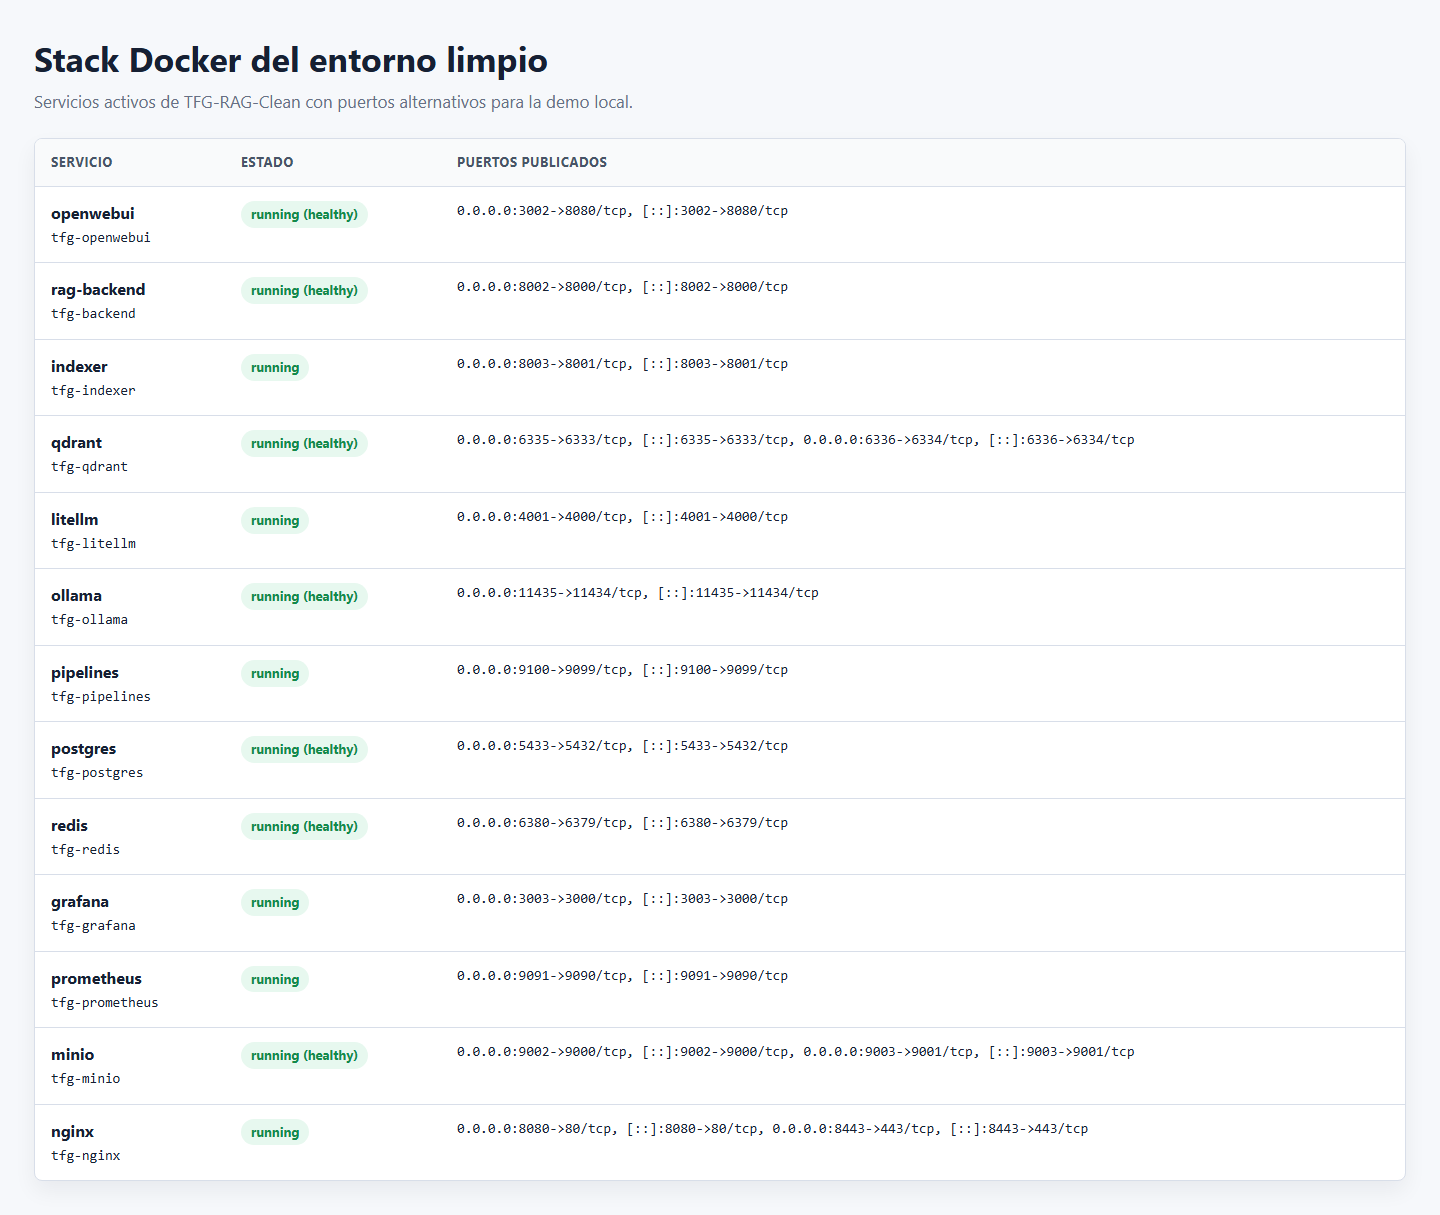
\includegraphics[width=0.95\textwidth]{cap_tfg_docker_stack.png}
\caption{Estado del stack Docker en la validación final. La captura muestra los servicios principales de \texttt{TFG-RAG-Clean}, su estado de ejecución y los puertos alternativos publicados para la demo local.}
\label{fig:docker-stack-final}
\end{figure}

\begin{figure}[H]
\centering
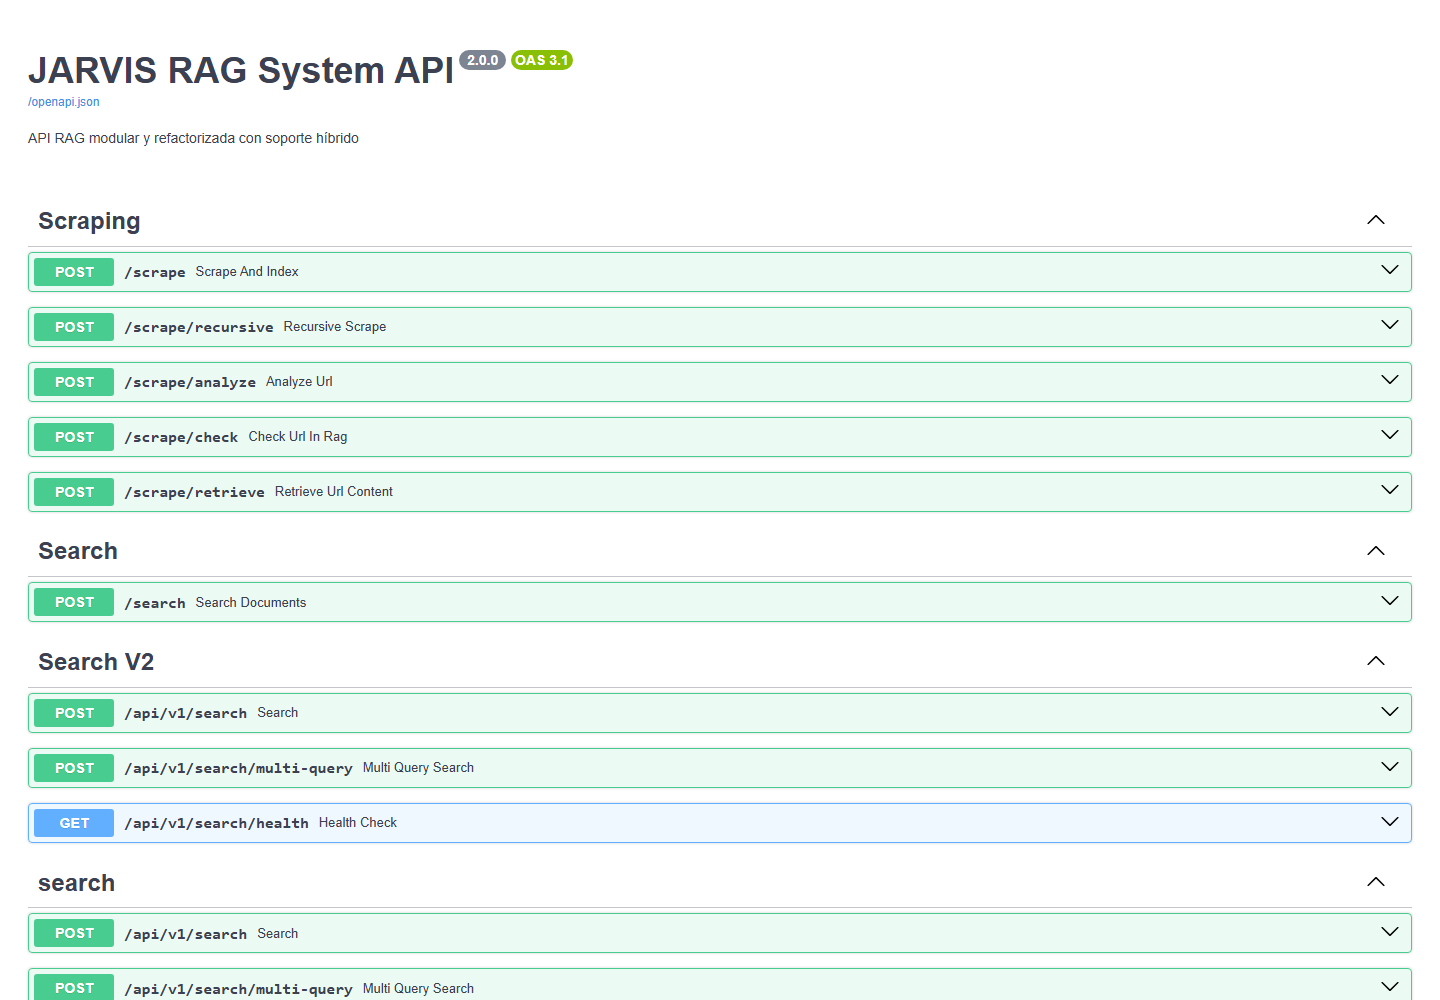
\includegraphics[width=0.9\textwidth]{cap_tfg_backend_swagger.png}
\caption{Documentación interactiva del Backend FastAPI en el entorno local de validación: API activa, endpoints de scraping, búsqueda y salud, y contrato OpenAPI expuesto.}
\label{fig:backend-swagger-final}
\end{figure}

\subsection{Flujo de Datos End-to-End}

Para ilustrar cómo se conectan las piezas, se describe el recorrido completo de una consulta RAG típica:

\begin{enumerate}
    \item El \textbf{usuario} escribe su pregunta en el navegador (OpenWebUI).
    \item \textbf{NGINX} recibe la petición HTTPS y la reenvía internamente a OpenWebUI (puerto 8080).
    \item \textbf{OpenWebUI} envía el mensaje al pipeline JARVIS mediante HTTP POST al puerto 9099.
    \item \textbf{JARVIS} analiza el texto, detecta la intención RAG, obtiene los departamentos autorizados del usuario y construye una petición al Backend.
    \item El \textbf{Backend} genera el embedding de la consulta con SentenceTransformer, ejecuta una búsqueda híbrida en Qdrant y recupera los $k$ fragmentos más relevantes.
    \item El Backend compone un \textit{prompt} estructurado con el contexto recuperado y lo envía a LiteLLM.
    \item \textbf{LiteLLM} verifica si existe una respuesta cacheada en Redis. Si no, delega al modelo en Ollama.
    \item \textbf{Ollama} ejecuta la inferencia en GPU y devuelve los tokens generados en streaming.
    \item La respuesta fluye de vuelta: LiteLLM $\rightarrow$ Backend $\rightarrow$ JARVIS $\rightarrow$ OpenWebUI $\rightarrow$ NGINX $\rightarrow$ navegador.
\end{enumerate}

Todo el flujo se completa típicamente en menos de 3.5 segundos, con el primer token visible para el usuario en menos de 1.2 segundos gracias al streaming.

\begin{figure}[H]
\centering
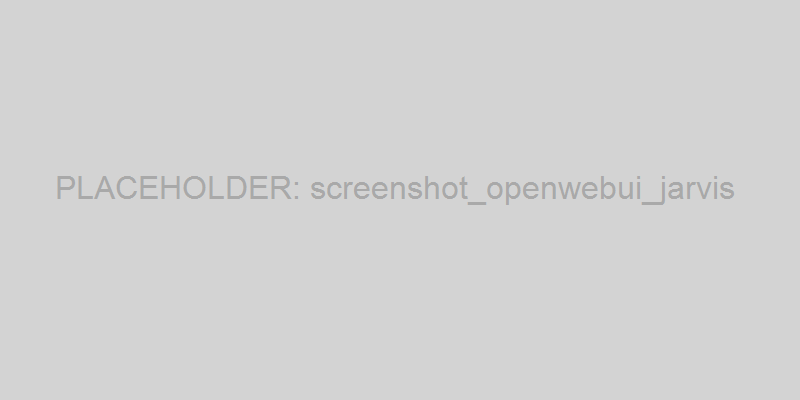
\includegraphics[width=0.85\textwidth]{screenshot_openwebui_jarvis.png}
\caption{Interfaz de OpenWebUI con el modelo JARVIS seleccionado. El usuario escribe su consulta y recibe la respuesta en streaming.}
\label{fig:screenshot-openwebui}
\end{figure}

% ============================================================
\section{Desarrollo Propio vs. Herramientas Externas}
\label{sec:propio-vs-externo}
% ============================================================

Una pregunta fundamental en cualquier proyecto de integración es: ¿qué parte del trabajo es desarrollo original y qué parte es configuración de herramientas existentes? La Tabla~\ref{tab:reuso-desarrollo} clasifica cada componente del sistema según su origen.

\begin{table}[H]
\centering
\caption{Resumen sintético de reutilización y desarrollo dentro del TFG.}
\label{tab:reuso-desarrollo}
\resizebox{\textwidth}{!}{%
\begin{tabular}{p{3.0cm}ccccp{5.2cm}}
\toprule
\textbf{Componente} & \textbf{Reutilizado} & \textbf{Extendido} & \textbf{Desarrollado en el TFG} & \textbf{Integrado} & \textbf{Papel en el sistema} \\
\midrule
OpenWebUI                  & \checkmark & \checkmark & $\times$   & \checkmark & Interfaz conversacional web, persistencia de chats y base para autenticación corporativa. \\
Pipeline JARVIS            & $\times$   & $\times$   & \checkmark & \checkmark & Encaminamiento de intenciones, memoria de sesión y conexión entre interfaz y backend. \\
Backend RAG                & $\times$   & $\times$   & \checkmark & \checkmark & Recuperación documental, scraping, búsqueda web, API BOE y lógica principal del sistema. \\
Indexer                    & $\times$   & $\times$   & \checkmark & \checkmark & Sincronización con SharePoint, OCR e ingesta automatizada de documentos. \\
Ollama y LiteLLM           & \checkmark & \checkmark & $\times$   & \checkmark & Inferencia local, alias de modelos, caché y desacoplo entre servicios y modelos. \\
Qdrant                     & \checkmark & \checkmark & $\times$   & \checkmark & Almacenamiento vectorial y recuperación documental con filtros por colección. \\
Servidor MCP-BOE           & $\times$   & $\times$   & \checkmark & \checkmark & Consulta normativa estructurada y prueba de integración MCP. \\
Prometheus, Grafana y DCGM & \checkmark & \checkmark & $\times$   & \checkmark & Observabilidad operativa del backend, la base de datos y la GPU. \\
\bottomrule
\end{tabular}%
}
\end{table}

En resumen, el trabajo de desarrollo propio abarca más de 6.000 líneas de código Python distribuidas entre el Pipeline JARVIS (1.498 líneas), el Backend ($\sim$3.000), el Indexer ($\sim$1.200) y el servidor MCP-BOE ($\sim$400), además de toda la configuración declarativa del ecosistema Docker (Compose, LiteLLM, NGINX, Prometheus y los dashboards de Grafana). Las herramientas externas proporcionan las capacidades de infraestructura (base de datos, motor LLM, OCR, navegador), pero la lógica de negocio, la orquestación y la inteligencia del sistema son enteramente originales.

% ============================================================
\section[Pipeline de OpenWebUI]{El Mecanismo Pipeline de OpenWebUI (Hook)}
\label{sec:hook-pipeline}
% ============================================================

El Pipeline de OpenWebUI es el punto de conexión fundamental entre la interfaz de usuario y todo el backend del sistema \cite{openwebui2024docs}. Sin este mecanismo, OpenWebUI sería simplemente una interfaz para chatear directamente con Ollama. El Pipeline es lo que convierte esa interfaz genérica en un asistente corporativo inteligente.

En ingeniería de software, un \textit{hook} es un punto de extensión que permite inyectar código personalizado en un flujo de ejecución predefinido sin modificar el sistema original. En OpenWebUI, el \textit{hook} se materializa en el sistema de Pipelines: cuando un usuario envía un mensaje, en lugar de reenviarlo directamente a Ollama, OpenWebUI lo envía primero al servicio Pipeline, que procesa el mensaje, ejecuta la lógica necesaria y devuelve la respuesta. Desde la perspectiva de OpenWebUI, el Pipeline \textit{es} el modelo.

La conexión se establece por configuración: el Pipeline se despliega como contenedor que expone una API HTTP en el puerto 9099, y OpenWebUI se configura con \texttt{OPENAI\_API\_BASE\_URLS} apuntando a él. Al arrancar, OpenWebUI descubre el Pipeline por su nombre (\texttt{JARVIS}) y lo muestra como un modelo seleccionable. El detalle de implementación ---el contrato de la clase \texttt{Pipeline}, el método \texttt{pipe()} con respuesta en \textit{streaming} (\texttt{yield}) y el sistema \textit{Valves} de configuración dinámica desde la interfaz de administración--- se recoge en el Anexo~\ref{anexo:pipeline}.

% ============================================================
\section{Agente Encaminador JARVIS: Inteligencia Central}
\label{sec:jarvis-detalle}
% ============================================================

El agente JARVIS es la pieza de software más compleja del proyecto, con 1.498 líneas de código Python. Su función es analizar cada mensaje del usuario y decidir a cuál de los modos de operación derivarlo. La detección de intenciones se implementa en el método \texttt{\_detect\_intent()}, que evalúa el mensaje contra un conjunto de reglas heurísticas (coincidencia de palabras clave y expresiones regulares) en un \textit{orden de prioridad estricto}: primero las condiciones más específicas (archivos adjuntos, imágenes, URLs) y después las más genéricas (keywords de RAG, búsqueda web, conversación). La Tabla~\ref{tab:intenciones-detalle} resume las categorías, su prioridad y los criterios de activación.

\begin{table}[H]
\centering
\caption{Categorías de intención y su prioridad de evaluación.}
\label{tab:intenciones-detalle}
\begin{tabular}{clp{7cm}}
\toprule
\textbf{Prioridad} & \textbf{Modo} & \textbf{Criterio de activación} \\
\midrule
0 & Decisión pendiente   & Existe una decisión de URL esperando respuesta del usuario \\
1 & Archivo adjunto      & Se detecta un PDF o documento en el cuerpo de la petición \\
2 & Visión/OCR           & Imagen adjunta en el mensaje actual \\
3 & Referencia a imagen  & Mención a ``la imagen'' con imagen previa en memoria \\
4 & Referencia a web     & Mención a ``la web'' o ``la página'' con contenido web en memoria \\
5 & Ayuda                & Keywords: ``qué puedes hacer'', ``ayuda'', ``help'' \\
6 & Listar documentos    & Commands: ``/docs'', ``/listar''; keywords: ``qué documentos tienes'' \\
7 & BOE / Legal          & Keywords: ``busca en el BOE'', ``ley de'', ``real decreto'' \\
8 & RAG Documental       & Keywords: ``documento'', ``política'', ``manual'', ``procedimiento'' \\
9 & URL detectada        & Expresión regular que detecta \texttt{https://...} en el mensaje \\
10 & Búsqueda web        & Keywords: ``busca en internet'', ``noticias'', ``precio'' \\
11 & Estado del sistema  & Keywords: ``cómo va'', ``estado'', ``indexación'' \\
12 & Sticky Mode         & Seguimiento contextual del modo de la pregunta anterior \\
13 & Chat general        & Default: cualquier mensaje que no active otro modo \\
\bottomrule
\end{tabular}
\end{table}

\begin{figure}[H]
\centering
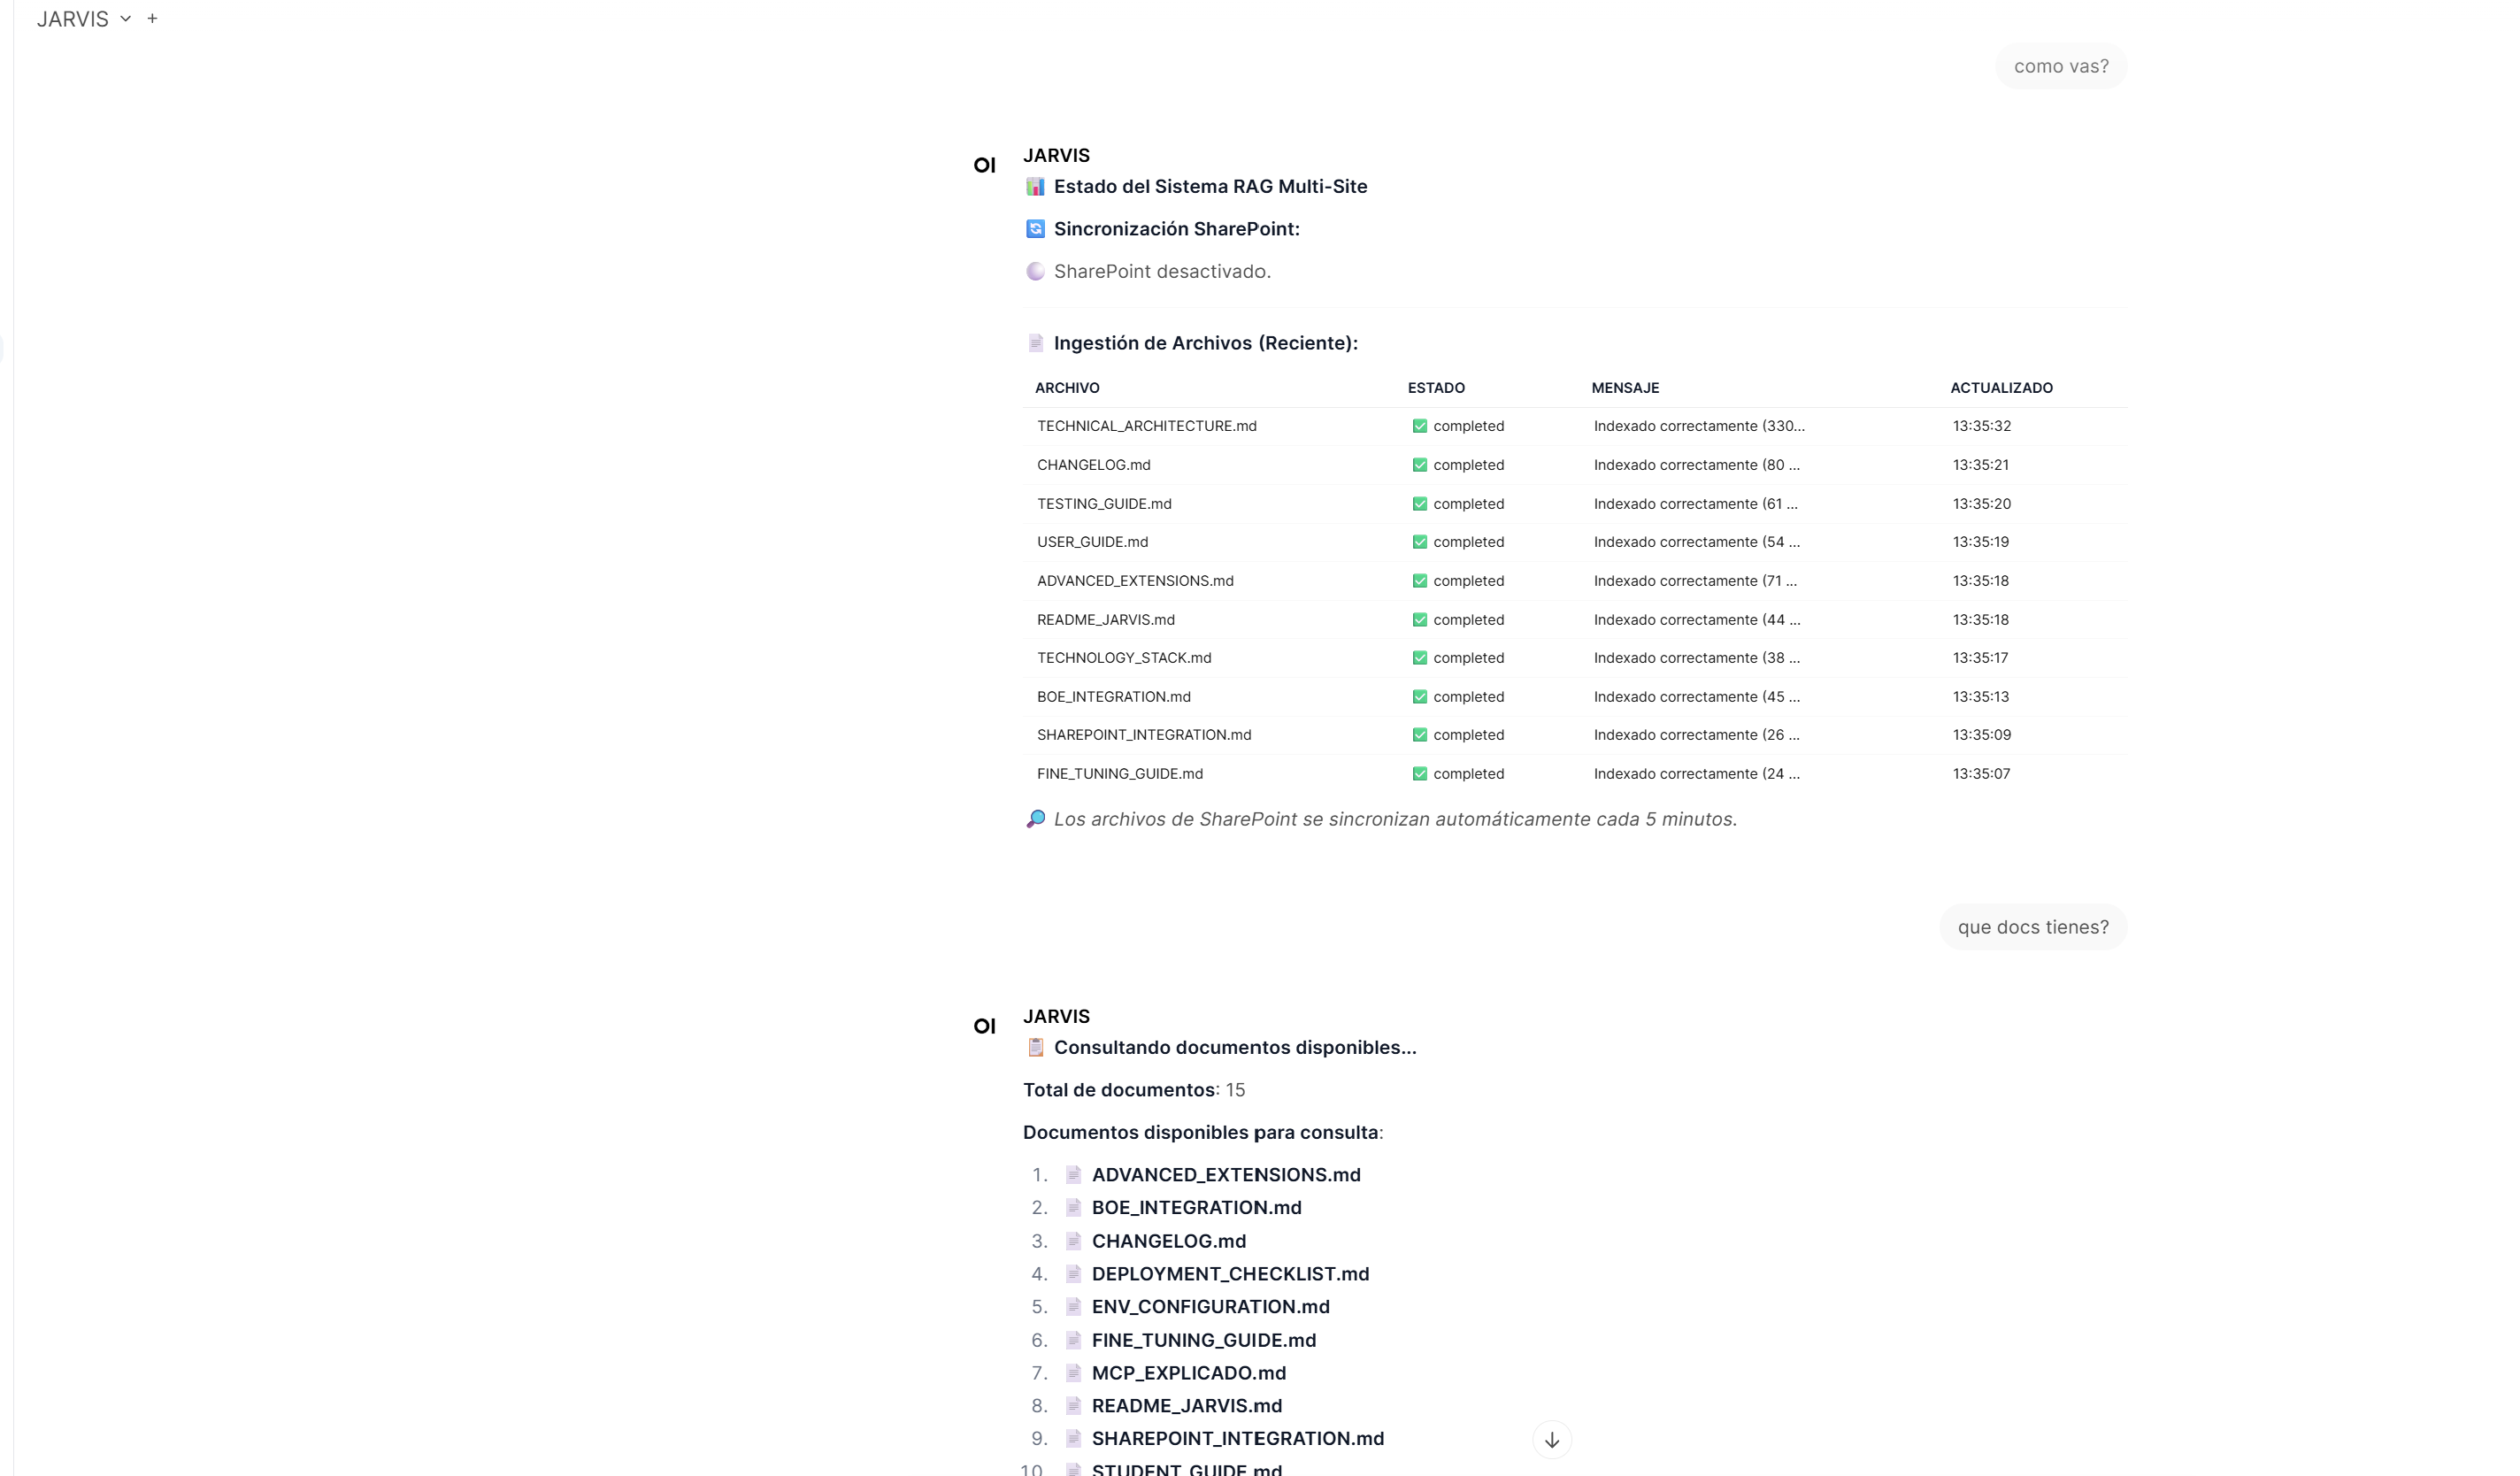
\includegraphics[width=0.85\textwidth]{cap_chat_lista_docs.png}
\caption{Respuesta real del modo de listado documental. JARVIS consulta el estado del indexador y devuelve los documentos disponibles, junto con la información reciente de ingesta.}
\label{fig:documentos-disponibles}
\end{figure}

Más allá del encaminamiento, JARVIS incorpora tres mecanismos de contexto: el \textit{Sticky Mode} (mantiene el modo de la pregunta anterior ante consultas de seguimiento breves y ambiguas), la \textbf{memoria de sesión por usuario} (recuerda la última imagen y la última web analizadas, y gestiona decisiones pendientes) y el \textbf{control de acceso departamental} (mapea los grupos de Azure AD del usuario a colecciones de Qdrant y filtra la búsqueda). El detalle de estos tres mecanismos, con ejemplos de código, se recoge en el Anexo~\ref{anexo:pipeline}.

% ============================================================
\section{Backend RAG: Motor de Búsqueda Semántica}
\label{sec:backend-rag}
% ============================================================

El Backend constituye el motor central de procesamiento del sistema. Implementado en FastAPI, fue objeto de una refactorización significativa: inicialmente era un único fichero \texttt{main.py} de más de 1.900 líneas que se dividió en una arquitectura modular con paquetes separados para esquemas (\texttt{schemas/}), servicios (\texttt{services/}), endpoints (\texttt{api/}), procesamiento (\texttt{processing/}) e integraciones (\texttt{integrations/}).

La \textbf{ingesta} de un documento sigue seis etapas: recepción (API, Indexer o scraper), detección de tipo (texto nativo vs. escaneado), extracción de texto (\texttt{pdfplumber}, PaddleOCR o la cadena Trafilatura/Readability/BeautifulSoup), \textit{chunking} semántico (fragmentos de 512--1024 tokens con 10--15\% de solapamiento), generación de \textit{embeddings} (vector denso de 384 dimensiones con \path{paraphrase-multilingual-MiniLM-L12-v2}) y almacenamiento en Qdrant con metadatos. El procedimiento completo se detalla en el Anexo~\ref{anexo:backend}.

\begin{figure}[H]
\centering
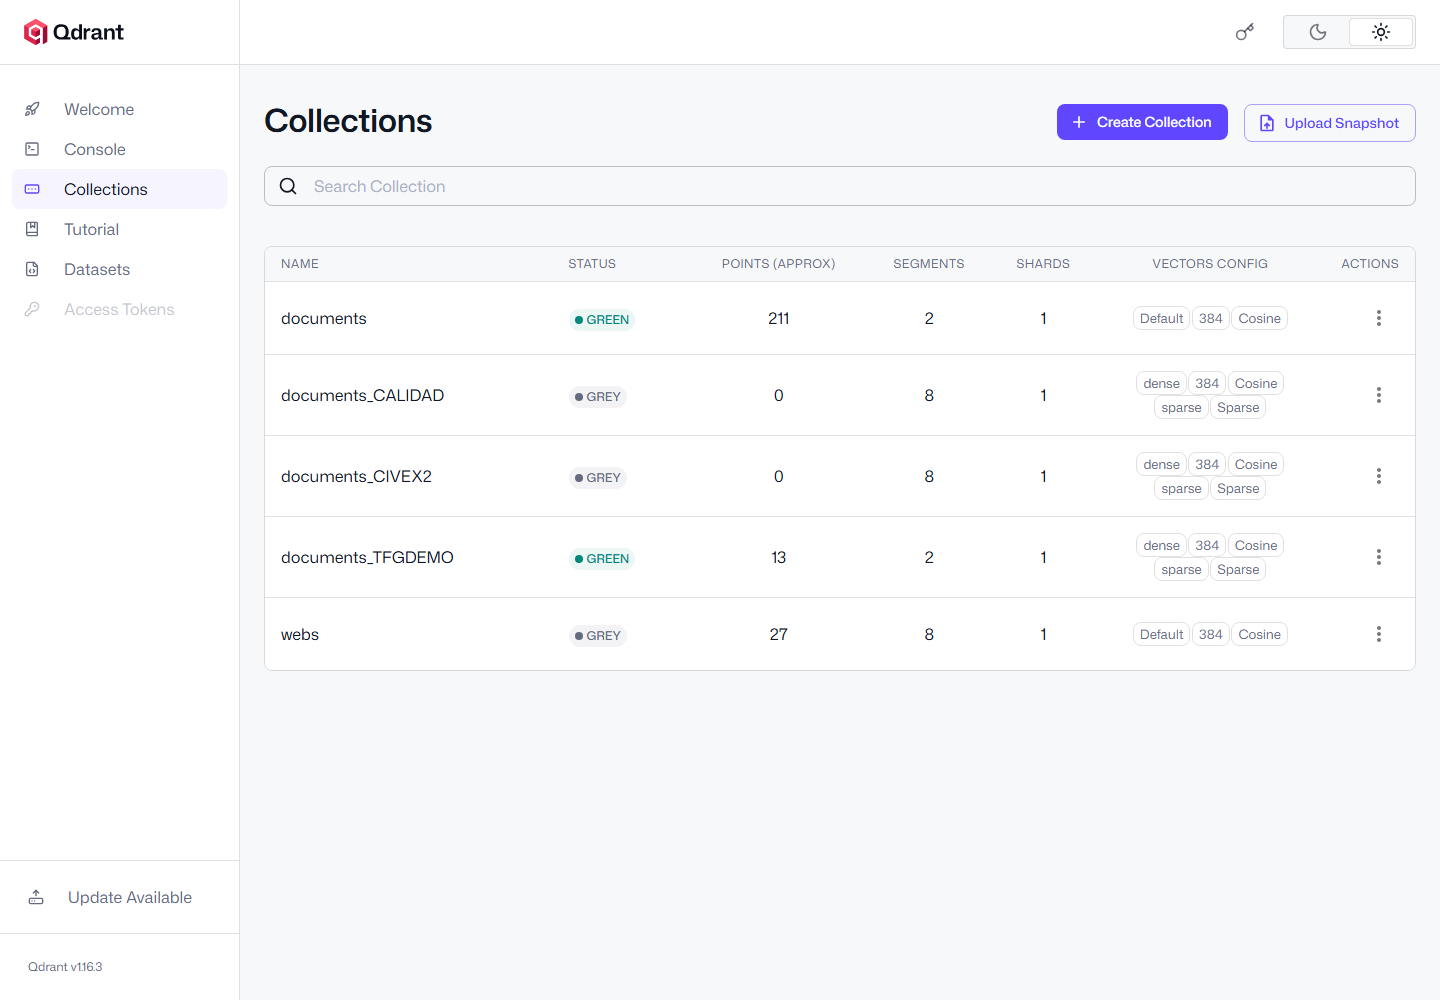
\includegraphics[width=0.9\textwidth]{cap_tfg_qdrant_dashboard.png}
\caption{Estado de las colecciones en Qdrant durante la demo final. La colección \texttt{documents\_TFGDEMO} ---documentación sintética y segura del propio TFG--- aparece separada del resto, con 13 puntos y configuración híbrida dense+sparse.}
\label{fig:qdrant-tfgdemo}
\end{figure}

\subsection{Búsqueda Híbrida}
\label{subsec:busqueda-hibrida}

La recuperación de contexto combina tres etapas complementarias:

\begin{enumerate}
    \item \textbf{Búsqueda densa (HNSW)}: la consulta se transforma en un embedding de 384 dimensiones y se buscan los fragmentos más próximos en el espacio vectorial mediante el índice HNSW de Qdrant.
    \item \textbf{Búsqueda dispersa (BM25)}: se complementa con vectores dispersos generados con \texttt{Qdrant/bm25} (vía \texttt{fastembed}), que favorece coincidencias léxicas exactas ---identificadores, códigos, siglas o artículos legales--- que la búsqueda semántica podría no capturar.
    \item \textbf{Reordenación con reranker}: los candidatos se fusionan y se reordenan con un \textit{Cross-Encoder} (\texttt{cross-encoder/ms-marco-MiniLM-L-6-v2}), que evalúa conjuntamente el par (consulta, fragmento) para obtener una relevancia más precisa antes de seleccionar los $k$ fragmentos finales (típicamente $k=5$).
\end{enumerate}

El \textit{prompt} enviado al LLM combina un \textit{system prompt} restrictivo ---``responde únicamente con el contexto proporcionado, no inventes''--- con una temperatura baja ($0.1$--$0.2$), lo que elimina prácticamente las alucinaciones en modo RAG. La construcción exacta del \textit{prompt} se muestra en el Anexo~\ref{anexo:backend}.

% ============================================================
\section{Extracción Web, OCR e integraciones}
\label{sec:extraccion-integraciones}
% ============================================================

El sistema añade varias fuentes de información más allá de los documentos internos, cuyo detalle de implementación se recoge en los anexos:

\begin{itemize}
    \item \textbf{Scraping y búsqueda web} (Anexo~\ref{anexo:backend}): un motor con Playwright renderiza páginas dinámicas (JavaScript) y una cadena de \textit{fallback} (Trafilatura $\rightarrow$ Readability $\rightarrow$ BeautifulSoup) extrae el contenido principal. La búsqueda en internet usa \texttt{duckduckgo\_search} con \textit{fallback} a scraping HTML.
    \item \textbf{OCR} (Anexo~\ref{anexo:backend}): PaddleOCR con aceleración GPU ---y \textit{fallback} automático a CPU--- procesa los PDFs escaneados, con paralelización mediante Ray durante la ingesta.
    \item \textbf{SharePoint} (Anexo~\ref{anexo:integraciones}): el Indexer sincroniza cada 5 minutos mediante MSAL y Microsoft Graph, con estrategia \textit{delta} incremental para no reprocesar documentos.
\end{itemize}

% ============================================================
\section{Integración con el Boletín Oficial del Estado (BOE)}
\label{sec:boe-impl}
% ============================================================

La integración con el BOE se implementa mediante un servidor MCP (\textit{Model Context Protocol}) construido con \texttt{fastmcp}, que transforma peticiones en lenguaje natural en llamadas estructuradas a la API de Datos Abiertos del BOE. Esta integración no es una búsqueda web genérica, y merece una justificación específica: en el tipo de empresa para la que se diseña el sistema, el acceso a normativa legal (legislación laboral, protección de datos, contratación pública) es frecuente y tiene consecuencias directas. Un error en la interpretación de una norma puede traducirse en incumplimientos o sanciones.

El BOE presenta características que lo distinguen como caso de uso propio: las leyes se identifican por códigos oficiales (p.~ej. \texttt{BOE-A-2018-16673}) y no por títulos que el usuario recuerde; un mismo texto se referencia coloquialmente de muchas formas (``la LOPD'', ``la ley de privacidad''); la información relevante suele estar en artículos numerados concretos; y tanto la exactitud como la fuente son cruciales. Por ello se implementó una capa de resolución semántica que traduce el lenguaje del usuario al identificador normativo correcto antes de invocar la API oficial. El mecanismo de mapeo y la discusión sobre la integración MCP vs.\ API directa se detallan en el Anexo~\ref{anexo:integraciones}.

% ============================================================
\section{Seguridad Perimetral y Autenticación}
\label{sec:seguridad-impl}
% ============================================================

La seguridad del sistema se organiza en capas. \textbf{NGINX} actúa como primera barrera y único servicio expuesto al exterior: termina el TLS (los microservicios internos hablan en texto plano dentro de la red aislada), hace \textit{proxy pass} preservando cabeceras de trazabilidad y habilita el \textit{upgrade} a WebSocket necesario para el streaming. La autenticación de usuarios se delega en \textbf{Azure AD vía OpenID Connect (OIDC)}: los usuarios entran con sus credenciales corporativas y los atributos del token (nombre, correo, grupos) alimentan el control de acceso departamental.

\begin{figure}[H]
\centering
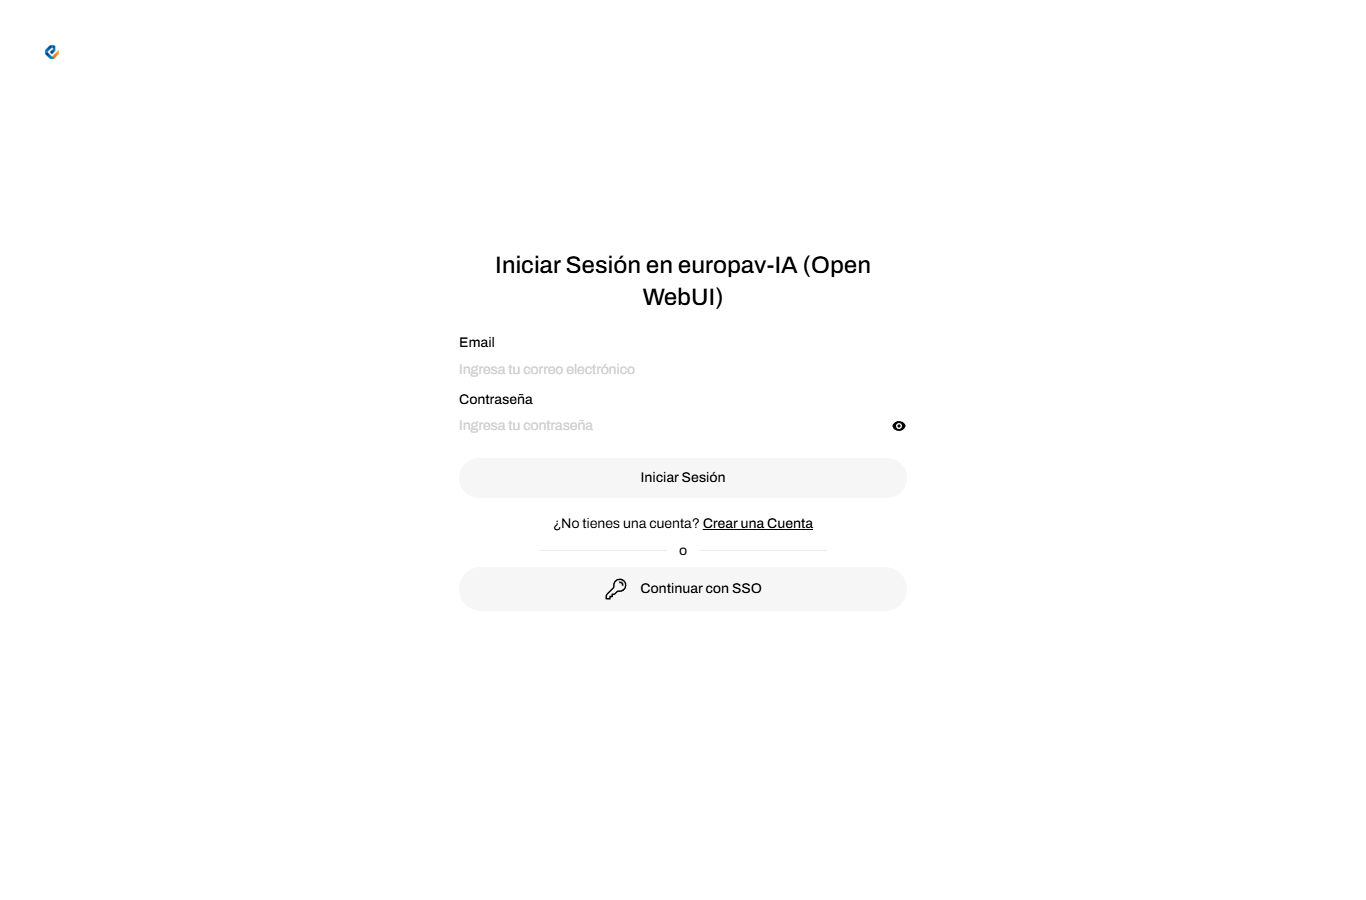
\includegraphics[width=0.85\textwidth]{cap_openwebui_login_actual.png}
\caption{Pantalla real de autenticación de OpenWebUI en el despliegue local: inicio de sesión clásico y acceso mediante SSO corporativo.}
\label{fig:login-sso}
\end{figure}

Además de la autenticación perimetral, el Backend implementa una segunda capa de \textbf{validación criptográfica de tokens JWT} (\texttt{core/auth.py}) para clientes externos y herramientas MCP: descarga las claves públicas JWKS del \textit{tenant}, verifica cada token Bearer y mapea los grupos a colecciones autorizadas, devolviendo \texttt{HTTP 403} si el acceso no es válido. Se activa con \texttt{AZURE\_JWT\_VALIDATION=true}. Finalmente, el \textbf{aislamiento de red} (\texttt{rag-network}, tipo \textit{bridge}) impide el acceso externo directo a PostgreSQL, Redis, Qdrant u Ollama. El flujo JWT paso a paso se detalla en el Anexo~\ref{anexo:integraciones}.

% ============================================================
\section{Observabilidad, caché y almacenamiento}
\label{sec:observabilidad-impl}
% ============================================================

La monitorización respondió a una necesidad real: durante las primeras fases no existía visibilidad sobre el rendimiento, la saturación de la GPU ni los patrones de uso, y la optimización era intuitiva en lugar de basada en datos. El stack adoptado combina \textbf{Prometheus} (métricas del backend: latencias y percentiles, throughput, distribución de modos, errores), \textbf{NVIDIA DCGM Exporter} (VRAM, utilización, temperatura, potencia de la GPU), \textbf{Grafana} (tres dashboards: backend, GPU y base de datos) y \textbf{Loki + Promtail} (agregación de logs de todos los contenedores, consultables junto a las métricas en Grafana) \cite{prometheus2026docs,grafana2026docs,dcgmExporter2026docs}. El detalle de métricas, telemetría y dashboards está en el Anexo~\ref{anexo:integraciones}.

\begin{figure}[H]
\centering
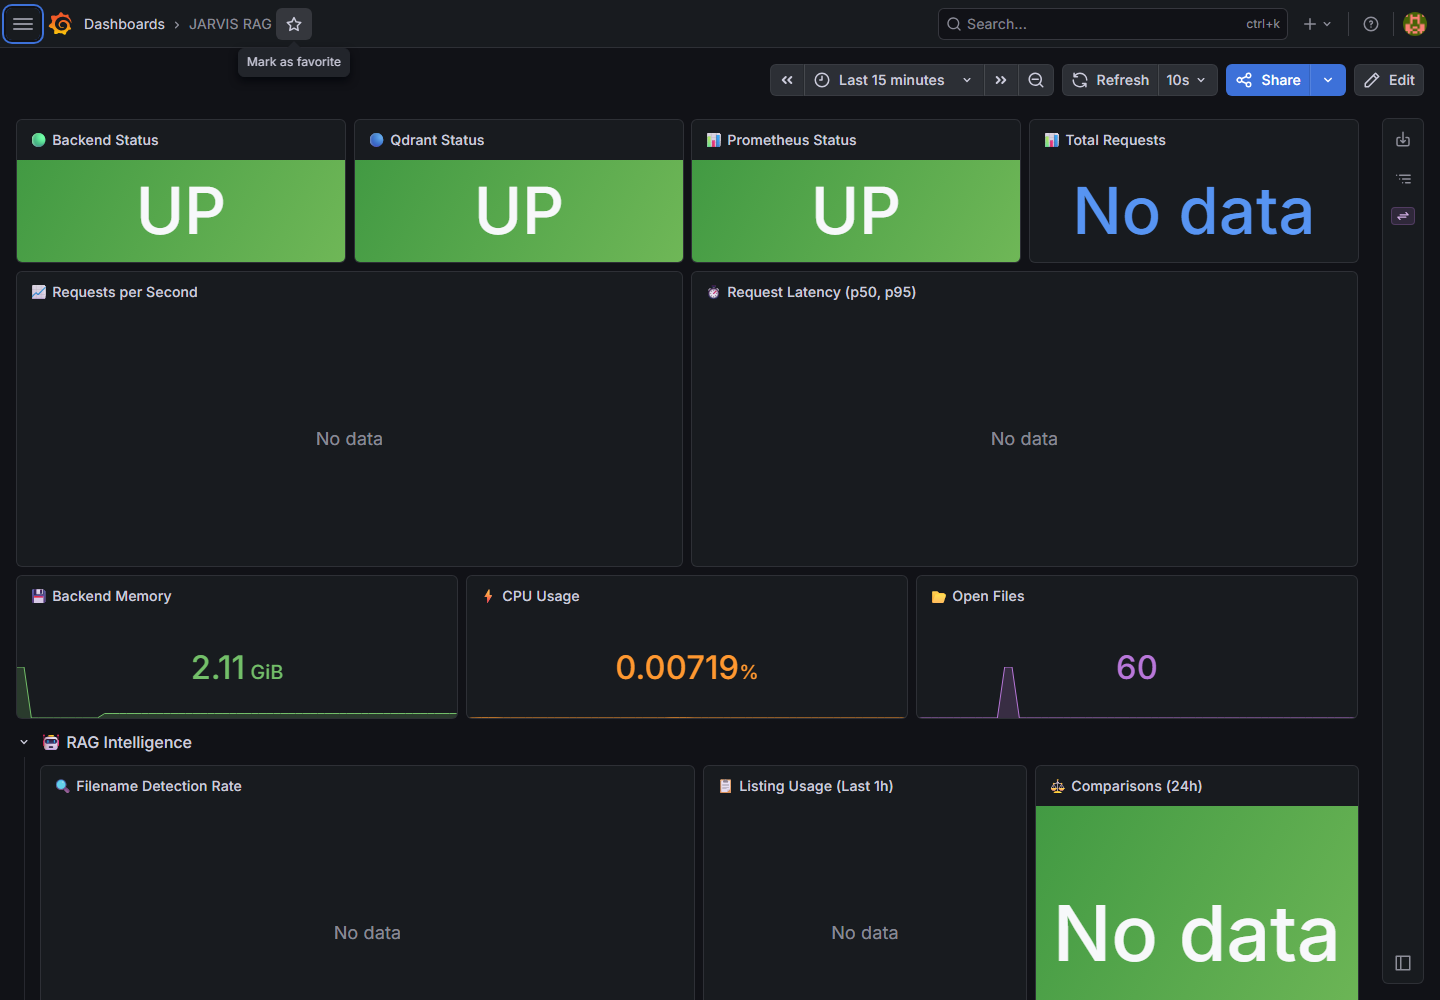
\includegraphics[width=0.9\textwidth]{cap_tfg_grafana_jarvis_dashboard.png}
\caption{Dashboard principal de Grafana durante la validación final: estado operativo del backend, Qdrant y Prometheus, además de métricas de memoria, CPU y ficheros abiertos.}
\label{fig:grafana-final}
\end{figure}

Esta observabilidad condujo a decisiones concretas de optimización: se validó que $\sim$35\% de las consultas repetidas se beneficiaban de la caché, se ajustó el valor de $k$ al detectar que más de 5 fragmentos no mejoraban la respuesta, y se reprogramó la ingesta OCR a horarios de baja actividad al ver que monopolizaba la GPU.

En cuanto al rendimiento y el almacenamiento, \textbf{Redis} actúa como caché integrada con LiteLLM: almacena un hash de cada consulta junto con su respuesta (TTL de 1 hora), con una tasa de aciertos observada de $\sim$35\% que reduce la carga sobre la GPU. \textbf{MinIO} proporciona almacenamiento de objetos compatible con S3 que preserva una réplica aislada de los documentos binarios ingeridos, permitiendo reindexar desde cero sin volver a las fuentes originales (SharePoint, web).

% ============================================================
\section{Agente SQL: Consultas en Lenguaje Natural sobre Datos Estructurados}
\label{sec:sql-agent}
% ============================================================

El pipeline RAG estándar opera solo sobre texto no estructurado, pero muchos sistemas empresariales guardan información crítica en tablas relacionales (métricas, inventarios, datos financieros). Para consultarlas sin saber SQL se desarrolló el agente SQL (\texttt{backend/app/core/sql\_agent.py}), que sigue tres pasos: (1)~\textbf{inspección del esquema} de PostgreSQL para inyectarlo como contexto; (2)~\textbf{generación} de una consulta \texttt{SELECT} con LiteLLM, instruyendo al modelo a producir solo lecturas; y (3)~\textbf{ejecución con auto-corrección}, reintentando con el mensaje de error como contexto (hasta dos veces). La consulta se valida contra una lista blanca (solo \texttt{SELECT}/\texttt{WITH}/\texttt{EXPLAIN}) y se ejecuta con \textit{timeout}; los mecanismos de seguridad se detallan en el Anexo~\ref{anexo:backend}. El endpoint unificado \texttt{POST /api/v1/query} enruta automáticamente entre RAG y SQL según la naturaleza de la consulta, de forma transparente para el usuario.

% ============================================================
\section{Fine-Tuning con LoRA}
\label{sec:finetuning-impl}
% ============================================================

Para adaptar el modelo al dominio corporativo se exploró el ajuste fino con LoRA (\textit{Low-Rank Adaptation}), que inserta matrices de rango reducido en las capas de atención sin modificar los pesos originales, reduciendo los parámetros entrenables a una fracción y haciendo viable el entrenamiento con una sola GPU. El modelo resultante (\texttt{rag-qwen-ft:latest}) es el que sirve de base a JARVIS. El procedimiento completo ---generación del dataset, entrenamiento y evaluación--- se detalla en el Anexo~\ref{anexo:finetuning}.

Una conclusión relevante del proyecto es que, para tareas de RAG puras, el \textit{fine-tuning} del LLM resultó \textit{menos} decisivo que un buen \textit{prompt} restrictivo combinado con una recuperación de calidad (chunking, embeddings, búsqueda híbrida y reranker). El ajuste fino sí aportó valor en la coherencia terminológica y en la adherencia al estilo de respuesta corporativo, pero la inteligencia del sistema descansa sobre todo en la calidad del contexto recuperado, no en la modificación de los pesos del modelo.

\chapter{Proceso de desarrollo del proyecto}
\label{cap:metodologia}

Este capítulo describe cómo se ha construido el proyecto a lo largo del tiempo. Tras situar la organización del código, el grueso del capítulo ---y su verdadero contenido--- es el recorrido \textbf{sprint a sprint}: qué se hizo en cada etapa, qué tecnologías se eligieron frente a qué alternativas y qué lecciones dejó cada una. El balance cuantitativo del proyecto (horas dedicadas, planificación temporal, presupuesto y riesgos) se recoge en el Capítulo~\ref{cap:conclusiones}, junto al resto de conclusiones.

El desarrollo se ha conducido siguiendo un marco de trabajo ágil (\textit{Agile}), caracterizado por entregas iterativas e incrementales. Dada la naturaleza cambiante del ámbito de la Inteligencia Artificial y de los Modelos de Lenguaje Grande (LLMs), la flexibilidad para revisar decisiones técnicas, sustituir herramientas o ajustar el encaminamiento resultó especialmente importante durante el desarrollo.

Se estableció un ciclo de vida con las siguientes fases:
\begin{enumerate}
    \item \textbf{Elicitación y Análisis de Requisitos:} Identificación de fuentes de información clave (SharePoint, páginas web corporativas y el BOE), así como las restricciones de privacidad requeridas por un despliegue puramente \textit{on-premise}.
    \item \textbf{Diseño de Arquitectura:} Planificación de la infraestructura basada en microservicios contenerizados y selección del stack tecnológico idóneo.
    \item \textbf{Implementación Incremental:} Programación progresiva de los módulos de ingesta, OCR, embeddings, búsqueda de Qdrant, backend y, por último, de la interfaz de usuario de OpenWebUI.
    \item \textbf{Pruebas y Validación:} Validación funcional del encaminamiento inteligente y de las capacidades del RAG mediante métricas comparativas empíricas y experimentación cualitativa.
\end{enumerate}

El trabajo se dividió en \textbf{siete sprints} de aproximadamente un mes de duración, desarrollados entre octubre de 2025 y mayo de 2026, a los que siguió una fase final de documentación, redacción de la memoria y difusión del proyecto hasta julio de 2026. Cada sprint se centró en un módulo funcional del sistema y terminó con un entregable operativo. La distribución temporal completa (diagrama de Gantt) y las horas dedicadas a cada sprint se presentan en la Sección~\ref{sec:esfuerzo}.

% ============================================================
\section{Organización del Código}
\label{sec:organizacion-codigo}
% ============================================================

Antes de describir cada sprint conviene tener presente la estructura del repositorio del proyecto, porque cada directorio se corresponde de forma bastante directa con el sprint en el que nació. Esta correspondencia entre organización del código y evolución temporal facilita tanto el mantenimiento como la lectura del historial del proyecto:

\begin{lstlisting}[numbers=none, basicstyle=\ttfamily\footnotesize, caption={Estructura del repositorio y sprint en el que se desarrolló cada componente.}, label={lst:estructura-repo}]
TFG-RAG-URJC/
|-- backend/          <- Servicio FastAPI (sprints 2, 4, 6 y 7)
|   `-- app/          <- api, core (RAG, SQL, QueryProcessor),
|                        integrations, processing, storage...
|-- services/
|   |-- ollama/       <- Motor de inferencia local (sprint 1)
|   |-- litellm/      <- Proxy unificado de modelos (sprint 1)
|   |-- indexer/      <- Sincronizacion SharePoint+OCR (sprint 3)
|   `-- openwebui/    <- Interfaz y pipeline JARVIS (sprint 4)
|-- mcp-boe-server/   <- Servidor MCP del BOE (sprint 5)
|-- scripts/          <- Fine-tuning, datasets, backups (spr. 5)
|-- config/           <- NGINX, Prometheus, Grafana (spr. 1 y 5)
|-- database/         <- Esquema inicial PostgreSQL (sprint 1)
|-- tests/            <- Pruebas del sistema (transversal)
|-- docs/             <- Documentacion tecnica (transversal)
|-- github_pages/     <- Pagina web del proyecto
`-- memoria/          <- Esta memoria (LaTeX)
\end{lstlisting}

% ============================================================
\section{Los Sprints en Detalle}
\label{sec:sprints}
% ============================================================

A continuación se define cada sprint siguiendo un esquema común: descripción y objetivo, tareas realizadas, tecnologías elegidas frente a las alternativas valoradas, y estado final con las lecciones aprendidas. Todos los sprints finalizaron con su entregable operativo, por lo que el estado se detalla junto a las lecciones de cada uno.

\subsection{Sprint 1 (octubre de 2025): Infraestructura base}

\textbf{Descripción.} Construir los cimientos del sistema: la plataforma de contenedores, los servicios de datos y el motor de inferencia local, validando que era viable ejecutar un LLM útil en el hardware disponible.

\textbf{Tareas.} Definición del \texttt{docker-compose} inicial y de la red interna aislada; despliegue de PostgreSQL con su esquema inicial (\texttt{database/init.sql}), Qdrant y Redis; instalación de Ollama con los primeros modelos (Llama 3.1) y del proxy LiteLLM; pruebas de concepto de chat local.

\textbf{Tecnologías y alternativas valoradas.}
\begin{itemize}
    \item \textbf{Ollama} frente a \texttt{llama.cpp} puro o vLLM: Ollama aporta gestión de modelos, carga/descarga automática de VRAM y una API estable con mínima configuración. vLLM ofrece mayor rendimiento bruto, pero está orientado a servir un único modelo de forma intensiva; aquí se necesitaba rotar varios modelos sobre una sola GPU.
    \item \textbf{Qdrant} frente a pgvector, Chroma o Pinecone: se buscaba una base vectorial \textit{on-premise} con índice HNSW, colecciones separadas y filtrado por metadatos (la base del control de acceso por departamento). Pinecone se descartó por ser un servicio en la nube, contrario al requisito de soberanía del dato.
    \item \textbf{Docker Compose} frente a Kubernetes: para un despliegue de nodo único, Kubernetes añadía complejidad operativa sin beneficio real.
\end{itemize}

\textbf{Estado y lecciones.} Completado. La lección central llegó ya en este sprint: la GPU es un recurso compartido y escaso, y esa restricción condicionó todas las decisiones posteriores (cuantización, modelos de embeddings en CPU, carga bajo demanda).

\subsection{Sprint 2 (noviembre de 2025): Backend y pipeline RAG}

\textbf{Descripción.} Desarrollar el motor del sistema: un backend propio con el pipeline RAG completo, desde la ingesta del documento hasta la respuesta con citas.

\textbf{Tareas.} API REST con FastAPI; ingesta de PDFs con \texttt{pdfplumber}; \textit{chunking} con solapamiento (500 tokens, solapamiento de 50); generación de embeddings con \path{paraphrase-multilingual-MiniLM-L12-v2} en CPU; búsqueda semántica en Qdrant; construcción del prompt restrictivo con citas de fuente y página.

\textbf{Tecnologías y alternativas valoradas.}
\begin{itemize}
    \item \textbf{FastAPI} frente a Flask o Django: asincronía nativa (esencial para no bloquear durante inferencias largas), validación con Pydantic y documentación OpenAPI generada automáticamente.
    \item \textbf{Pipeline RAG propio} frente a LangChain o LlamaIndex: los \textit{frameworks} aceleran el prototipo, pero ocultan los pasos intermedios. Implementar el pipeline a mano dio control fino sobre chunking, búsqueda y prompt, y sobre todo trazabilidad completa para depurar; esa comprensión del flujo es además parte del valor académico del trabajo.
    \item \textbf{Embeddings en CPU} frente a GPU: el modelo MiniLM es lo bastante ligero para ejecutarse en CPU, reservando la VRAM para los modelos generativos.
\end{itemize}

\textbf{Estado y lecciones.} Completado. La calidad del RAG depende tanto de la ingesta (tamaño de fragmento, solapamiento, limpieza) como del propio modelo generativo: gran parte de las mejoras posteriores vinieron de recuperar mejor, no de generar mejor.

\subsection{Sprint 3 (diciembre de 2025): SharePoint y OCR}

\textbf{Descripción.} Conectar el sistema a las fuentes documentales corporativas reales: la biblioteca SharePoint de la organización y los documentos escaneados.

\textbf{Tareas.} Servicio Indexer con sincronización periódica (cron cada 5 minutos); autenticación MSAL con flujo de credenciales de cliente y descarga incremental vía Microsoft Graph API; motor OCR PaddleOCR con aceleración GPU y \textit{fallback} automático a CPU; paralelización del OCR con Ray.

\textbf{Tecnologías y alternativas valoradas.}
\begin{itemize}
    \item \textbf{PaddleOCR} frente a Tesseract: mejor precisión sobre los documentos escaneados reales del entorno de validación y soporte GPU nativo.
    \item \textbf{Sondeo incremental} frente a \textit{webhooks} de Graph: los webhooks exigen exponer un endpoint público accesible desde Microsoft, incompatible con un despliegue cerrado; el sondeo cada pocos minutos resultó suficiente para la frecuencia de cambio real de los documentos.
\end{itemize}

\textbf{Estado y lecciones.} Completado. Al paralelizar la ingesta apareció una \textit{race condition} en la generación de embeddings que hubo que serializar; y quedó claro que las fuentes corporativas cambian constantemente, lo que convirtió la sincronización incremental en pieza central del diseño.

\subsection{Sprint 4 (enero de 2026): Agente JARVIS, scraping y búsqueda web}

\textbf{Descripción.} Dar al sistema su cara visible y sus capacidades web: el pipeline JARVIS sobre OpenWebUI, que enruta cada consulta al modo adecuado, y la extracción de contenido de internet.

\textbf{Tareas.} Desarrollo del pipeline JARVIS como \textit{hook} de OpenWebUI con detección de intenciones por reglas y sistema de \textit{valves} de configuración; scraping con Playwright (renderizado JavaScript completo) y cadena de extracción Trafilatura $\rightarrow$ Readability $\rightarrow$ BeautifulSoup; búsqueda en internet con DuckDuckGo.

\textbf{Tecnologías y alternativas valoradas.}
\begin{itemize}
    \item \textbf{OpenWebUI con pipeline propio} frente a interfaz web desarrollada desde cero: OpenWebUI ya resuelve autenticación, historial, streaming y gestión de usuarios; el valor diferencial estaba en la lógica de enrutamiento, no en reconstruir un chat.
    \item \textbf{Playwright} frente a peticiones HTTP con BeautifulSoup: gran parte de las páginas corporativas y de noticias actuales requieren ejecutar JavaScript para mostrar su contenido.
    \item \textbf{Router por reglas} frente a un LLM decisor: las reglas son instantáneas, gratuitas y deterministas, y el modelo local desplegado no ofrecía \textit{function calling} fiable. Esta decisión se analiza en detalle en el Capítulo~\ref{cap:implementacion}.
\end{itemize}

\textbf{Estado y lecciones.} Completado. Dos incidencias de despliegue dejaron lección: un pipeline duplicado por el mecanismo de descubrimiento de OpenWebUI y un script de inicialización de Ollama roto por los finales de línea CRLF al editar desde Windows; ambas reforzaron la necesidad de probar el despliegue completo desde cero, no solo el código.

\subsection{Sprint 5 (febrero de 2026): BOE, \textit{fine-tuning} y observabilidad}

\textbf{Descripción.} Ampliar el sistema en tres frentes: la fuente normativa oficial (BOE), la adaptación del modelo al dominio mediante \textit{fine-tuning} y la monitorización del conjunto.

\textbf{Tareas.} Servidor MCP del BOE e integración funcional por API; generación de un dataset sintético de preguntas y respuestas a partir de los documentos indexados en Qdrant; entrenamiento de un adaptador LoRA (PEFT, bitsandbytes, TRL) que dio lugar a \texttt{rag-qwen-ft}, el modelo JARVIS; despliegue del stack de observabilidad (Prometheus, Grafana, exportador DCGM para GPU, y posteriormente Loki y Promtail para logs).

\textbf{Tecnologías y alternativas valoradas.}
\begin{itemize}
    \item \textbf{LoRA} frente a \textit{fine-tuning} completo: ajustar todos los pesos de un modelo de 7B parámetros excede la VRAM disponible; LoRA entrena una fracción mínima de parámetros con resultados comparables para adaptación de dominio.
    \item \textbf{MCP} frente a integración directa por API: se implementaron ambas. MCP se adoptó como apuesta de estandarización futura, pero la interfaz web principal no lo soporta de forma nativa, por lo que la vía de producción siguió siendo la API (la valoración completa está en el Anexo~\ref{anexo:integraciones}).
    \item \textbf{Prometheus y Grafana} frente a soluciones de monitorización en la nube: coherencia con el requisito \textit{on-premise} del proyecto.
\end{itemize}

\textbf{Estado y lecciones.} Completado. La lección más importante de todo el proyecto salió de aquí: el \textit{fine-tuning} rindió resultados modestos para RAG, mientras que las mejoras de recuperación (búsqueda híbrida y reranking) tuvieron un impacto muy superior. Esto reorientó el esfuerzo restante hacia la calidad de la recuperación.

\subsection{Sprint 6 (marzo--abril de 2026): Agente SQL, seguridad y v2.2.0}

\textbf{Descripción.} Incorporar la consulta de datos estructurados en lenguaje natural y endurecer la seguridad del sistema, además de corregir defectos detectados en producción.

\textbf{Tareas.} Agente NL$\rightarrow$SQL sobre PostgreSQL con lista blanca de operaciones (\texttt{SELECT}) y auto-corrección ante errores; validación de tokens JWT de Azure AD contra JWKS en el backend; diagnóstico y corrección de la expansión de consultas asíncrona (versión 2.2.0).

\textbf{Tecnologías y alternativas valoradas.}
\begin{itemize}
    \item \textbf{Validación por lista blanca y expresiones regulares} frente a confiar en las instrucciones del prompt: un LLM puede ser inducido a generar SQL destructivo; la validación programática actúa como defensa en profundidad independiente del modelo.
    \item \textbf{Validación JWT en el backend} frente a delegar la autenticación en la interfaz: cada microservicio verifica la identidad por sí mismo, de modo que un fallo en la capa de presentación no expone los datos.
\end{itemize}

\textbf{Estado y lecciones.} Completado. La incidencia más formativa: la expansión de consultas llevaba tiempo desactivada por un defecto de configuración sin que ninguna prueba lo detectara. La lección es que los tests deben cubrir también la configuración efectiva del sistema en ejecución, no solo la lógica del código.

\subsection{Sprint 7 (mayo de 2026): QueryProcessor y v2.3.0}

\textbf{Descripción.} Cerrar el sistema con la capa de orquestación inteligente: decidir, para cada consulta, qué modelo y qué estrategia de recuperación usar.

\textbf{Tareas.} Módulo \texttt{QueryProcessor} con detección de intención, encaminamiento inteligente entre modelos (JARVIS para consultas factuales y procedimentales; Qwen 2.5 32B para las analíticas) y expansión de consultas multivariante; summarización del historial de conversación con el modelo de 32B en el \texttt{MemoryManager} (versión 2.3.0).

\textbf{Tecnologías y alternativas valoradas.}
\begin{itemize}
    \item \textbf{Encaminamiento por intención entre dos modelos} frente a usar siempre el modelo mayor: las pruebas comparativas mostraron que el modelo ajustado de 7B domina en recuperación precisa con citas mientras que el de 32B destaca en razonamiento analítico; usar cada uno donde sobresale mejora calidad y latencia a la vez.
\end{itemize}

\textbf{Estado y lecciones.} Completado. El modelo más grande no siempre es la mejor opción: adaptar la elección del modelo a la intención de la consulta resultó más eficiente que cualquier elección fija.

\chapter{Resultados y Evaluación}
\label{cap:resultados}

Este capítulo presenta los resultados obtenidos tras el despliegue del sistema en un entorno real. Se analizan las métricas de rendimiento recopiladas por el stack de observabilidad, se describen las pruebas funcionales realizadas sobre cada modo de operación y se valora cualitativamente la calidad de las respuestas del sistema.

% ============================================================
\section{Métricas de Rendimiento}
% ============================================================

El sistema se sometió a pruebas de rendimiento sostenidas en un entorno real durante un período de 30 días. Además, las métricas se recopilaron automáticamente mediante la integración con Prometheus y los paneles configurados en Grafana \cite{prometheus2026docs,grafana2026docs}. La Tabla~\ref{tab:metricas-resultado} sintetiza los indicadores principales.

\begin{table}[H]
\centering
\caption{Métricas de rendimiento del sistema en producción.}
\label{tab:metricas-resultado}
\begin{tabular}{lc}
\toprule
\textbf{Métrica} & \textbf{Valor} \\
\midrule
Tiempo hasta primer token (TTFT) & $< 1.2$~s \\
Latencia RAG completa (p95)       & $\sim 3.5$~s \\
Throughput máximo sostenido       & $\sim 42$ req/min \\
Uptime del sistema                & 99.8\% (30 días) \\
Consumo VRAM pico (3 modelos)     & 18.5 / 24 GB \\
Alucinaciones en modo RAG         & 0\% (temp $\leq$ 0.2) \\
Cache hit rate (Redis)            & $\sim 35$\% \\
\bottomrule
\end{tabular}
\end{table}

\subsection{Análisis de Latencia}

La latencia del sistema se descompone en los siguientes segmentos:

\begin{table}[H]
\centering
\caption{Desglose de latencia por componente para una consulta RAG típica.}
\label{tab:latencia-desglose}
\begin{tabular}{lc}
\toprule
\textbf{Componente} & \textbf{Tiempo} \\
\midrule
NGINX + OpenWebUI $\rightarrow$ Pipeline  & $\sim 50$~ms \\
Detección de intención en JARVIS          & $\sim 10$~ms \\
Generación de embedding (CPU)             & $\sim 80$~ms \\
Búsqueda en Qdrant (top-5)               & $\sim 30$~ms \\
Composición del prompt                    & $\sim 5$~ms \\
Inferencia LLM (primer token)            & $\sim 800$~ms \\
Generación completa (streaming)           & $\sim 2.500$~ms \\
\midrule
\textbf{Total}                            & $\sim 3.475$~ms \\
\bottomrule
\end{tabular}
\end{table}

El cuello de botella principal es la inferencia del LLM en GPU, que representa más del 90\% del tiempo total. Sin embargo, gracias al streaming, el usuario percibe el primer token en aproximadamente 1.2 segundos, lo que proporciona una experiencia de respuesta instantánea. La Figura~\ref{fig:latencia-barras} representa gráficamente esta descomposición.

\begin{figure}[H]
\centering
\begin{tikzpicture}
\begin{axis}[
    xbar,
    width=0.82\textwidth,
    height=7.5cm,
    xlabel={Tiempo (ms)},
    symbolic y coords={
        {NGINX + OpenWebUI},
        {Detección de intención},
        {Embedding (CPU)},
        {Búsqueda Qdrant},
        {Composición prompt},
        {Inferencia LLM (1er token)},
        {Generación completa}
    },
    ytick=data,
    y tick label style={font=\footnotesize, anchor=east},
    x tick label style={font=\footnotesize},
    nodes near coords,
    nodes near coords style={font=\scriptsize},
    bar width=10pt,
    xmin=0,
    xmax=3000,
    enlarge y limits=0.12,
    every axis plot/.append style={fill=blue!35, draw=blue!60},
]
\addplot coordinates {
    (50,{NGINX + OpenWebUI})
    (10,{Detección de intención})
    (80,{Embedding (CPU)})
    (30,{Búsqueda Qdrant})
    (5,{Composición prompt})
    (800,{Inferencia LLM (1er token)})
    (2500,{Generación completa})
};
\end{axis}
\end{tikzpicture}
\caption{Descomposición de la latencia por componente para una consulta RAG típica. La inferencia del LLM domina el tiempo total del flujo.}
\label{fig:latencia-barras}
\end{figure}

\subsection{Gestión de VRAM}

La GPU NVIDIA con 24 GB de VRAM constituye el recurso más crítico del sistema. La Tabla~\ref{tab:vram-modelos} muestra el consumo de VRAM de cada modelo y las combinaciones viables de carga simultánea:

\begin{table}[H]
\centering
\small
\caption{Consumo de VRAM por modelo y combinaciones de carga simultánea.}
\label{tab:vram-modelos}
\begin{tabularx}{\textwidth}{>{\raggedright\arraybackslash}p{4.8cm} c >{\raggedright\arraybackslash}X}
\toprule
\textbf{Modelo} & \textbf{VRAM} & \textbf{Coexistencia} \\
\midrule
JARVIS (\texttt{rag-qwen-ft:latest})        & $\sim 8$ GB & Sí, con servicios auxiliares y modelos ligeros \\
Qwen 2.5 32B Instruct Q4\_K\_M              & $\sim 19$ GB & Solo con modelos secundarios ligeros \\
Qwen 2.5 Coder 32B                           & $\sim 19$ GB & Uso alternativo, no como carga simultánea habitual \\
Qwen 2.5 VL 7B                               & $\sim 6$ GB & Sí \\
PaddleOCR                      & $\sim 500$ MB & Sí \\
\midrule
\textbf{Pico observado} & $\sim 20$ GB & --- \\
\bottomrule
\end{tabularx}
\end{table}

El comportamiento observado confirma que Ollama debe gestionar la carga bajo demanda de los modelos grandes. En el despliegue actual, el alias principal JARVIS se apoya en \texttt{rag-qwen-ft:latest}, mientras que \texttt{qwen2.5:32b-instruct-q4\_K\_M} queda disponible como modelo de texto alternativo.

% ============================================================
\section{Evaluación Funcional}
% ============================================================

Se realizaron pruebas funcionales sistemáticas sobre cada modo de operación del sistema. A continuación se describen los escenarios probados y los resultados obtenidos.

\subsection{Consulta RAG sobre Documentos Corporativos}

\begin{itemize}
    \item \textbf{Prueba:} ``¿Cuál es la política de calidad de la empresa?''
    \item \textbf{Resultado:} El sistema recuperó correctamente los fragmentos más relevantes del manual de calidad indexado y generó una respuesta estructurada con referencias a las secciones y páginas del documento original.
    \item \textbf{Calidad:} La respuesta se fundamentó exclusivamente en el contenido del documento, sin añadir información no presente en los fragmentos recuperados. La temperatura baja ($0.1$) impidió cualquier generación creativa no deseada.
\end{itemize}

\subsection{Scraping de URL}

\begin{itemize}
    \item \textbf{Prueba:} Envío de una URL de documentación técnica de Docker junto con la pregunta ``¿Qué opciones de GPU existen?''
    \item \textbf{Resultado:} El sistema renderizó la página con Playwright y extrajo el contenido con Trafilatura \cite{playwright2024docs,barbaresi2021trafilatura}, generando una respuesta centrada en las opciones de GPU, con citas al texto extraído.
    \item \textbf{Calidad:} La extracción fue precisa incluso en páginas con carga diferida de JavaScript. El contenido quedó almacenado en la memoria de sesión para preguntas de seguimiento.
\end{itemize}

\subsection{Búsqueda Legal en el BOE}

\begin{itemize}
    \item \textbf{Prueba:} ``Busca en el BOE la ley de protección de datos''
    \item \textbf{Resultado:} El sistema resolvió semánticamente ``ley de protección de datos'' al identificador oficial BOE-A-2018-16673, consultó la API del BOE y devolvió un resumen estructurado con título, fecha de publicación y extracto del contenido.
    \item \textbf{Calidad:} La resolución semántica funcionó correctamente para las leyes incluidas en el diccionario de mapeos.
\end{itemize}

\subsection{Análisis de Imagen}

\begin{itemize}
    \item \textbf{Prueba:} Adjuntar una fotografía de un documento en papel y preguntar ``¿Qué pone en este documento?''
    \item \textbf{Resultado:} El modelo de visión (Qwen 2.5 VL) identificó correctamente el texto visible en la imagen y generó una transcripción del contenido.
    \item \textbf{Calidad:} Satisfactoria para documentos con texto legible. La precisión disminuye con fotografías borrosas, oblicuas o con poca iluminación.
\end{itemize}

\subsection{Consultas NL$\rightarrow$SQL con el Agente SQL}

\begin{itemize}
    \item \textbf{Prueba:} ``¿Cuántos documentos han sido indexados esta semana?''
    \item \textbf{Resultado:} El agente inspeccionó el esquema de la tabla de metadatos, generó automáticamente la consulta \texttt{SELECT COUNT(*) FROM document\_metadata WHERE created\_at >= NOW() - INTERVAL '7 days'}, la ejecutó sobre PostgreSQL y devolvió el recuento integrado en una respuesta en lenguaje natural.
    \item \textbf{Calidad:} Correcta en 8 de 10 consultas de prueba. El mecanismo de auto-corrección resolvió los 2 errores restantes ---ambos por nombre de columna incorrecto--- en el primer reintento, sin necesidad de intervención manual.
\end{itemize}

\begin{itemize}
    \item \textbf{Prueba (seguridad):} Intento de inyectar \texttt{DROP TABLE document\_metadata} encubierto como pregunta natural.
    \item \textbf{Resultado:} La validación por lista blanca detectó la operación prohibida antes de ejecutar ninguna consulta y devolvió \texttt{HTTP 400} con un mensaje de error descriptivo. La tabla permaneció intacta.
    \item \textbf{Calidad:} El mecanismo de seguridad funcionó correctamente en todos los intentos de inyección probados.
\end{itemize}

\subsection{Encaminamiento Inteligente}

Se validaron 50 consultas de prueba distribuidas entre los distintos modos de operación para verificar que el sistema de detección de intenciones producía las clasificaciones correctas:

\begin{table}[H]
\centering
\caption{Resultados de la evaluación del encaminamiento de JARVIS.}
\label{tab:enrutamiento-eval}
\begin{tabular}{lcc}
\toprule
\textbf{Modo esperado} & \textbf{Aciertos / Total} & \textbf{Precisión} \\
\midrule
RAG           & 10 / 10 & 100\% \\
Web Search    & 8 / 10  & 80\% \\
Web Scraping  & 10 / 10 & 100\% \\
Visión/OCR    & 5 / 5   & 100\% \\
BOE           & 5 / 5   & 100\% \\
Chat general  & 8 / 10  & 80\% \\
\midrule
\textbf{Total} & \textbf{46 / 50} & \textbf{92\%} \\
\bottomrule
\end{tabular}
\end{table}

Los 4 errores de clasificación ocurrieron en consultas ambiguas donde los keywords de web search se solapaban con los de chat general (ej: ``¿qué es Docker?'' clasificado como web search en lugar de chat). Estos casos edge se consideraron aceptables dado que la respuesta del sistema sigue siendo relevante independientemente del modo seleccionado.

% ============================================================
\section{Mitigación de Alucinaciones}
% ============================================================

La eliminación de alucinaciones en modo RAG se logró mediante la combinación de tres técnicas complementarias:

\begin{enumerate}
    \item \textbf{Temperatura determinista:} Los parámetros de inferencia se configuraron con valores de temperatura entre $0.1$ y $0.2$ en modo RAG, minimizando la aleatoriedad en la selección de tokens.

    \item \textbf{Prompt de sistema restrictivo:} El \textit{system prompt} inyectado instruye explícitamente al modelo para que responda \textbf{únicamente} basándose en el contexto recuperado, prohibiendo la generación libre de información no respaldada por los fragmentos.

    \item \textbf{Solapamiento de ventanas contextuales:} El solapamiento del 10--15\% en el chunking asegura que el hilo semántico de párrafos extensos no se pierde en los límites de fragmento, proporcionando al modelo contexto suficiente para generar respuestas coherentes.
\end{enumerate}

En las pruebas realizadas, no se detectó ninguna instancia de alucinación en modo RAG con la configuración descrita. El modelo respondió ``No dispongo de esa información en los documentos consultados'' cuando la pregunta no encontraba coincidencias relevantes en Qdrant, que es el comportamiento deseado.

% ============================================================
\section{Impacto de la Caché}
% ============================================================

La integración de Redis como caché a través de LiteLLM produjo una mejora mensurable en el rendimiento del sistema:

\begin{itemize}
    \item \textbf{Cache hit rate:} $\sim 35$\% de las consultas se resolvieron directamente desde caché.
    \item \textbf{Reducción de carga GPU:} Las consultas cacheadas no invocan a Ollama, liberando la GPU para nuevas peticiones.
    \item \textbf{Latencia de respuesta cacheada:} $< 100$~ms frente a $\sim 3.5$~s de una consulta RAG completa.
\end{itemize}

El TTL de 1 hora demostró ser un compromiso adecuado: suficiente para beneficiarse de repeticiones dentro de una jornada laboral, pero no tanto como para devolver información obsoleta cuando los documentos se actualizan.

\chapter{Conclusiones y Trabajo Futuro}
\label{cap:conclusiones}

Este capítulo cierra la memoria haciendo balance del trabajo: qué se ha conseguido y con qué medios, cuánto esfuerzo ha requerido, qué conocimientos ---del grado y adquiridos por cuenta propia--- lo han hecho posible, qué lecciones deja y hacia dónde puede evolucionar. Al final del capítulo se recogen las direcciones públicas del código y de la página web del proyecto.

% ============================================================
\section{Resumen General}
% ============================================================

Este Trabajo de Fin de Grado ha permitido diseñar, desarrollar y desplegar un asistente corporativo basado en RAG ejecutado en infraestructura local. El resultado no es un nuevo modelo entrenado desde cero, sino un sistema completo que reutiliza modelos y herramientas existentes y los integra dentro de una arquitectura propia orientada a un problema concreto: consultar documentación corporativa cambiante de forma segura, comprensible y trazable.

La solución obtenida demuestra que es viable construir una capa conversacional útil sobre repositorios documentales empresariales sin depender de servicios externos para la inferencia principal. También demuestra que, en este tipo de proyectos, el valor diferencial está menos en crear un LLM nuevo y más en elegir bien las piezas, conectarlas con criterio y explicar claramente qué hace cada una dentro del conjunto.

% ============================================================
\section{Consecución de Objetivos}
% ============================================================

A continuación se evalúa el grado de cumplimiento de los objetivos planteados en el Capítulo~\ref{cap:intro}:

\begin{enumerate}
    \item \textit{Arquitectura modular basada en componentes existentes y desarrollo propio} --- \textit{Cumplido.} Se ha construido una arquitectura de microservicios donde conviven herramientas externas reutilizadas y servicios desarrollados específicamente para el proyecto.

    \item \textit{Ingesta multicanal y actualización de conocimiento} --- \textit{Cumplido.} El sistema procesa documentos de distintas fuentes y formatos, con especial foco práctico en SharePoint, que ha sido el entorno principal de integración y prueba.

    \item \textit{Respuestas fundamentadas y trazables} --- \textit{Cumplido.} La arquitectura RAG permite responder sobre documentación recuperada y mostrar al usuario el soporte documental utilizado.

    \item \textit{Capacidades complementarias sin entrenar un modelo desde cero} --- \textit{Cumplido.} Se han integrado búsqueda web, scraping, OCR, análisis de imágenes y consulta normativa reutilizando tecnologías ya existentes y desarrollando la lógica de conexión necesaria.

    \item \textit{Exploración de MCP como vía futura} --- \textit{Cumplido parcialmente.} Se ha implementado un servidor MCP funcional para el caso del BOE, validado en entornos compatibles, aunque la interfaz web principal sigue utilizando integración por API.

    \item \textit{Despliegue reproducible y observable} --- \textit{Cumplido.} El sistema se despliega mediante contenedores e incorpora monitorización para analizar su comportamiento.
\end{enumerate}

\subsection{Funcionalidades logradas}

La Tabla~\ref{tab:funcionalidades} resume la funcionalidad implementada:

\begin{table}[H]
\centering
\caption{Checklist de funcionalidades logradas.}
\label{tab:funcionalidades}
\begin{tabular}{lc}
\toprule
\textbf{Funcionalidad} & \textbf{Estado} \\
\midrule
Conversación general con LLMs locales & \checkmark \\
RAG documental con búsqueda híbrida & \checkmark \\
Web scraping con renderizado JavaScript & \checkmark \\
Búsqueda en internet & \checkmark \\
OCR de PDFs escaneados & \checkmark \\
Análisis de imágenes & \checkmark \\
Consulta normativa del BOE & \checkmark \\
Sincronización automática con SharePoint & \checkmark \\
Control de acceso departamental & \checkmark \\
Monitorización del sistema & \checkmark \\
Caché de respuestas & \checkmark \\
Exploración de fine-tuning con LoRA & \checkmark \\
Agente SQL (consultas en lenguaje natural sobre datos estructurados) & \checkmark \\
Query expansion multi-variante para mayor recall semántico & \checkmark \\
Smart model routing (JARVIS vs.\ qwen2.5-32b según intención) & \checkmark \\
Summarización de historial con modelo de 32B & \checkmark \\
\bottomrule
\end{tabular}
\end{table}

% ============================================================
\section{Tecnologías y Entorno Empleados}
\label{sec:tecnologias-entorno}
% ============================================================

Como complemento a la evaluación de objetivos, esta sección deja constancia de con qué se ha construido y ejecutado todo lo anterior: el stack tecnológico completo, el entorno hardware de despliegue y las herramientas de trabajo.

\subsection{Stack Tecnológico}

La selección de tecnologías priorizó tres criterios: licencia de código abierto, ejecutabilidad local sin dependencias de nube y madurez del ecosistema. Conviene recordar que muchas de estas tecnologías son herramientas preexistentes reutilizadas en el proyecto, mientras que la lógica de integración y buena parte de los servicios que las conectan constituyen el desarrollo propio del TFG (las decisiones de selección y sus alternativas se justifican sprint a sprint en la Sección~\ref{sec:sprints}). La Tabla~\ref{tab:stack} enumera la totalidad de tecnologías empleadas.

\begin{table}[H]
\centering
\caption{Stack tecnológico completo del proyecto.}
\label{tab:stack}
\begin{tabular}{lll}
\toprule
\textbf{Categoría} & \textbf{Tecnología} & \textbf{Versión / Detalle} \\
\midrule
\multirow{2}{*}{Lenguajes}      & Python      & 3.11 \\
                                  & YAML / Bash & Configuración y scripts \\
\midrule
Framework Web       & FastAPI      & 0.104+ \\
Motor de IA Local   & Ollama       & latest  \\
Proxy de Modelos    & LiteLLM      & latest  \\
Frontend Chat       & OpenWebUI    & main \\
\midrule
BD Vectorial        & Qdrant       & latest \\
BD Relacional       & PostgreSQL   & 16 con pgvector \\
Caché               & Redis        & 7 Alpine \\
Objetos             & MinIO        & latest \\
\midrule
Web Scraping        & Playwright   & Chromium \\
Extracción NLP      & Trafilatura  & latest \\
OCR                 & PaddleOCR    & 2.x con CUDA \\
\midrule
Embeddings          & SentenceTransformers & MiniLM-L12-v2 \\
Autenticación       & Azure AD (OIDC) & MSAL Python \\
SharePoint          & Microsoft Graph API & v1.0 \\
\midrule
Métricas            & Prometheus   & 2.x \\
Dashboards          & Grafana      & latest \\
Logs                & Loki + Promtail & latest \\
GPU Exporter        & NVIDIA DCGM  & latest \\
\midrule
Contenerización     & Docker + Compose & 24.x \\
Control de Versiones& Git + GitHub & --- \\
Proxy Inverso       & NGINX        & Alpine \\
\bottomrule
\end{tabular}
\end{table}

\subsection{Entorno Hardware}

El sistema fue diseñado para ejecutarse en un servidor físico on-premise con las especificaciones de la Tabla~\ref{tab:hardware}.

\begin{table}[H]
\centering
\caption{Especificaciones del entorno hardware de despliegue.}
\label{tab:hardware}
\begin{tabular}{ll}
\toprule
\textbf{Componente} & \textbf{Especificación} \\
\midrule
Sistema Operativo  & Ubuntu Server 22.04 LTS \\
CPU                & AMD / Intel x86\_64 (multi-core) \\
RAM                & 32 GB DDR4 mínimo \\
GPU                & NVIDIA con $\geq$ 16 GB VRAM (p.ej. RTX 4090, A4000) \\
CUDA Toolkit       & 12.x \\
Almacenamiento     & SSD NVMe $\geq$ 500 GB \\
Docker Engine      & 24.x con NVIDIA Container Toolkit \\
\bottomrule
\end{tabular}
\end{table}

La GPU es el recurso más crítico del sistema, dado que los tres modelos de lenguaje, el motor OCR y los modelos de visión comparten la misma tarjeta gráfica. La gestión eficiente de la VRAM mediante cuantización (Q8, Q4) y la carga/descarga dinámica de modelos en Ollama resultó una decisión arquitectónica determinante.

\subsection{Herramientas de Trabajo y Control de Versiones}

Para la correcta organización del proyecto se utilizó el sistema de control de versiones Git, alojando el repositorio principal en GitHub (Sección~\ref{sec:codigo-web}). El seguimiento de incidencias, errores y nuevas características se realizó mediante trabajo por ramas, separando el código estable del trabajo en progreso.

El entorno de desarrollo integrado (IDE) empleado primordialmente fue Visual Studio Code en Windows, acoplado al subsistema WSL (\textit{Windows Subsystem for Linux}) o a contenedores Docker en remoto para igualar la paridad funcional con el entorno de despliegue real Linux, evitando fricciones a nivel de sistema de archivos o librerías específicas compiladas para CUDA/NVIDIA.

% ============================================================
\section{Comparación con Otros Sistemas}
% ============================================================

El análisis realizado en el Capítulo~\ref{cap:sistemas} sitúa la propuesta en una posición clara. Frente a soluciones comerciales como ChatGPT Enterprise o Microsoft Copilot \cite{openaiChatgptEnterprise2026,microsoftCopilot3652026}, la principal ventaja es la soberanía del dato y la capacidad de adaptar el flujo interno del sistema. Frente a herramientas abiertas ya construidas como AnythingLLM u Onyx \cite{anythingllm2026docs,onyx2026docs}, la propuesta destaca por integrar en una misma arquitectura autenticación corporativa, SharePoint, OCR, scraping, RAG y monitorización.

La conclusión más relevante de esa comparación es que la propuesta de este TFG no pretende competir con todos los productos del mercado en amplitud funcional, sino resolver de forma sólida una combinación muy concreta de requisitos: despliegue local, documentos corporativos cambiantes, integración con herramientas reales de empresa y respuestas trazables.

% ============================================================
\section{Esfuerzo Realizado, Planificación y Presupuesto}
\label{sec:esfuerzo}
% ============================================================

\subsection{Dedicación Total}

La Tabla~\ref{tab:horas} resume la dedicación total al proyecto. La redacción, edición y organización de la presente memoria requirió aproximadamente 65 horas, incluyendo la recopilación de referencias bibliográficas, la generación de tablas y diagramas, y la revisión del formato académico según las normativas de la Universidad Rey Juan Carlos.

\begin{table}[H]
\centering
\caption{Distribución de horas dedicadas al proyecto.}
\label{tab:horas}
\begin{tabular}{lc}
\toprule
\textbf{Concepto} & \textbf{Horas} \\
\midrule
Desarrollo técnico (7 sprints) & 450 h \\
Aprendizaje y pruebas previas & 40 h \\
Redacción y maquetación de la memoria y documentación & 65 h \\
\midrule
\textbf{Total estimado} & \textbf{555 horas} \\
\bottomrule
\end{tabular}
\end{table}

\subsection{Planificación Temporal por Sprints}

La Tabla~\ref{tab:iteraciones} desglosa las horas de desarrollo técnico entre los siete sprints definidos en la Sección~\ref{sec:sprints}, junto con sus entregables principales.

\begin{table}[H]
\centering
\caption{Sprints del desarrollo, entregables y horas dedicadas.}
\label{tab:iteraciones}
\begin{tabular}{clp{6cm}c}
\toprule
\textbf{Sprint} & \textbf{Período} & \textbf{Entregable Principal} & \textbf{Horas} \\
\midrule
1 & Oct 2025 & Infraestructura Docker, PostgreSQL, Qdrant, Ollama. Pruebas de concepto con LLaMA. & 55 h \\
2 & Nov 2025 & Backend FastAPI con pipeline RAG básico. Ingesta de PDFs y generación de embeddings. & 75 h \\
3 & Dic 2025 & Integración SharePoint (MSAL/Graph API). Motor OCR PaddleOCR con GPU. & 65 h \\
4 & Ene 2026 & Agente JARVIS Pipeline. Web scraping con Playwright. Búsqueda DuckDuckGo. & 90 h \\
5 & Feb 2026 & Servidor MCP del BOE. Fine-tuning LoRA (Qwen). Stack Prometheus/Grafana. & 65 h \\
6 & Mar--Abr 2026 & Agente SQL (NL$\rightarrow$SQL) con lista blanca y auto-corrección. Validación JWT Azure AD en backend. Corrección de expansión de consulta asíncrona (v2.2.0). & 55 h \\
7 & May 2026 & \texttt{QueryProcessor}: intent detection, smart model routing (JARVIS/qwen2.5-32b) y query expansion multi-variante. Summarización con 32B en \texttt{MemoryManager} (v2.3.0). & 45 h \\
\midrule
 & & \textbf{Total desarrollo técnico} & \textbf{450 h} \\
\bottomrule
\end{tabular}
\end{table}

La distribución temporal completa del proyecto, incluida la redacción de la memoria y su difusión y defensa, se representa en el diagrama de GANTT de la Figura~\ref{fig:gantt}.

\begin{figure}[H]
\centering
\resizebox{\textwidth}{!}{%
\begin{ganttchart}[
    hgrid,
    vgrid={*{4}{dotted}},
    x unit=0.65cm,
    y unit chart=0.6cm,
    title height=1,
    bar height=0.5,
    bar label font=\footnotesize,
    title label font=\footnotesize,
    group label font=\footnotesize\bfseries
]{1}{40}
\gantttitle{Oct}{4}
\gantttitle{Nov}{4}
\gantttitle{Dic}{4}
\gantttitle{Ene}{4}
\gantttitle{Feb}{4}
\gantttitle{Mar}{4}
\gantttitle{Abr}{4}
\gantttitle{May}{4}
\gantttitle{Jun}{4}
\gantttitle{Jul}{4} \\
\ganttbar{Infraestructura Docker}{1}{4} \\
\ganttbar{Backend FastAPI + RAG}{5}{8} \\
\ganttbar{SharePoint + OCR}{9}{12} \\
\ganttbar{JARVIS + Scraping}{13}{16} \\
\ganttbar{BOE + LoRA + Grafana}{17}{20} \\
\ganttbar{SQL + JWT + v2.2.0}{21}{28} \\
\ganttbar{QueryProcessor + v2.3.0}{29}{32} \\
\ganttbar[bar/.style={fill=gray!40}]{Memoria LaTeX}{13}{38} \\
\ganttbar[bar/.style={fill=gray!70}]{Difusión y defensa}{35}{40}
\end{ganttchart}
}
\caption{Diagrama de GANTT del proyecto (octubre de 2025 -- julio de 2026).}
\label{fig:gantt}
\end{figure}

\subsection{Estimación de Presupuesto}

Aunque el proyecto se ha desarrollado íntegramente con software de código abierto, se estiman los costes asociados al despliegue profesional del sistema si se deseara replicar o escalar:

\begin{table}[H]
\centering
\caption{Estimación de presupuesto para el despliegue del sistema.}
\label{tab:presupuesto}
\resizebox{\textwidth}{!}{%
\begin{tabular}{lcc}
\toprule
\textbf{Concepto} & \textbf{Coste Unitario} & \textbf{Coste Total} \\
\midrule
Servidor GPU (NVIDIA RTX 4090 24GB) & --- & 2.500 \euro{} \\
Servidor torre (CPU, RAM 64GB, SSD) & --- & 1.500 \euro{} \\
Licencias de software & --- & 0 \euro{} (Open Source) \\
Dominio y certificados SSL & 15 \euro{}/año & 15 \euro{} \\
Electricidad servidor 24/7 (año) & $\sim$50 \euro{}/mes & 600 \euro{} \\
\midrule
Horas de desarrollo (450h $\times$ 25 \euro{}/h) & 25 \euro{}/h & 11.250 \euro{} \\
\midrule
\multicolumn{2}{r}{\textbf{Total estimado}} & \textbf{15.865 \euro{}} \\
\bottomrule
\end{tabular}%
}
\end{table}

Cabe destacar que el coste de licencias de software es \textbf{cero euros}, dado que todas las tecnologías empleadas son de código abierto. Esto representa una ventaja competitiva significativa frente a soluciones comerciales como Microsoft Copilot o AWS Bedrock, cuyos costes recurrentes por token procesado pueden escalar rápidamente en entornos de uso intensivo.

\subsection{Gestión de Riesgos}

Dado el carácter experimental del proyecto y la velocidad de evolución del campo de los LLMs, se identificaron desde el inicio los siguientes riesgos técnicos y sus respectivas mitigaciones, que en retrospectiva funcionaron adecuadamente:

\begin{table}[H]
\centering
\caption{Riesgos técnicos identificados y estrategias de mitigación.}
\label{tab:riesgos}
\begin{tabular}{p{5cm}p{7cm}}
\toprule
\textbf{Riesgo} & \textbf{Mitigación} \\
\midrule
Agotamiento de VRAM con múltiples modelos cargados & Cuantización Q4/Q8 y carga dinámica bajo demanda en Ollama \\
Obsolescencia de un modelo de IA & Arquitectura desacoplada vía LiteLLM que permite cambiar modelos sin alterar código \\
Fallo de la GPU o driver CUDA & Fallback automático a CPU en PaddleOCR y SentenceTransformer \\
Cambios en la API de SharePoint & Capa de abstracción con MSAL que aísla los cambios de endpoints \\
Pérdida de datos en Qdrant & Backup periódico de colecciones y réplica en MinIO S3 \\
\bottomrule
\end{tabular}
\end{table}

% ============================================================
\section{Conocimientos del Grado Aplicados}
\label{sec:conocimientos-grado}
% ============================================================

El desarrollo de este TFG ha sido posible gracias a la base adquirida en múltiples asignaturas del Grado en Ingeniería de Tecnología de Telecomunicaciones. Más allá de los contenidos concretos, las asignaturas aportaron los fundamentos sobre los que se pudo construir el aprendizaje autónomo posterior:

\begin{itemize}
    \item \textbf{Ingeniería de Sistemas de Información (ISI):} probablemente la asignatura con mayor impacto directo en el proyecto. En ella se aprendió a trabajar con proyectos en Git y a usarlo con criterio ---incluida la importancia de subir cambios con frecuencia---, se introdujeron los contenedores Docker, se insistió en la importancia de hacer tests sobre el código y se trabajó con bases de datos y SQL. Todos estos elementos son pilares del día a día de este trabajo.

    \item \textbf{Sistemas Operativos:} los conceptos de procesos, gestión de memoria y virtualización permitieron entender qué es realmente un contenedor y razonar sobre el rendimiento de la CPU, algo crítico en un sistema donde varios servicios compiten por los mismos recursos.

    \item \textbf{Asignaturas de programación de la carrera:} desde Programación de Sistemas de Telecomunicación (PST) hasta Aplicaciones Telemáticas ---donde se aprendió HTML, aplicado en la página web del proyecto---, la cadena de asignaturas de programación proporcionó la soltura necesaria para desarrollar los servicios propios del sistema.

    \item \textbf{Álgebra:} entender los vectores y las matrices es imprescindible para comprender qué es un embedding, cómo se mide la similitud entre textos y qué hace internamente la base de datos vectorial.

    \item \textbf{Teoría de la Comunicación:} el estudio de los procesos deterministas y estocásticos y del concepto de entropía proporciona la base conceptual sobre la que se apoya la generación probabilística de texto de los LLMs.

    \item \textbf{Introducción a la Bioingeniería:} incluyó una primera aproximación al \textit{Machine Learning} que, sin estar directamente relacionada con este proyecto, aportó un conocimiento previo mínimo sobre el aprendizaje automático que facilitó la entrada en el campo.

    \item \textbf{Proyectos de Ingeniería:} la planificación por hitos y los diagramas de Gantt aprendidos en esta asignatura resultaron muy útiles para organizar, dirigir y hacer avanzar un proyecto de esta envergadura.
\end{itemize}

% ============================================================
\section{Conocimientos Adquiridos Fuera del Grado y Lecciones Aprendidas}
\label{sec:conocimientos-autonomos}
% ============================================================

\subsection{Conocimientos Adquiridos de Forma Autónoma}

Si las asignaturas aportaron los cimientos, casi todo el conocimiento específico de este trabajo hubo que adquirirlo de forma autónoma: el Plan de Estudios no cubre (todavía) el ecosistema moderno de la IA generativa. Las fuentes principales fueron la documentación oficial de cada tecnología, artículos académicos y contenido audiovisual especializado, entre el que destacan los canales de YouTube de IBM Technology y de Cole Medin \cite{ibmtechnology2026youtube,colemedin2026youtube}, de los que se consultaron numerosos vídeos sobre RAG, agentes y despliegue local de LLMs.

\begin{itemize}
    \item \textbf{Modelos de Lenguaje Grande (LLMs):} La comprensión de la arquitectura Transformer, los mecanismos de atención, la tokenización y las técnicas de cuantización no forman parte del Plan de Estudios actual y fueron adquiridos mediante documentación técnica y papers académicos.

    \item \textbf{Bases de Datos Vectoriales:} El concepto de embeddings, búsqueda por similitud del coseno e índices HNSW no se cubre en las asignaturas de bases de datos convencionales.

    \item \textbf{Fine-Tuning con LoRA:} Las técnicas de ajuste fino paramétrico eficiente requirieron inmersión en bibliografía especializada \cite{hu2021lora}.

    \item \textbf{Docker avanzado y GPU passthrough:} La orquestación de contenedores con acceso a GPU mediante \texttt{nvidia-container-toolkit} excede significativamente los contenidos del grado.

    \item \textbf{Integración con Microsoft Graph y MSAL:} La autenticación OAuth 2.0 con flujo de credenciales de cliente y la interacción con la API Graph de Microsoft requirieron aprendizaje específico de la plataforma Azure.
\end{itemize}

\subsection{Lecciones Aprendidas}

Las lecciones más importantes del proyecto pueden resumirse en los siguientes puntos:

\begin{itemize}
    \item \textit{El problema principal no era entrenar un modelo, sino integrarlo bien}: reutilizar modelos existentes ha sido suficiente para construir una solución útil, siempre que el contexto recuperado y la arquitectura estuvieran bien diseñados.
    \item \textit{La calidad del RAG depende mucho de la ingesta}: chunking, OCR, limpieza web y metadatos influyen tanto como el modelo generativo.
    \item \textit{La GPU es un recurso crítico}: cuantización, carga bajo demanda y monitorización han sido esenciales para mantener el sistema operativo.
    \item \textit{Las fuentes documentales corporativas cambian}: por eso la sincronización incremental y el foco en SharePoint han sido piezas centrales del proyecto.
    \item \textit{Guiar al usuario también es una decisión técnica}: en este tipo de sistemas, una buena experiencia no depende solo de acertar la respuesta, sino de dejar claro qué está haciendo el sistema y en qué documentos se basa.
    \item \textit{El modelo más grande no siempre es la mejor opción}: el fine-tuning domina en consultas de recuperación precisa con citas, mientras que un modelo base de mayor tamaño destaca en razonamiento analítico. Usar ambos adaptándose a la intención de la query es más eficiente que elegir uno solo.
\end{itemize}

% ============================================================
\section{Trabajo Futuro y Líneas de Expansión}
% ============================================================

El proyecto abre varias líneas de evolución razonables:

\begin{enumerate}
    \item \textit{Extender la integración documental}: ampliar la cobertura a más repositorios en la nube y sistemas documentales además de SharePoint.
    \item \textit{Completar la adopción de MCP}: conectar el servidor MCP desarrollado con clientes e interfaces que lo soporten de forma nativa. Como se valora en el Anexo~\ref{anexo:integraciones}, esta vía compensa sobre todo si se incorporan muchas herramientas o fuentes nuevas o se adopta un modelo con \textit{function calling} fiable; para el caso aislado del BOE, la integración por API actual resulta suficiente y más controlada.
    \item \textit{Mejorar la evaluación cuantitativa}: incorporar métricas formales y marcos de evaluación específicos para RAG.
    \item \textit{Ampliar tipos de contenido}: incluir hojas de cálculo, audio y otros formatos documentales empresariales.
    \item \textit{Refinar la adaptación al dominio}: seguir explorando embeddings especializados y técnicas de ajuste fino cuando aporten valor real.
    \item \textit{Generalizar el control de acceso}: ampliar la compatibilidad con otros proveedores de identidad y políticas más detalladas.
    \item \textit{Evaluación cuantitativa del Query Processor}: medir el impacto real de la expansión de consultas y el smart routing con métricas específicas de RAG como RAGAS (\textit{RAG Assessment}, un marco de evaluación automática de sistemas RAG) o MRR (\textit{Mean Reciprocal Rank}, que premia que la primera respuesta correcta aparezca lo más arriba posible), usando un conjunto de preguntas etiquetadas sobre los documentos corporativos.

    \item \textit{Router híbrido reglas + LLM}: para fraseos que las reglas no cubran, delegar la detección de intención en un LLM con \textit{function calling} únicamente en los casos ambiguos, manteniendo las reglas ---rápidas y deterministas--- para los claros. El esquema concreto se describe en el Anexo~\ref{anexo:router-llm}.
\end{enumerate}

% ============================================================
\section{Impacto y Transferencia}
% ============================================================

El sistema desarrollado muestra que una organización puede construir una solución propia de consulta documental asistida por IA utilizando software abierto y hardware accesible, sin renunciar al control sobre sus datos. Esto resulta especialmente relevante en entornos donde la documentación cambia con frecuencia y donde no es aceptable depender completamente de servicios externos.

La arquitectura propuesta también tiene valor transferible: aunque la implementación y las pruebas se han realizado sobre SharePoint, la idea de fondo es aplicable a documentos cambiantes en la nube y a otras fuentes corporativas de naturaleza similar. La publicación del código (Sección~\ref{sec:codigo-web}) facilita su replicabilidad y su adaptación a otros contextos.

% ============================================================
\section{Código y Sitio Web del Proyecto}
\label{sec:codigo-web}
% ============================================================

Todo el material del proyecto está disponible públicamente:

\begin{itemize}
    \item \textbf{Repositorio de código:} \url{https://github.com/acidxlemons/TFG-RAG-URJC} --- código fuente completo, configuración de despliegue reproducible y documentación técnica.
    \item \textbf{Página web del proyecto:} \url{https://acidxlemons.github.io/TFG-RAG-URJC/} --- presentación del sistema, arquitectura interactiva y guía de puesta en marcha.
\end{itemize}

Se destacan aquí, como cierre de la memoria, porque el valor de la solución descrita depende tanto del diseño conceptual como de que su implementación sea reproducible y verificable por cualquiera.


\backmatter

\printbibliography[heading=bibintoc, title={Bibliografía}]

\end{document}
